% This must be in the first 5 lines to tell arXiv to use pdfLaTeX, which is strongly recommended.
\pdfoutput=1
% In particular, the hyperref package requires pdfLaTeX in order to break URLs across lines.

\documentclass[11pt]{article}

% Change "review" to "final" to generate the final (sometimes called camera-ready) version.
% Change to "preprint" to generate a non-anonymous version with page numbers.
\usepackage[final]{acl}

% Standard package includes
\usepackage{times}
\usepackage{latexsym}
\usepackage{listings}

% For proper renderincannot benefit fromof words containing Latin characters (including in bib files)
\usepackage[T1]{fontenc}
% For Vietnamese characters
% \usepackage[T5]{fontenc}
% See https://www.latex-project.org/help/isumentation/encguide.pdf for other character sets

% This assumes your files are encoded as UTF8
\usepackage[utf8]{inputenc}

% This is not strictly necessary, and may be commented out,
% but it will improve the layout of the manuscript,
% and will typically save some space.
\usepackage{microtype}

% This is also not strictly necessary, and may be commented out.
% However, it will improve the aesthetics of text in
% the typewriter font.
\usepackage{inconsolata}

%Including images in your LaTeX document requires adding
%additional package(s)
\usepackage{graphicx}

% If the title and author information does not fit in the area allocated, uncomment the following
%
%\setlength\titlebox{<dim>}
%
% and set <dim> to something 5cm or larger.


% Author information can be set in various styles:
% For several authors from the same institution:
% \author{Author 1 \and ... \and Author n \\
%         Address line \\ ... \\ Address line}
% if the names do not fit well on one line use
%         Author 1 \\ {\bf Author 2} \\ ... \\ {\bf Author n} \\
% For authors from different institutions:
% \author{Author 1 \\ Address line \\  ... \\ Address line
%         \And  ... \And
%         Author n \\ Address line \\ ... \\ Address line}
% To start a separate ``row'' of authors use \AND, as in
% \author{Author 1 \\ Address line \\  ... \\ Address line
%         \AND
%         Author 2 \\ Address line \\ ... \\ Address line \And
%         Author 3 \\ Address line \\ ... \\ Address line}

% \author{First Author \\
%   Affiliation / Address line 1 \\
%   Affiliation / Address line 2 \\
%   Affiliation / Address line 3 \\
%   \texttt{email@domain} \\\And
%   Second Author \\
%   Affiliation / Address line 1 \\
%   Affiliation / Address line 2 \\
%   Affiliation / Address line 3 \\
%   \texttt{email@domain} \\}

%\author{
%  \textbf{First Author\textsuperscript{1}},
%  \textbf{Second Author\textsuperscript{1,2}},
%  \textbf{Third T. Author\textsuperscript{1}},
%  \textbf{Fourth Author\textsuperscript{1}},
%\\
%  \textbf{Fifth Author\textsuperscript{1,2}},
%  \textbf{Sixth Author\textsuperscript{1}},
%  \textbf{Seventh Author\textsuperscript{1}},
%  \textbf{Eighth Author \textsuperscript{1,2,3,4}},
%\\
%  \textbf{Ninth Author\textsuperscript{1}},
%  \textbf{Tenth Author\textsuperscript{1}},
%  \textbf{Eleventh E. Author\textsuperscript{1,2,3,4,5}},
%  \textbf{Twelfth Author\textsuperscript{1}},
%\\
%  \textbf{Thirteenth Author\textsuperscript{3}},
%  \textbf{Fourteenth F. Author\textsuperscript{2,4}},
%  \textbf{Fifteenth Author\textsuperscript{1}},
%  \textbf{Sixteenth Author\textsuperscript{1}},
%\\
%  \textbf{Seventeenth S. Author\textsuperscript{4,5}},
%  \textbf{Eighteenth Author\textsuperscript{3,4}},
%  \textbf{Nineteenth N. Author\textsuperscript{2,5}},
%  \textbf{Twentieth Author\textsuperscript{1}}
%\\
%\\
%  \textsuperscript{1}Affiliation 1,
%  \textsuperscript{2}Affiliation 2,
%  \textsuperscript{3}Affiliation 3,
%  \textsuperscript{4}Affiliation 4,
%  \textsuperscript{5}Affiliation 5
%\\
%  \small{
%    \textbf{Correspondence:} \href{mailto:email@domain}{email@domain}
%  }
%}

% to compile a preprint version, e.g., for submission to arXiv, add add the
% [preprint] option:
%     \usepackage[preprint]{neurips_2024}

% to compile a camera-ready version, add the [final] option, e.g.:
%     \usepackage[final]{neurips_2024}

% to avoid loading the natbib package, add option nonatbib:
%    \usepackage[nonatbib]{neurips_2024}


\usepackage[utf8]{inputenc} % allow utf-8 input
\usepackage[T1]{fontenc}    % use 8-bit T1 fonts
\usepackage{hyperref}       % hyperlinks
\usepackage{url}            % simple URL typesetting
\usepackage{booktabs}       % professional-quality tables
\usepackage{amsfonts}       % blackboard math symbols
\usepackage{nicefrac}       % compact symbols for 1/2, etc.
\usepackage{microtype}      % microtypography
\usepackage{xcolor}         % colors
\usepackage{multirow}

\usepackage{graphicx}
\usepackage{subcaption}
\usepackage{amsmath}
\usepackage{blindtext}
\usepackage{bbold}


\usepackage{tikz}
\usetikzlibrary{patterns}
\newcommand{\dummyfigure}[3]{%
    \begin{tikzpicture}
        \draw [
            thick, 
            pattern=north east lines, 
            pattern color=black!10, 
            inner sep=0,
        ] 
        (0,0) rectangle (#1 - \pgflinewidth, #2 - \pgflinewidth) 
        node[
            pos=0.5, 
            align=center, 
            font=\small, 
            text width=#1,
        ] {
            #3 \\[2mm] 
            \texttt{\tiny{Figure size: (\Convert{#1}, \Convert{#2})}}
        };
    \end{tikzpicture}%
}

\interfootnotelinepenalty=10000
\usepackage{paralist}

\newcommand\todo[1]{\textcolor{red}{#1}}

\newcommand{\ps}[1]{\textcolor{purple}{PS: #1}}
\newcommand{\mb}[1]{\textcolor{blue}{MB: #1}}
\newcommand{\bd}[1]{\textcolor{pink}{BD: #1}}
\newcommand{\emphtit}[1]{\textcolor{blue}{\textsc{#1}}}


\usepackage{algorithm}
\usepackage{algpseudocode}

% \newcommand{\method}{TokenFree-Sage}
% \title{Trigrams: Eliminating the scourge of Tokenization}
% \title{Trigrams: Eliminating the scourge of Tokenization through sparse vectors}
% \title{Tokenizer-Free Word Encodings: Eliminating the scourge of Tokenization through sparse embeddings}


% \newcommand{\method}{\textsc{Mesa-E}mbed}
% \title{Tokenizer-Free Generative LLMs\\ 
% via Memory-Efficient Sparse Aggregations}
% combinatorial aggregations

\newcommand{\method}{\textsc{T-Free}}
\title{T-FREE: Subword \emphtit{T}okenizer-\emphtit{F}ree Generative LLMs via\\ 
Sparse \emphtit{R}epresentations for Memory-\emphtit{E}fficient \emphtit{E}mbeddings}

 \author{Björn Deiseroth$^{1,2,3}$  \quad
  Manuel Brack$^{2,4}$ \quad
  Patrick Schramowski$^{2,3,4}$ \quad
 \\
  \textbf{Kristian Kersting}$^{2,3,4}$\quad
  \textbf{Samuel Weinbach}$^{1}$ 
         \\
         $^1$ Aleph Alpha @ IPAI \hspace{.35cm} $^2$ Technical University Darmstadt\\
         $^3$ Hessian Center for Artificial Intelligence (hessian.AI) \\
          $^4$ German Research Center for Artificial Intelligence (DFKI) \\
         }

\begin{document}
\maketitle

\begin{abstract}
Tokenizers are crucial for encoding information in Large Language Models, but their development has recently stagnated, and they contain inherent weaknesses. Major limitations include computational overhead, ineffective vocabulary use, and unnecessarily large embedding and head layers. Additionally, their performance is biased towards a reference corpus, leading to reduced effectiveness for underrepresented languages.
% Tokenizers are a core component of any Large Language Model, that dictates how information gets encoded. However, the underlying methodology has remained virtually unchanged in recent years, and tokenizers exhibit various inherent weaknesses.
% The main limitations are computational overhead, inefficient vocabulary utilization, and large resulting embedding and head layers.
% As they require a particular training stage, their performance is biased to a reference corpus, and drops for underrepresented languages. 
%
To remedy these issues, we propose \method\, which directly embeds words through sparse activation patterns over character triplets, and does not require a reference corpus. 
\method\ inherently exploits morphological similarities and allows for strong compression of embedding layers. 
In our exhaustive experimental evaluation, we achieve competitive downstream performance with a parameter reduction 
% of embedding layers 
of more than 85\% on these layers.
Further, \method\ shows significant improvements in \mbox{cross-lingual transfer learning.}
% To address these issues, we propose a paradigm shift with MESA-Embed, a memory-efficient sparse aggregation method that eliminates the need for tokenizers. By embedding words directly using sparse activation patterns over hashed character triplets, MESA-Embed retains performance across languages and reduces embedding layer size by 87.5%. Our approach maintains competitive performance on standard benchmarks and shows significant improvements in cross-lingual transfer learning. Our contributions include demonstrating the limitations of traditional tokenization, presenting MESA-Embed as an efficient alternative, and providing extensive evaluations to validate our method's effectiveness.

\end{abstract}

% \begin{figure*}
%     \centering
%     \begin{subfigure}[b]{.45\textwidth}
%          \centering
% 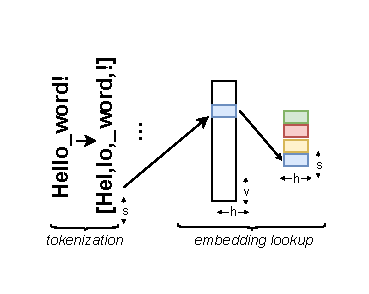
\includegraphics[clip,trim={0 .5cm 0 .5cm}]{images/trigram-classic_encode.pdf}
% 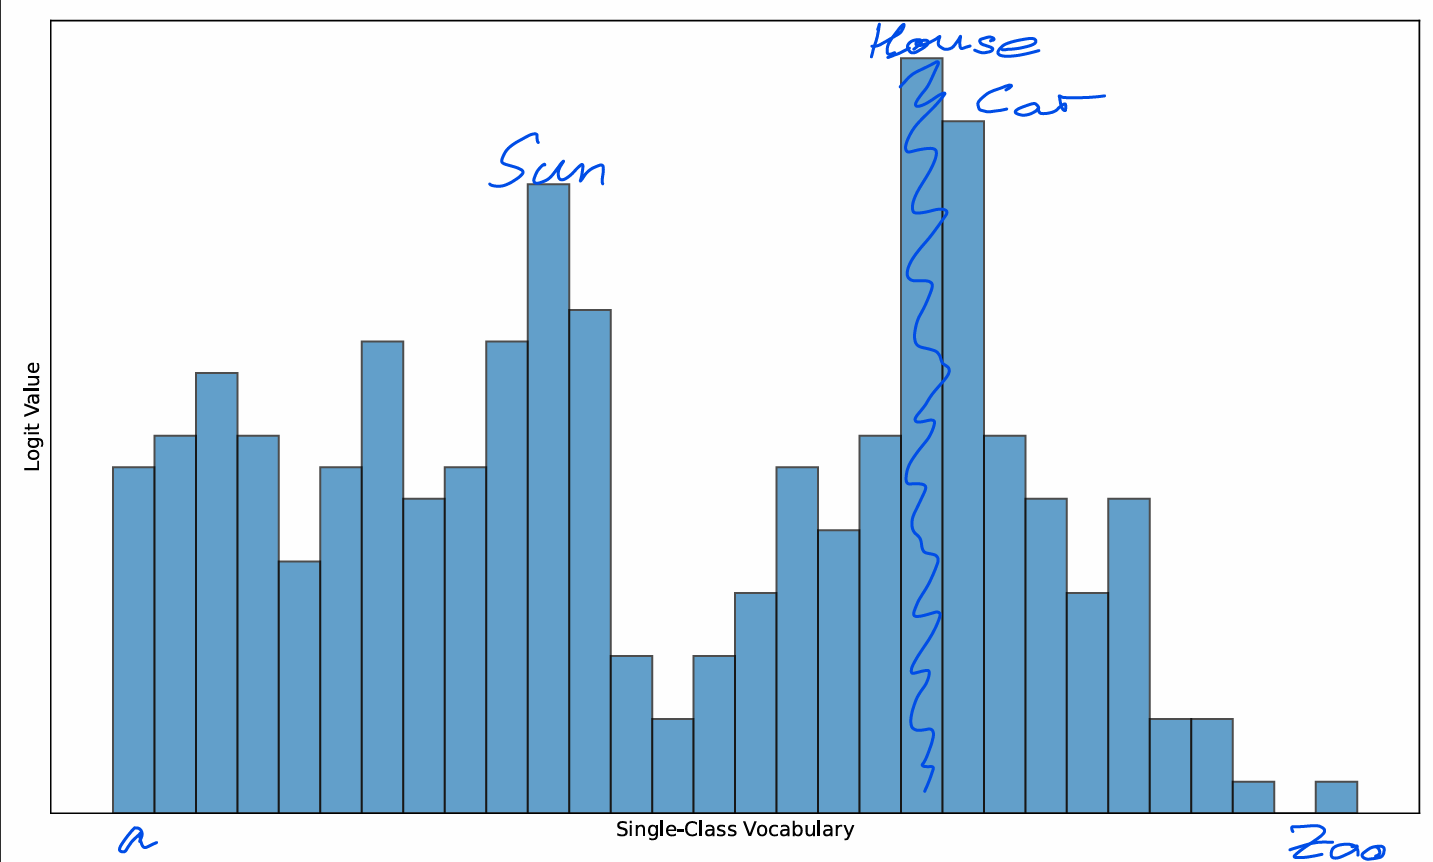
\includegraphics[clip,trim={0 .2cm 0 .5cm},width=.8\linewidth]{images/tokenizer_decode.png}
% \caption{Tokenizer.}
%          \label{fig:tokenization_endecode}
%      \end{subfigure}
%      % \hfill
%      \begin{subfigure}[b]{.45\textwidth}
%          \centering
% 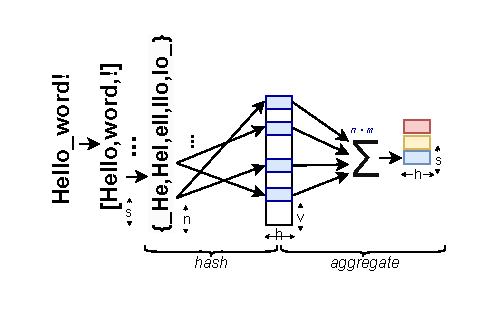
\includegraphics[clip,trim={0 .5cm 0 .5cm},width=\linewidth]{images/trigram-encoding.pdf}
% 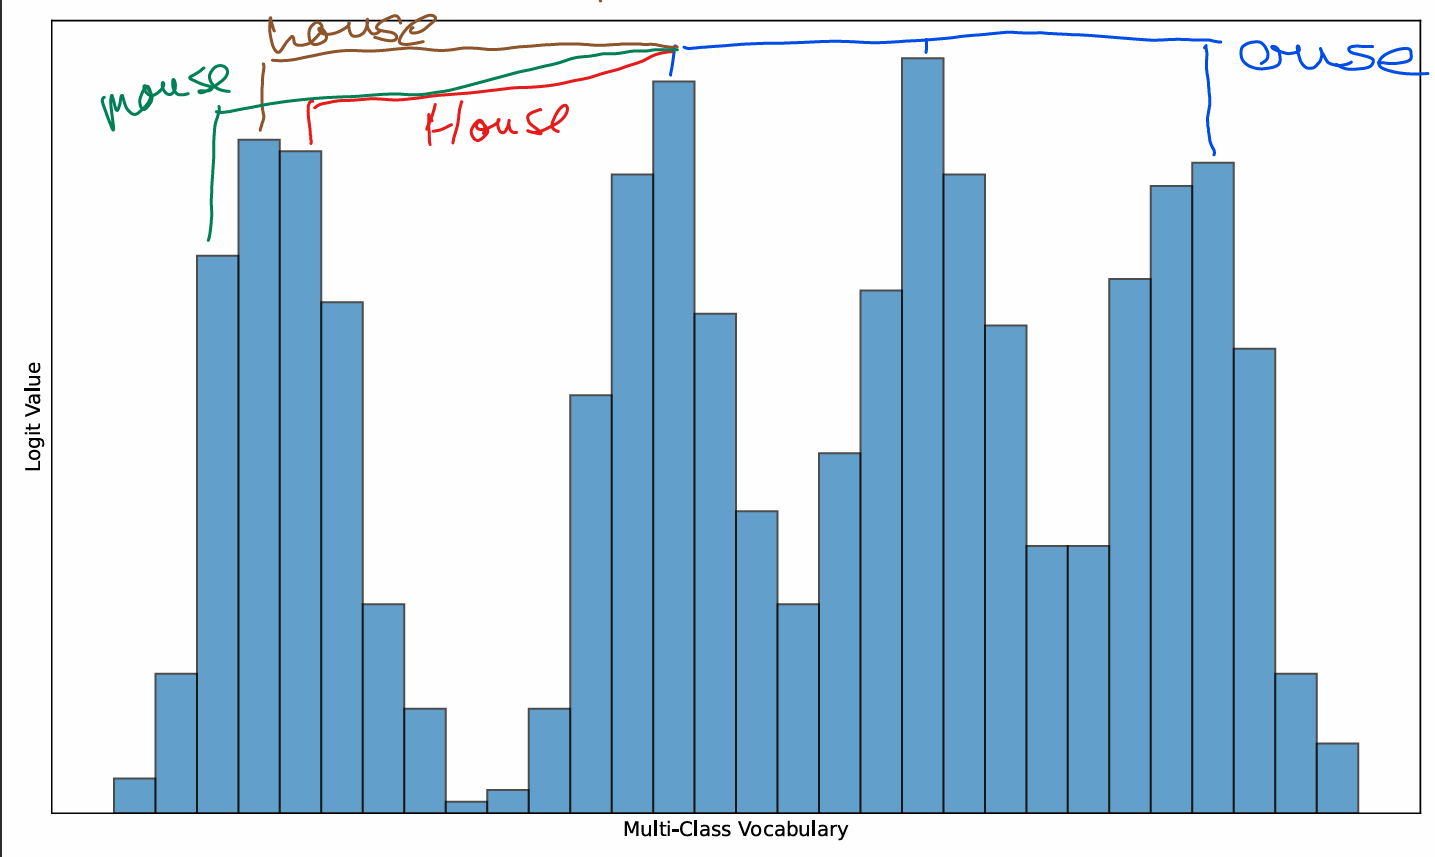
\includegraphics[clip,trim={0 .2cm 0 .5cm},width=.8\linewidth]{images/trigram_decode.png}
%          \caption{\method.}
%          \label{fig:mesa_endecode}
%      \end{subfigure}
%     \caption{Method comparison of Text encoding (top) and decoding (bottom).}
%     \label{fig:endecode}
% \end{figure*}

\begin{figure*}
    \centering
    \begin{subfigure}[b]{.46\textwidth}
         \centering
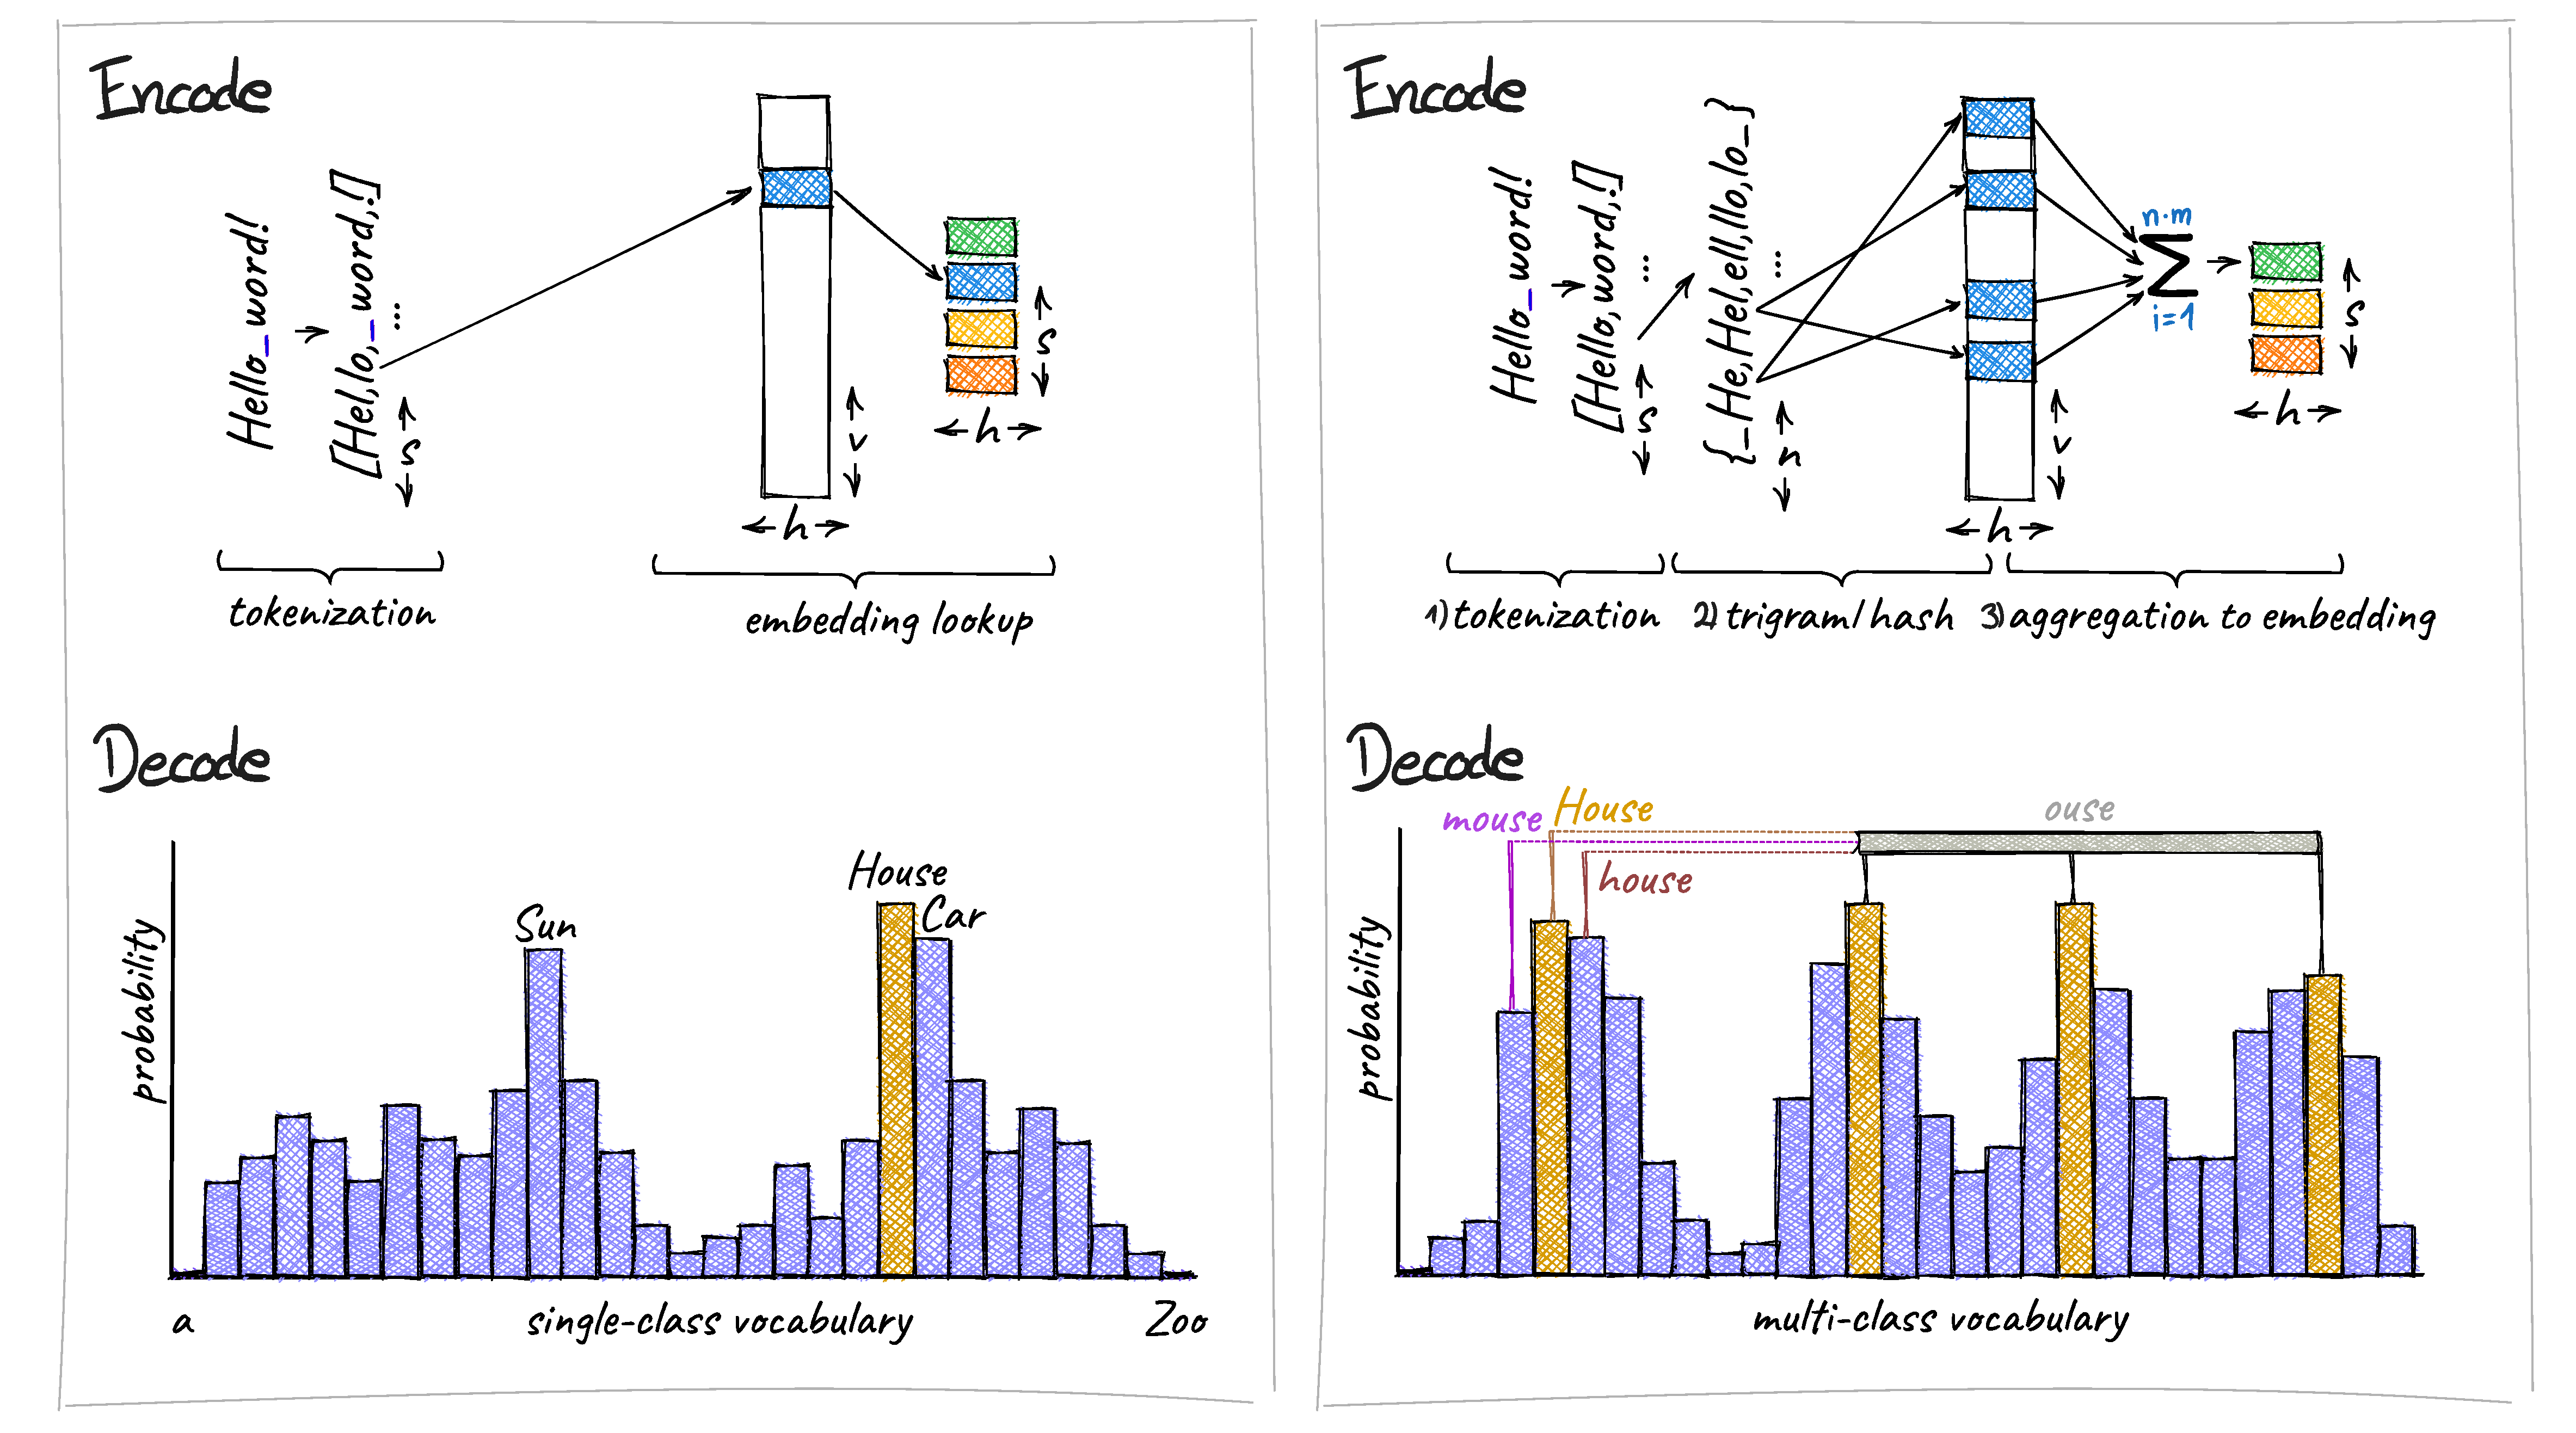
\includegraphics[width=\linewidth,clip,trim={0 0 40cm 0}]{images/figure1_new.pdf}
\caption{Classic Tokenizer.}
         \label{fig:tokenization_endecode}
\end{subfigure}
    \begin{subfigure}[b]{.46\textwidth}
         \centering
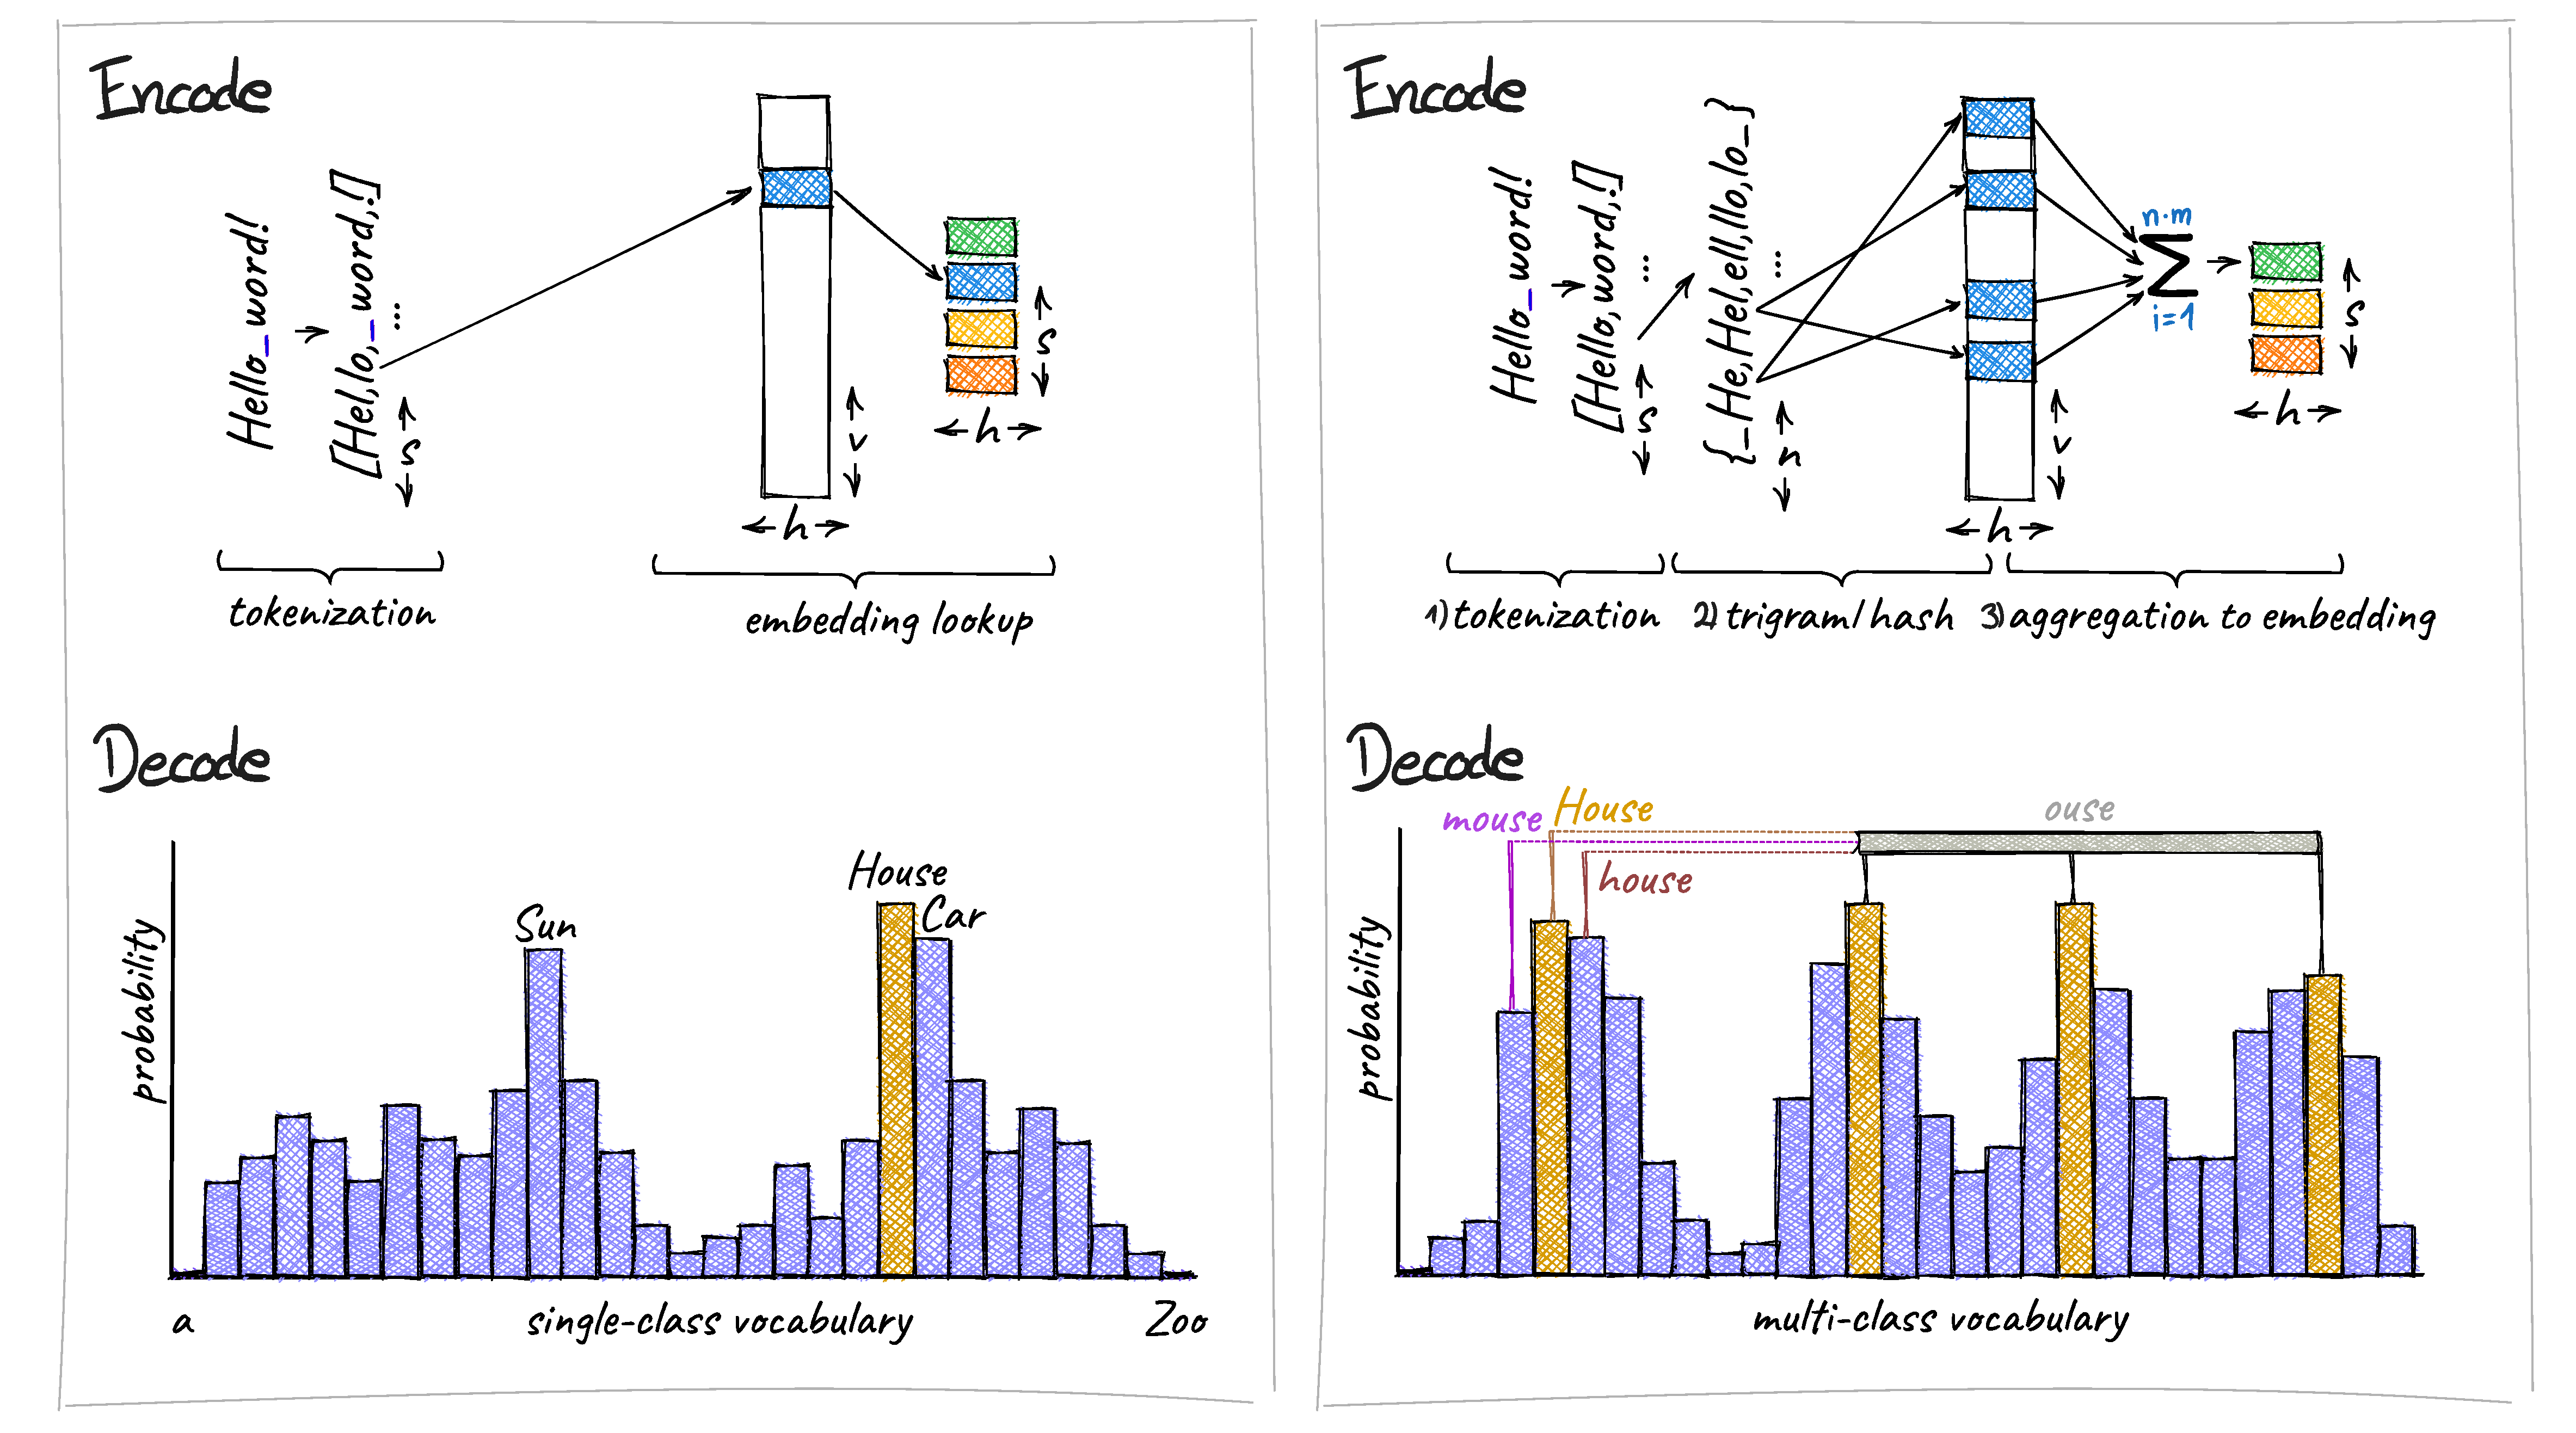
\includegraphics[width=\linewidth,clip,trim={40.5cm 0 0 0}]{images/figure1_new.pdf}
         \caption{\method.}
         \label{fig:mesa_endecode}
\end{subfigure}
    \caption{Method comparison of  classic Tokenization (left) and \method\ (right) for text encoding (top) and decoding (bottom). Classic subword tokenizers learn a single-label vocabulary, i.e. a token is bijectively mapped into a single entry of the vocabulary. Instead, \method\ uses a bijective multi-label mapping over multiple activations of hashed character trigrams. As \method~explicitly models morphological similarities, it enables compression of the embedding layer.}
    %, and  during model training and inference.}
    \label{fig:endecode}
    \vskip -.5em
\end{figure*}


% \section{Introduction}
\section{From Text Representations For Machine Learning}
\label{sec:intro}

%Intro: llm processing, what are tokenizers
% Large language models (LLMs) have recently demonstrated impressive capabilities in the processing of natural language and other types of data.
% The tokenizer is a crucial component of any language-based LLM. It bijectively splits the input text into a defined set of subwords and, together with the LLM's embedding layers, converts the discrete textual data into a numerical representation and back. 
% Consequently, these components heavily shape the training objective and influence what an LLM can process, interpret, and generate. Since their initial conception, the fundamental building blocks of tokenization and embeddings have remained largely unchanged.  
Large language models (LLMs) have shown remarkable abilities in processing natural language and various data types. The tokenizer, an essential part of any language-based LLM, splits input text into subwords and converts textual data into integer representation.
It is built by populating a fixed-size vocabulary based on statistical frequencies in a reference corpus \cite{sennrich2016bpe, kudo2018sentencepiece}.
With the LLM's trained embedding layers, these integers are converted into floating-point representations \cite{mikolov2013distributed, press2017using, vaswani2017attention}. These components significantly shape the training objectives and influence  what an LLM can process, interpret, and generate. Despite advances, the basic principles of tokenization and embeddings have remained largely unchanged in recent years.

{\let\thefootnote\relax\footnotetext{\url{https://github.com/Aleph-Alpha/trigrams}}}

% Subsequently, an embedding matrix is trained to learn a representation for each token in the vocabulary 

Although this approach has served the LLM community well, 
and influential characters target to tokenize all kinds of data to ``lead a new industrial revolution''\footnote{\tiny{\url{https://x.com/tsarnick/status/1801884651986030820?s=12&t=5I__mymj5rXz7lxfplR8Gg}}},
it has significant inherent weaknesses. For one, subword tokenizers require dedicated training and, as such, additional computational resources. Design choices and errors at this stage can negatively impact the downstream model \cite{ali2024tokenizer}. 
Any tokenizer's vocabulary is heavily optimized for the reference corpus, leading to strong drops in performance for, e.g., underrepresented languages. 
We also show that the resulting vocabulary of subword tokenizers is poorly utilized, where up to 34\% of tokens are near duplicates with limited additional information. Despite that, the corresponding embeddings are trained independently. 
These issues have caused a significant expansion in the size of vocabularies and their corresponding embedding layers, with billions of parameters being allocated exclusively for text encoding and decoding.

To remedy these issues and challenge the traditional views, we propose a paradigm shift on how we embed and decode text for LLMs. We present tokenizer-free sparse representations for memory-efficient embeddings (\method) as an alternative to subword tokenizers. We directly embed each word in the input text with sparse activation patterns over hashed character triplets. Consequently, we eliminate the need for subword tokens, thus retaining near-optimal performance across languages. 
Additionally, \method~explicitly models character overlaps between morphologically similar words without the need to learn an embedding for each variant from scratch through a one-to-one bijection. The backbone of the language model will remain free of subword tokenization as we directly encode the textual representation. 
% After all, there is little semantic difference in similar words; 
We argue that the converged embedding of such similar words should remain close and, thus, can be heavily compressed\footnote{The English language contains about $500k$ words, while ``native fluency'' is achieved at $10k$ words \cite{nation2006large}.}.
This exploitation of similarities allows \method~to reduce the size of the embedding layers by $87.5\%$\footnote{Compared to our $64k$ unigram baseline.} and the average encoding length of text by $56\%$\footnote{Compared to Mistral $32k$ avg. of EN, DE, RU, VI, AR.}. In addition to the inherent benefits of \method, the approach remains highly competitive on standard downstream model performance benchmarks. 
Finally, for transfer learning to an unseen language, the \method\ model quickly improves performance, while the tokenizer baseline shows only minor adaptation.


Our contributions can be summarized as follows: 
\begin{itemize} %compactitem
    \item We systematically demonstrate the inherent weaknesses of common tokenization and embedding approaches. 
    \item We propose \method, a powerful and efficient alternative for tokenizer-free LLMs.
    \item We exhaustively evaluate hyperparameters of \method~on established benchmarks by training 1B LLMs from scratch. Our comparison against equally trained models with classic tokenization demonstrates competitive performance despite the significant reduction in compute resources and parameters.
    \item We demonstrate the capabilities of \method~for cross-lingual transfer on continual pre-training %for German 
    on a 3B LLM. % trained from scratch.
\end{itemize}

% \newpage

% %\todo{intro sentence: LLMs, transformer recently blabla}
% Tokenizers form the foundation of modern LLMs. They map from text to numerical representation---and vice versa---and as such enable machine learning on a numerical level at all.
% These projection rules therefore dictate what an LLM can process, interpret, and eventually generate, and moreover its training objective. 
% The most prominent algorithms to train tokenizers are BPE and Unigram, which iterate by either merging or splitting vocabulary entries based on frequency estimates over a reference corpus. They are given an initial set and converge when a desired vocabulary size is reached. 
% \todo{small visual needed?}


% %llm processing stages - i.p. decoding/ objective
% Given a fixed Tokenizer, Fig.~\ref{fig:pipeline} shows the stages of an LLM  text generation process.
% In the beginning (I), the input text is encoded by the tokenization rules into a sequence of integers. These integers are looked up in an embedding layer. It is the learned representation mapping of the tokenizers' vocabulary into the numerical hidden dimensions of the actual model. As such, it is of dimension $embed = \# vocab \times hidden$. This process is shown in more detail in Fig.~\ref{fig:classic_encode}.
% After processing the sequence through the transformer model, it is again mapped through the ``LLM head'' into a sequence of vocabulary likelihood values, and as such requires another matrix of $embed$ size.

% The training objective is usually to predict the next token and as such is formulated as single-class prediction with a cross-entropy loss. 
% The output of the model will therefore be of dimension of the vocabulary size.  As such, the output values can be transformed and interpreted as the ``likelihood'' to the next token. ``Greedy decoding'' may be performed by taking the argmax ---the predicted class--- to derive the next token. Given an input text, the model iteratively predicts chunks of words that can be appended to the input or mapped back into text, until a desired length is reached. Note that, as such, the number of tokens required to resemble a word directly influences the required inference costs.
% \todo{ single class prediction can be error-prone}

% \begin{figure}
% \centering
% \begin{subfigure}{0.7\linewidth}
% 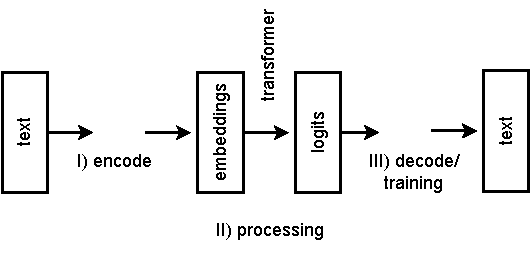
\includegraphics[width=\linewidth]{images/trigram-pipeline.pdf}
% \caption{pipeline stages of NLP transformer architecture I) conversion of text to embeddings II) processing III) decoding of logits to text. we investigate I and III. 
% \todo{put input dimensions!}}
% \label{fig:pipeline}
% \end{subfigure}
% \begin{subfigure}{0.7\linewidth}
% 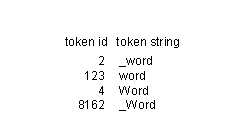
\includegraphics[width=\linewidth]{images/trigram-tokenizer_example.pdf}
% \caption{examples of duplicates in tokenizer todo show splits of woRds etc \todo{see appendix}}
% \label{fig:duplicates}
% \end{subfigure}
% \caption{pipeline and tokenizer impact}
% \label{fig:pipe_token}
% \end{figure}


% %flaws of statistical tokenizers algorithm in general
% Due to the purely statistical training objective of tokenizers, its vocabulary includes many suboptimal chunks that may split a word on a linguistically wrong ---but frequent--- position. Moreover in SOTA LLM tokenizer vocabularies up to $35\%$ duplicates can be found,  that differ only in a leading white space or capitalization as shown in Fig.~\ref{fig:duplicates}\todo{- Fig.~2a}\todo{ref table}
% \todo{referencs}. 
% Each of these tokens represents linguistically almost the same information but its numerical representation is entirely independent initialized and trained from scratch. 
% Earlier versions even included a significant amount of frequent occurring numbers, which was recently decided by the community to be most accurately predicted when the vocabulary only includes single digits. However, it remains unknown what the best representation is.\todo{refs}

% %flaws of resulting llms given a tokenizer
% Note that a tokenizer is trained and fixed before the actual LLM  training.
% As such, an LLM implicitly is optimized to interpret and generate character splits reflected by the tokenizer ---and the data distribution with which the tokenizer was trained.
% %Performance rating of a transformer is difficult, usually fertility is used. 
% Naturally, the use of languages ---or more general document formattings--- that were already presented in the tokenizer training will result in less tokens per word on average. In particular, it will result in a more precise entropy split, as less concepts are shared amongst a single token and as such need to be interpreted by its context. Arguably, this already restricts the later use case or fine-tuning capabilities of a pre-trained LLM \todo{reference}.
% The trained model performs best and most efficient on data the tokenizer was trained with as well. Later extension of the tokenizer, even for downstream model fine-tuning, is nontrivial. 
% This is in particular critical as pretrained models cost billions of dollars\todo{ref}.
% Consequently, recent models are being released with a vocabulary that exceeds $250k$ tokens to compensate for the risk of later degenerate downstream performance. 
% \todo{mention short encoding sequences are needed as maximal sequ length size is limited/ active research}
% \todo{tokenizer training, and large-text encoding is computationally very intense -> corpus needs to be reduced -> nonoptimal vocab}

% %flaws of tokenizer size for model training
% Notably, the embedding layer and the language model head  are the largest matrices of an LLM, of dimension $\#vocab \times hidden size$. 
% %For gemma it thus is $2\times 250k \times 4k$ weights.  
% For LLama3-7B this results in $2\times 128k \times 4k$ floats ---2GB RAM allocation for 2bytes per float precision--- or 15$\%$ of the total model weights. The actual memory consumption during training requires another factor $2$ for the backward gradients and $1.75$ for the loss computation and optimizer step.
% As such a significant amount of the available 80GB RAM available on modern GPUs used to train these models are solely allocated for this embedding and computationally underutilized. \todo{in practice often iterated loss computed with specific cuda kernels to reduce memory}
%  This issue becomes even more severe for the recent trend of smaller (e.g. 1B) on-the-edge models that are supposed to execute well on few specific tasks and restricted hardware resources. As such, smaller models require a nonoptimal smaller vocabulary, which overcomplicates the input or renders inference inefficient, even though the model is presumed to be less performant by number of parameters already. 

% %this work
% In this work, we present for the first time an alternative to tokenizers to embed and decode text. In particular, we do not rely on an embedding matrix of dimension $250k$, but show that a reduced size of $4k$ entries suffices to encode language, without sacrificing performance. This already renders the memory footprint and training objective and, as such, particularly paves the way towards performant small models.
% We, moreover, do not produce word splits based on a fixed vocabulary. Each word gets encoded into exactly one embedding based on a sparse activation pattern of our embedding function.
% This reduces \todo{fertility} to exactly $1$. Moreover, it simplifies the computationally intense tokenization process, as no complicated rule set is to be met.
% Finally, we switch from single- to multi-target classification, which is arguably a more robust training objective.
% As we will show, our approach is generic applicable amongst languages and code documents, and leaves room for constitutive research. 
% Moreover, we can explicitly model the overlap between spelling variations of words, and, as such, various capitalizations are not independently learned from scratch or randomly split into parts.

% To demonstrate the effectiveness of our approach, we train a series of 1B models from scratch for \todo{XXX} tokens on the english slimpajama dataset. Comparing our approach with $4k$ embedding size and a specific unigram tokenizer trained on slimpajama with vocab size $64k$, we improve the language model capabilities by $\todo{XXX}\%$ on standard language model benchmarks. The memory footprint is reduced by $\todo{XXX}\%$ and the word fertility by $\todo{XXX}\%$.
% Finally, to estimate model-transfer capabilities, we continue training on a dataset in the german language. Our approach improves $\todo{XXX}\%$ in german language benchmarks and $\todo{XXX}\%$ on fertility in german.

% \begin{figure}
% \centering
% \begin{subfigure}{0.7\linewidth}
% 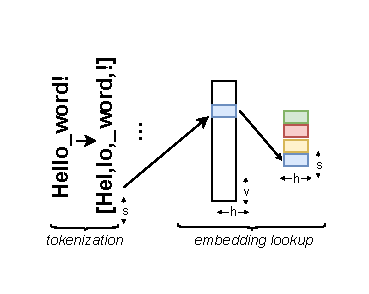
\includegraphics[width=\linewidth]{images/trigram-classic_encode.pdf}
% \caption{encode}
% \label{fig:classic_encode}
% \end{subfigure}
% \begin{subfigure}{0.7\linewidth}
% 
\includegraphics[width=\linewidth,clip,trim={0 23.5cm 8cm 0}]{images/trigram-classic_decode.pdf}
% \caption{``greedy'' decode (argmax)/ training objective  (one-hot single-class)}
% \label{fig:classic_decode}
% \end{subfigure}
% \caption{classic tokenization,  s sequ length, k hidden size l vocab size. $s\cdot k$, $s=4,l=64k$}
% \end{figure}

% \begin{figure*}
% \centering
% 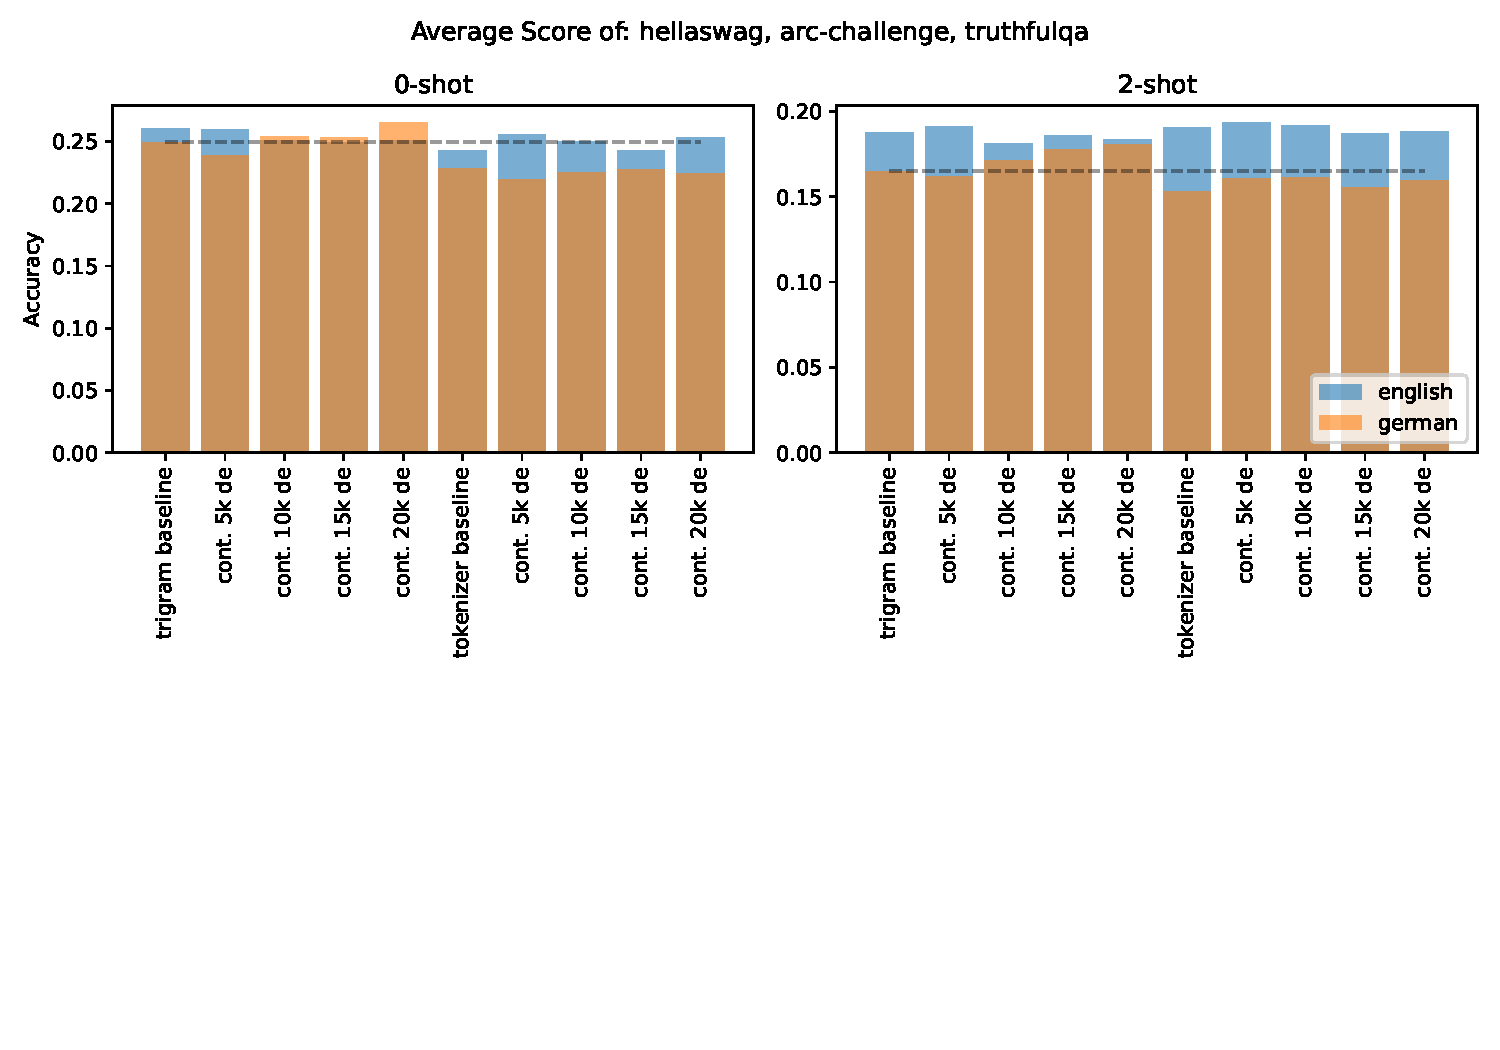
\includegraphics[width=.8\linewidth,clip,trim={0 6.5cm 0 0}]{images/plot_de_en_avg.pdf}
% \label{fig:classic_decode}
% \caption{Continued Fine tuning on german language using occiglot Todo: Line plot \todo{eng separated}}
% \end{figure*}




% \begin{figure}
% \centering
% \begin{subfigure}{\linewidth}
% 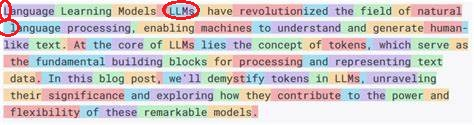
\includegraphics[width=\linewidth]{images/draft/tokenization.jpg}
% \caption{before: }
% \label{fig:encode}
% \end{subfigure}
% \begin{subfigure}{\linewidth}
% 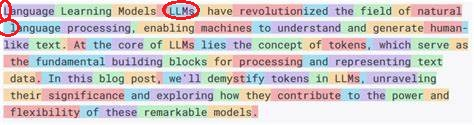
\includegraphics[width=\linewidth]{images/draft/tokenization.jpg}
% \caption{\todo{after: all cool.} }
% \label{fig:encode}
% \end{subfigure}
% \caption{tokenization example. many words (e.g. ``language'') need to be present with whitespace and without, with capitalization and without. LLMs is chunked into 2 parts, needs to be assembled by attention.}
% \end{figure}


\section{Classic Tokenization Principles}
%\section{Background}
\label{sec:background}
Before we derive \method~in detail, let us first establish some basics of how LLMs traditionally encode and decode text. Most LLM operations
%, in particular during training, 
are performed in floating-point numbers through a series of matrix multiplications and non-linear activation functions.
Consequently, we require techniques that map discrete textual inputs into floating-point representations and inversely transform the predictions of the model back to text. 
%It transforms vectors representing input text into output vectors containing preferences to text predictions. As such, the basis for the processing and interpretation capabilities of a large language model is the mapping of textual to numerical data, the objective training function, and the reverse mapping of predictions to output text. 

% \subsection{intro}
Traditionally, the first step in this process is to split any textual input into small chunks referred to as \textit{tokens}. Generally, these tokens can take arbitrary formats, spanning numerous characters, a single or even multiple words, and may also contain special characters. The latter can be particularly useful to encode programming languages. 
A \textit{tokenizer} comprises the steps and rules that are necessary to dissect a text into a sequence of tokens. Importantly, the total number of tokens is restricted, and we refer to the set of \mbox{all unique tokens as the \textit{vocabulary}.} 
%such that each one can be assigned 
%Clasically, a tokenizer is trained on a large corpus of representive and cleaned data to solve this task. It splits the input text into text-chunks, so called ``tokens''. 
%Apriory there are no restrictions to the format of a token. It can span multiple characters ---or even words--- and contain various special characters. The latter is particularly useful, for instance, with code programming languages, to integrate commands into a single token. 
%where combinations like ``$/*$'' form a command, for a block-comment in the Java programming language,  can be integrated into a single token.
%The tokens form the ``dictionary'' and are each assigned a unique number.

Each token in the vocabulary is assigned an integer \textit{token-id}, wherefore tokenizers produce a sequence of token-ids for any textual input. 
Next, a large matrix of dimensions \emph{vocab size $\times$ hidden size}, an LLM's \textit{embedding layer}, maps each token-id to an internal representation as a floating point vector (cf. Fig.~\ref{fig:tokenization_endecode}). 
%
%Given a fixed tokenizer, the actual language model can be trained. The textual training data is first transformed into the vector of its token-ids. The first layer of the LLM is known as the ``Embedding Layer''. It is a  matrix that maps token-ids into a vector of floating point numbers as shown in Fig.~\ref{fig:classic_encode}.
%, e.g. by multiplying one-hot vector of id to the matrix. A diagram of this encoding scheme is .
To produce new text, generative models are trained auto-regressively. That is, they iteratively predict the next token, which is appended to the input text. 
Therefore, the training objective is formulated as a classification problem: a one-label prediction of the next token over the entire vocabulary. 
%due to the bijective mapping of tokens to integers. 
Consequently, the last layer of the model---the \textit{LM head}---is a projection into the size of the vocabulary and thus also of dimension \emph{vocab size $\times$ hidden size}. For decoding, we can, for example, always select the token with the highest assigned value, which is called \textit{greedy sampling}.
%By appending this token-id to the input, we iteratively generate a sequence of continuations.
The output text is produced by looking up the corresponding text snippet of each predicted token-id in the vocabulary.
%As such, the last layer, called ``LM head'', is a projection into the vocab-size dimension. The loss function is cross-entropy between the last vector and the next token-id.
%To decode the actual predicted text, during inference, usually the maximum index of the last vector is used as a reference to the next token-id. This id can be looked up in the dictionary and be replaced by its actual substring. This procedure is called ``greedy decoding''.

Generally, it is desirable to encode any text in as few tokens as possible to reduce computational cost. 
At the same time, different semantic concepts should be separated into distinct tokens to ensure good language comprehension. The combination of both objectives is usually best satisfied by encoding each word as one token. 
%\todo{However, since all matrices are randomly initialized, each writing variation, in particular letter capitalizations, needs to be learned anew and as such be represented in the training data.
% Furthermore, this leads to very large vocabularies and embedding layers, which becomes a computational burden, as they already extend to multiple billion parameters.}


%Generally, we prefer as a text encoding smaller sequences of tokens, as each token adds computational cost, an additional dimension to the processed matrices.
%Moreover, it is desired to properly separate semantic concepts into distinct tokens, as too ambiguous gradients on tokens may lead to degenerate predictive performance. 
%However, both objectives require a larger vocabulary, which in turn allocates more GPU memory and increases language model training as well as text tokenization costs. 

% \paragraph{Performance Metrics.}
% \paragraph{Evaluation Criteria.}
%\paragraph{Comparison Metrics.}
% Measuring the performance of tokenizers is not straightforward. 
% Its primary objective is to generate the best possible language model after training, which is costly to ablate \cite{fraunhofer paper}.
% Afterall, it is yet unclear what the best input to a NLP model is.
% Arguably, in particular in a one-class prediction setting, we want to separate semantic entropy as strict as possible into separate classes. However, quantifying this is complex, as it requires a language model on its own. 

% The most prominent statistical values to compare tokenizers are ``fertility'' and ``Normalized Sequence Length'' (NSL).
% The fertility score refers to the average number of tokens generated per word in a text. As such, 1 is the minimal value, whereas it is not defined what a word is - e.g. for concatinated words by hyphens.
% NSL compares the average number of tokens generated on a corpus with a baseline tokenizer. This is in particular useful, as words are even less defined programming language.

% Note that both metrics favor tokenizers that produce less tokens. While this speeds up required training and inference iterations, it completely neglects I) the actual meaning of tokens, II) the required model parameters, and III) the computational costs of the tokenization process itself. 

% In our evaluations, we therefore also include I) overlap percentage of tokens in a vocabulary, disregarding whitespaces and capitalizations,  II) percantage of embedding layer compared to the ``actual'' model parameters, and III) runtime estimates of the huggingface implementations.
% Finally, we also probe the generalizability of the tokenizer by performing succinct fine-tunings of pretrained models on a second language, without altering the tokenizer.   \todo{move last paragraph to experimental setup ?}




\subsection{Tokenizer Algorithms}

The vast majority of LLMs utilize a tokenizer built with one of two approaches. Both progressively build up tokenization rules and their vocabulary based on statistics in a reference corpus.

\textbf{Byte Pair Encoding (BPE).}
%BPE~\cite{sennrich2016bpe} was originally designed for data compression and later adapted to NLP tasks.
BPE \cite{sennrich2016bpe} starts with a set of all characters as individual tokens. Progressively, the most frequent token pairs occurring together in the training documents are merged.
The resulting new token and the merging rule are added, and the training is completed \mbox{when the desired number of tokens is reached.}

In order to encode text with the trained tokenizer, BPE splits the input into individual characters and applies the lowest-ranking merge rule until no more are applicable. This exhaustive search can become computationally intensive, especially for long input sequences and large vocabularies. 
%Due to the exhaustive search, this can become compute intense, i.p. for very long input sequences and vocabularies.
%%Text-detokenization maps directly into the vocabulary list. 
%\todo{add formulars / required?}
%\todo{reference models}


\textbf{Unigram.}
%\mb{I don't think we need to get this technical. a high level understanding should be enough}
%
Unigram~\cite{kudo2018sentencepiece} operates inversely to BPE. 
First, it splits the training corpus into a large set of reference words and their respective frequencies. The vocabulary is initially populated with all possible substrings of these words.
%reference set of words $C$ with frequencies and all possible subsets of words as vocabulary $V$.
At each iteration, Unigram computes a loss of the current vocabulary with respect to the training corpus for all possible tokenizations. The least influential tokens are then removed until the desired vocabulary size is reached. 
%
% Its training objective is to find a reduced $V'$ of maximal size that maximizes the log-likelihood $L(V')=\Sigma_{w\in C} \log (\todo{\Sigma}_{x\in S(w)\subseteq V'} p(x))$ on the data corpus using the Expectation-Maximization algorithm. Here $S(w) \subseteq V$ denotes the set of all possible tokenizations of the word $w$, and $p(x)$ is a frequency approximation on the training corpus $C$. As such, the vocabulary gets ranked by its loss influence and iteratively least influential tokens are removed until the desired vocabulary size is reached.
For text encoding, the Viterbi algorithm is applied to determine the most preferred segmentation of a given word based on the ranked available tokens.

The text decoding in both cases maps directly back into the vocabulary list and the respective sub-words. 
To ensure that every word can be represented, a ``byte-fallback'' into unicode is often used for characters not present in the vocabulary.
% Unigram more than BPE during encoding due to the need to compute probabilities for each potential tokenization.





%\subsection{Discussion \ps{better title? What about: Limitations or Shortcomings\\ ChatGPT says: Facing the Flaws}}
\subsection{Facing the Flaws} \label{sec:flaws}
% However, unlike BPE, its tokenizer does not guarantee a deterministic tokenization, as it uses a probabilistic model to select the best tokenization. This can lead to different tokenizations for the same text in different contexts. \todo{is this actually correct?}

% Tokenizers can handle out-of-vocabulary words by breaking them down into known subwords.
% Frequent occuring words as such are represented as a single token which lowers average fertility. 
% Similarly for compositional subwords, most frequent endings can be found as well. As a last base, byte-fallback is used to ensure that each word can properly be encoded ---in the worst-case into its byte representation.



% \textbf{Shortcomings BPE vs Unigram.}
Common to both methods is a set of distinct flaws.

%

\textbf{Large Vocabularies F1)} Words that do not appear in the vocabulary are split into multiple tokens and, as such, require more compute during model inference and training.
To avoid out-of-vocabulary words and to achieve the best downstream representations on a diverse set of languages and tasks,
%, which assumably perform worse than fully represented words, 
researchers tend to use ever larger vocabularies. Although some models still rely on a $32k$ vocabulary \cite{touvron2023llama2, jiang2023mistral}, more recent releases go up to $128k$ \cite{meta2024llama3} or even beyond $250k$ \cite{mesnard2024gemma, cohere2024commandr}. 
Large vocabularies, in turn, require large embedding and head layers. 
%\todo{say that transformation is basically duplicated in parameters}
For example, Command-R \cite{cohere2024commandr} with a hidden dimension of $12,288$ and a vocabulary of $256,000$ tokens uses $6.3B$ parameters only for the embedding and head layer.
Naturally, a large number of parameters complicate model training and may require 
%In particular, such dimensions require 
advanced sharding techniques such as ``model parallelism''.
%to efficiently fit computations for the backward gradients and optimizer steps.
Even the tokenization itself can become \mbox{(CPU-)} computationally intense for large documents and vocabularies.
Naturally, embedding matrices of this scale are generally not an option for smaller ``on-the-edge'' models. 
%Consequently, the hidden dimension will be reduced significantly.
Nevertheless, they still occupy a large portion of parameters in smaller models, e.g. 40\% for Gemma-2B \cite{mesnard2024gemma}. 


\textbf{Duplicate Tokens F2)} Furthermore, the allocated vocabulary is expected to be poorly utilized due to the statistically likely occurrence of near-duplicate tokens. 
Most prominently, a significant portion of tokens appears multiple times, only differing in capitalization or the existence of a leading whitespace (\emph{cf.} Sec~\ref{sec:exp_flaws}).
For example, to spell all 64 substrings and variations of the word ``\_words''\footnote{$\_$ represents a whitespace.}, we require a total of 37 unique tokens (\emph{cf.} App.~Tab.~\ref{tab:word_prefixes}). 
Since the corresponding embeddings of all tokens are independent and randomly initialized, the representation of each duplicate token needs to be learned from scratch without exploiting morphological synergies.
%As each token is independently initialized, the meaning of each duplicate needs to be learned independently as well, from scratch.
Further, large embedding layers are purely utilized since some tokens will rarely occur. The corresponding embedding weights of these tokens are thus seldom active while still requiring compute.
%\mb{State that this also means that activation in the embedding layer are badly distributed with a long tail}


\textbf{Training data overfitting F3)} As discussed above, these tokenizers require dedicated training before the actual model training. In addition to the added computational overhead, the data selection and potential mistakes during tokenizer training have significant impact on the subsequent LLM \cite{ali2024tokenizer}. 
%The data selection for the training of the tokenizer ---and as such the outcome of the actual tokenizer training--- highly inflict the best-case outcome of the actual model training, and in fact bias the performance on later downstream applications.
For natural language, for example, this paradigm may result in a vocabulary tailored to one language (usually English) and consequently drops in performance for others, especially those not explicitly included. 
The resulting LLM may still be somewhat adapted to other languages since many similar low-level structures \cite{nikolov2013exploiting}. However, its overall training and inference performance will not be as efficient as we demonstrate.

%In the same vein, tokenizers are narrowly optimized for the targeted domain. 

In contrast, \method~addresses all of these disadvantages. It is computationally efficient and performs good tokenization across languages without duplicates. It drastically reduces the parameters required for text encoding, exploiting word spelling similarities. Importantly, none of these improvements sacrifices downstream model performance.



%can be computationally intense 

%OOV

%$>> 64k$ (i.p. embedding is $64k \cdot hidden$). doesnt work 

%\mb{repeated tokens (capitalization, whitespaces), i.e. bad utilization of vocab}

%\mb{Highly specific for one domain/language. Significant loss in performance/efficiency for non-english (usually) or requires huge vocab}

%\mb{Large vocabs lead to large embedding layers. Can make up a signficant portion of smaller LLMs and results in bad scaling}



\section{\method}
\label{sec:trigram}
A key motivation for \method~is the intuition that minor differences in spelling, like leading whitespaces or capitalization, do not hold enough entropy to justify entirely independent tokens. 
%
\method~directly encodes morphological similarities by representing each word as a multi-label encoding of its character triplets. This designed overlap between words allows us to significantly reduce the size of embedding layers.

We now derive \method's approach to text encoding and decoding and discuss implications on LLMs in general. We provide a visualization of each step in Fig.~\ref{fig:mesa_endecode} and pseudo-code in App.~\ref{app:mesa_algo}.
%based on spelling similarities, we show that a space of $8k$ embedding entries is sufficient without sacrificing downstream performance (for two languages).

%
%Arguably, minor differences in spelling---like leading whitespaces or letter capitalization---do not hold enough entropy to justify an entirely independent token training.
%\todo{refs} \todo{move to intro?}
%As such, one can assume that a lot of compression can be done to avoid tokenizer vocabularies exceeding $100k$ entries in an optimal scenario. 
% \ps{add one Algo for 3.1 and 3.3}

% \mb{mention the core idea in the beginning (trigram embeddings)} \bd{intro is enough as it is}

% \mb{mention "one hot encoding"} \bd{in 3.2 but not before}

\subsection{Text Encoding}
\label{sec:encoding}
\textbf{Step 1: Word splitting.} First, we rigorously split the text by digits and non-alphanumeric characters. The resulting splits, therefore, contain entire words, digits, or special characters.
We consider each digit separately, as it is standard in SOTA LLMs (\emph{cf.} Tab.~\ref{tab:language_fertility}). Specifically, we include the 10 digits $0$ to $9$, and otherwise, we rely on attention to comprehend larger numbers or mixtures with characters.

By definition, we represent each word with a prefixed and suffixed whitespace. In particular, we assume that an entire word is encoded into a single embedding, and analogously, we predict an entire word at once.
Consequently, we no longer need to explicitly model whitespace as a character and eliminate near-duplicate tokens. 
Nonetheless, we add a dedicated ``whitespace'' and ``non-whitespace'' token to the tokenizer. These special tokens allow us to model cases where substrings should (not) be concatenated with whitespace, e.g., single digits of larger numbers. 
%
To reduce their need, we further add a rule-set that favors \mbox{(non-)}whitespace in front or after certain characters. Generally, we prefer to add no whitespace after a digit embedding and similarly no whitespace before punctuation.  
A detailed description of the rule set is found in App.~\ref{sec:whitespace}.

Considering the example in  Fig.~\ref{fig:mesa_endecode}, the input text ``Hello\_word!'' would be tokenized as [`Hello',`word',`!'].

\textbf{Step 2: Encoding.} Next, we define a robust hash function that uniformly encodes a token into $n$ descriptors, where $n$ usually equals the word-length\footnote{Only exceptions are unicode fallbacks.}.
Specifically, we apply convolutions of size three and byte-wise stride to each word. This operation yields a set of character triplets, which we refer to as ``trigrams''. 
Consequently, ``Hello'' is decomposed into \{\_He,Hel,ell,llo,lo\_\}.
Trigrams usually contain enough information about the relationship between letters to reassemble the word from the unordered set. 

Subsequently, we project each trigram descriptor into a sparse hidden representation vector of $m$ ``active entries'' on the embedding layer. 
Specifically, \method~calculates $m$ numerical hashes of each trigram, which can be considered as identifiers.
We map these into the LLMs embedding matrix by calculating each hash value \texttt{modulo} $v$ to identify the active indices. The selection of vocab size $v$ is further explained in Step 3.

Overall, we obtain $n\cdot m$ total activations for any single word.
To further exploit word similarities and bootstrap training, we calculate $k\in [0,m)$ out of these hash calculations with the lowercased trigram.
%
This mapping from trigram to hidden representation is static and can be precomputed\footnote{Note that there are only $256^3\approx 16.7M$ trigrams.}.
%superpositions. The actual occuring subset is much smaller,
%e.g., the vocabulary of the LLama3-Tokenizer only covers $12k$ superpositions;
%}.
%To further exploit word similarities and bootstrap training, we further let $k < m$ activations of a trigram overlap with its lowercase counterpart.


\textbf{Step 3: Aggregation.}
Similar to classic embedding approaches (\emph{cf.} Fig.~\ref{fig:tokenization_endecode}) \method~also utilizes an embedding matrix of dimension $v$ with hidden size $h$. However, we do not have a fixed vocabulary, whose size dictates $v$. Instead, we can independently choose $v$ as a hyperparamter with words and trigrams sharing individual entries to better encode similarities. 
%We map each trigram into $m$ activations in the embedding matrix by calculating each hash value \texttt{modulo} $v$ to identify the active indices. \bd{das ist step 2, da stehts auch schon more detail -> see appendix}
%Specially, we project each trigram into the embedding matrix $m$ times by calculating \texttt{modulo} $v$ for each of the $m$ integer hash values. 
Lastly, we sum all $n\cdot m$ embedding entries to produce the final one embedding corresponding to a word, such as ``Hello''.
%\ps{Aggregates the sum? how?}Step 3 aggregates the sum of all  activated $n\cdot m$  embeddings to form the final single embedding, which represents the textual word.

Note again, that we utilize a significantly smaller number of embeddings than there are trigrams. While their hashes may naturally overlap, we ensure the uniqueness of the  entire patterns through the $m$ simultaneous hashes. As we ensure that trigram encodings do not collide, neither will the word encodings.

\subsection{Training Objective \& Text Decoding}

As \method's representation of a word is now a multitude of activations, we reflect this change in the LM head, as well (\emph{cf.} \textit{Decode} sections in Fig.~\ref{fig:endecode}, App. Alg.~\ref{alg:encode},\ref{alg:decode}).
%Notably, our representation of a word is a multitude of activations, and not a one-hot single-class encoding as in classical tokenization approaches. 
%Naturally, we reflect this encoding in the LLM head, that is, when predicting the next word.
In particular, we change the target loss function from classic single-label binary cross-entropy (BCE) to a multi-label (ML) BCE over all $n\cdot m$ activations of the next word targets: 
\begin{equation*}
\small\mathcal{L}^{ML}_{BCE} \small\textstyle = - \sum_{j=1}^{v} [y_{j} \log(\hat{y}_{j}) + (1-y_j)\log(1-\hat{y}_{j})],
\end{equation*}
for $\hat{y}$ being the LM's prediction and  $y$ the binary  target vocab labels with $\sum_{j=1}^{v} y_j  =  n\cdot m$.
%$\sum_{j=1}^{v} \mathbb{I}(y_j = 1) =  n\cdot m$.

%\ps{Why is this not a dedicated section anymore?}
%\bd{they belong together just as we do <3}
Next token decoding is shown in Fig.~\ref{fig:decode}. We first assemble a dictionary of all possible next words and pre-compute their activation patterns.  
%For the next word prediction, we do not obtain a probability distribution, on which we can just apply the argmax and lookup the token position in the dictionary.
%Instead, we first assemble a dictionary of possible next words, and for each word compute its activation pattern. 
Importantly, only $n\cdot m$ out of $v$ entries will be non-zero for each word, and since we choose $m <\!< v$, the dictionary matrix can be encoded as a sparse matrix, thus improving runtime.
In addition, note the pattern similarity between similar words, as previously described.
The last hidden layers' output $h$ is sigmoided, and multiplied with the dictionary matrix.
Finally, we compute the average sigmoid value per dictionary entry, $h'$, to sample the next word, e.g. using standard argmax. Overall, for a dictionary with $512k$ entries, this procedure only marginally increases the decoding runtime due to the sparse property of the activation patterns. Further description, along with pseudocode, detailed depictions, and step-wise runtime analysis can be found in App.~\ref{alg:decode}. 

Note that the decode matrix is not required during training, and can dynamically be exchanged. We generate it by sampling the top-$500k$ occurring words in the training dataset, and dynamically adding the missing words of the prompt. 
%We multiply this dictionary matrix with the predicted logits values of the LLM to finally obtain the argmax prediction of the next token.
%Importantly, the sparsity of the matrix makes this multiplication computationally efficient. 
% Further, the mapping is not part of the learnable model paramters and does not need to be trained.
% \todo{elaborate decode further}

\subsection{Distinctions of paradigm shift}
% \ps{merge this into the previous subsection?}
Notably, this paradigm shift to a multi-class vocabulary allows for more semantically robust decoding. With the classical approach, the distinctly noisy learning process can lead to unrelated concepts appearing among the top predictions (\emph{cf.} `\textit{House}' and `\textit{Car}' in Fig.~\ref{fig:tokenization_endecode}). This effect can have a significant impact on next token sampling and potentially devastative outcomes for model modifications such as compression~\cite{deiseroth2024divergent}. 
In contrast, the trigrammification and resulting embedding overlap of similar words with \method~
%in combination with multi-label predictions 
inherently favors similar words during decoding  (\emph{cf.} `\textit{ouse}' in Fig.~\ref{fig:mesa_endecode}).
Moreover, activations in the embedding and LM head are more uniformly distributed, leading to better parameter utilization, and more stable model behavior. 

The predictable words are still derived from a dictionary. However, this vocabulary list is exchangeable, and is not required during training. As such, depending on the use-case, it may be kept in reasonable sizes. Moreover a hierarchical decoding exploiting morphological structures can straightforward be implemented, e.g. first decoding lowercase words, and then uppercase variations (or similarly grouping by stems or endings).
%\todo{moreover, more equally distributes gradient updates amongst the otherwise heavily biased by frequency token positions}

% \ps{align with discussion in 2/ refer to flaws from Section 2}
% With the methodology of \method~established, we can consider some of the finer details and relevant implications. 
% First, we make slight modifications to the word splitting to improve the tokenization especially for programming languages. 
% Specifically, we add a rule-set that favors (no-)whitespace in front and after certain characters, which reduces tokenzier perplexity. 
% A detailed description of the rule set is found in App.~\ref{sec:whitespace}.

Lastly, our design of a robust hash function on words adresses the afore mentioned flaws (Sec.~\ref{sec:flaws}) as the results of the next section demonstrate.

%another key benefit of \method's multi-label vocabulary in combination with robust hashing of words is the ability to
% compress textual data: 
%As outlined above, we do not bijectively map each vocabulary entry to a single, unique, index of the embedding matrix, but instead, share entries among words. 
%Consequently, \method~can significantly reduce the size $v$ of the embedding matrix. In fact,
% Our results in the next section demonstrate that $v\approx8k$ is sufficient to achieve competitive performance. 

%As such, the text ``In 2024'' would result in the split ``[In,2,0,2,4]'' without the need of any special annotations, while ``In20 24'' resolves to ``[In,<no\_ws>,2,0,<ws>,2,4]''.

% \textbf{Similarities to CMAC.}
% The mapping into a sparse hidden representation and 
% the training of a dense aggregation layer was first discussed in CMAC~\cite{cmac}, an earlier version of the MLP, which was inspired by the cerebellar region of the brain. It is in particular shown to be a universal function approximator, i.e., given enough hidden dimension and sparse activations, it can approximate an arbitrary function to any given bound. 
% As it requires a hashing step, and through the necessity of a transition from characters to floating-point numbers, the embedding layer serves as the predestined location to apply this method.


% \textbf{Robust Hash Function.} \ps{why is the hash function not mentioned earlier? seems to be misplaced in the discussion}
% Assuming an embedding dimension of $v \approx 8,000$, $m \approx 8$ activations per trigram, and a word of length $n = 5$, there are ${v \choose n \cdot m} \approx 10^{108}$ unique activation patterns. 
% As there are more than $v$ possible words, there will naturally be some overlap in the activations between words. 
% This overlap can be interpreted as an interpolation between input states. For entirely independent inputs, this overlap should be kept small as the results cannot benefit from the states of the shared activations.
% As such, we require a \emph{robust hash function} on text, i.e. a mapping from text into sparse activation patterns, for which the overlapping of activations is proportional to the similarity of the input words.

% In our experiments, we chose letter similarity as the distinguishing feature metric and, as such, derived the \textit{trigramification} of words, with a fixed proportion of lowercase activation overlap.


% \textbf{Decode Strategy.}
% %
% Note that this paradigm shift to a multi-class vocabulary allows us to more robustly decode semantical neighboods amongst top-$k$ entries, as depicted in the bottom row of Fig.~\ref{fig:endecode}. In the classic approach (left), there is in general no restriction on the concepts between the most probable classes. Although it is supposed to be implicitly trained, it cannot be ensured due to the very noisy learning process and, as such, unrelated concepts such as ``house'' and ``car'' may be found amongst the top entries. Naturally, this may have a devastating effect when, e.g., applying model modifications such as compression techniques, that lead to approximated predictions and, as such, may cause shifts among the sampled top classes \cite{divergent_tokens}.

% Due to the trigramification and the resulting overlap of letter-similar words, our proposed multi-class prediction inherently favors similar words when decoding, as shown in  Fig.~\ref{fig:endecode} (bottom right). If a pattern of a word ending (such as 'ouse') dominates, it will be reflected in the top-$k$ samples. Moreover, due to the aggregation of multiple activations, it is likely that the previously described approximation errors average out.

% \textbf{Decode Dictionary.}
% Another benefit of the multi-class vocabulary along with the robust hash function is the ability to compress textual data. That is, we do not require an embedding layer with a vocabulary size of $v > 250k$ entries, since we do not bijectively map each possible vocabulary entry to a single unique index position.
% In our experiments on two languages, a multi-class vocabulary of $v \approx 8k$ entries is sufficient.



% However, during inference, to actually decode a text from the prediction, we require an appropriate dictionary that maps words into activation patterns. As our experiments show, a sampled dictionary with the most frequent $100,000$ entries suffices to achieve comparable performance on standard German and English benchmarks. Due to the sparse matrix property, it is fast to compute. Note, that this mapping is not part of the model parameters and therefore not trained.

% Depending on the use-case, one could bias the decoding process by changing the sampling dictionary, e.g., adding or dropping words of a specific language.
% In order to allow more fallback decodings, one could embed a classic tokenizer: Instead of our simple white space split of the input text into full words, one could still split the text according to the tokenizer rules but then apply \method\ to benefit only from our embedding compression.





% \textbf{Digits and Whitespaces.}
% The input text is first split by non-alphanumerical characters, special characters, and numbers to form words. Specifically, we use the regex term ``$(\backslash d\ |\    \backslash W|\_)$''.


% Digits are kept separately, as this became standard in SOTA LLMs. That is, we only include the 10 digits $0$ to $9$, and otherwise we rely on attention to comprehend larger numbers or mixtures with characters.

% In our representation, by definition, each word is prefixed with a whitespace. In particular, we assume that an entire word is encoded into a single embedding, and analogously, we predict an entire word at once.
% This removes the need to explicitly model whitespace as a character and the plenty variations in tokens.
% As some subsequent chunks, i.p. larger numbers, decomposed into single digit embeddings that should not be concatenated by whitespaces, we add a particular ``whitespace'' and ``no-whitespace'' character to the dictionary.

% Finally, to improve the fertility, i.e., the average number of embeddings required to encode a text of certain length, we add a rule-set that favors (no-)whitespace in front and after certain characters. As such, the text ``In 2024'' would result in the split ``[In,2,0,2,4]'' without the need of any special annotations, while ``In20 24'' resolves to ``[In,<no\_ws>,2,0,<ws>,2,4]''.
% A detailed description of the rule set is found in App.~\ref{sec:whitespace}.






% \textbf{Hyperparameters.}
% Through hyperparameter search on a series of 1B models, we found that $v \approx 8,000$ and $m\approx 8$, $k\approx 3$ are sufficient for training LLMs up to 3B parameters for 500B tokens.

% \todo{write some funny math as notation for the 'token function'}







% \begin{figure}
% \centering
% \begin{subfigure}{.7\linewidth}
% 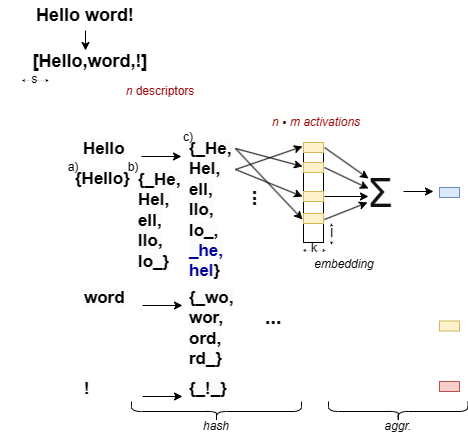
\includegraphics[width=\linewidth]{images/draft/trigram-encoding.png}
% \caption{encode possible cases: a,b,c}
% \label{fig:trigram_encode}
% \end{subfigure}
% \begin{subfigure}{.7\linewidth}
% 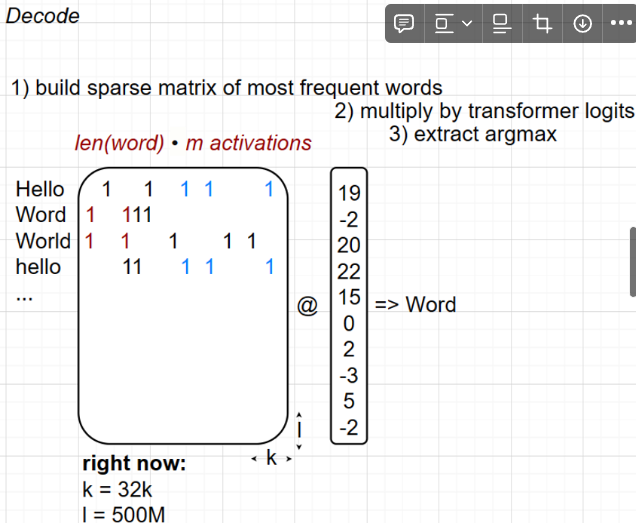
\includegraphics[width=\linewidth]{images/draft/decode.png}
% \caption{``greedy'' decode (argmax)/ training objective  (binary multi-class)}
% \label{fig:decode}
% \end{subfigure}
% \caption{depiction of new tokenization  $s\cdot k$, $s=3, l=4k$}
% \label{fig:trigram}
% \end{figure}

% \begin{figure*}
%     \centering    
%          \dummyfigure{.95\linewidth}{5cm}{Hyp-ablation}
%          \caption{\method~is competitive with classic tokenization approaches on downstream benchmarks. }
%     \label{fig:enter-label}
% \end{figure*}


\begin{figure}
\centering
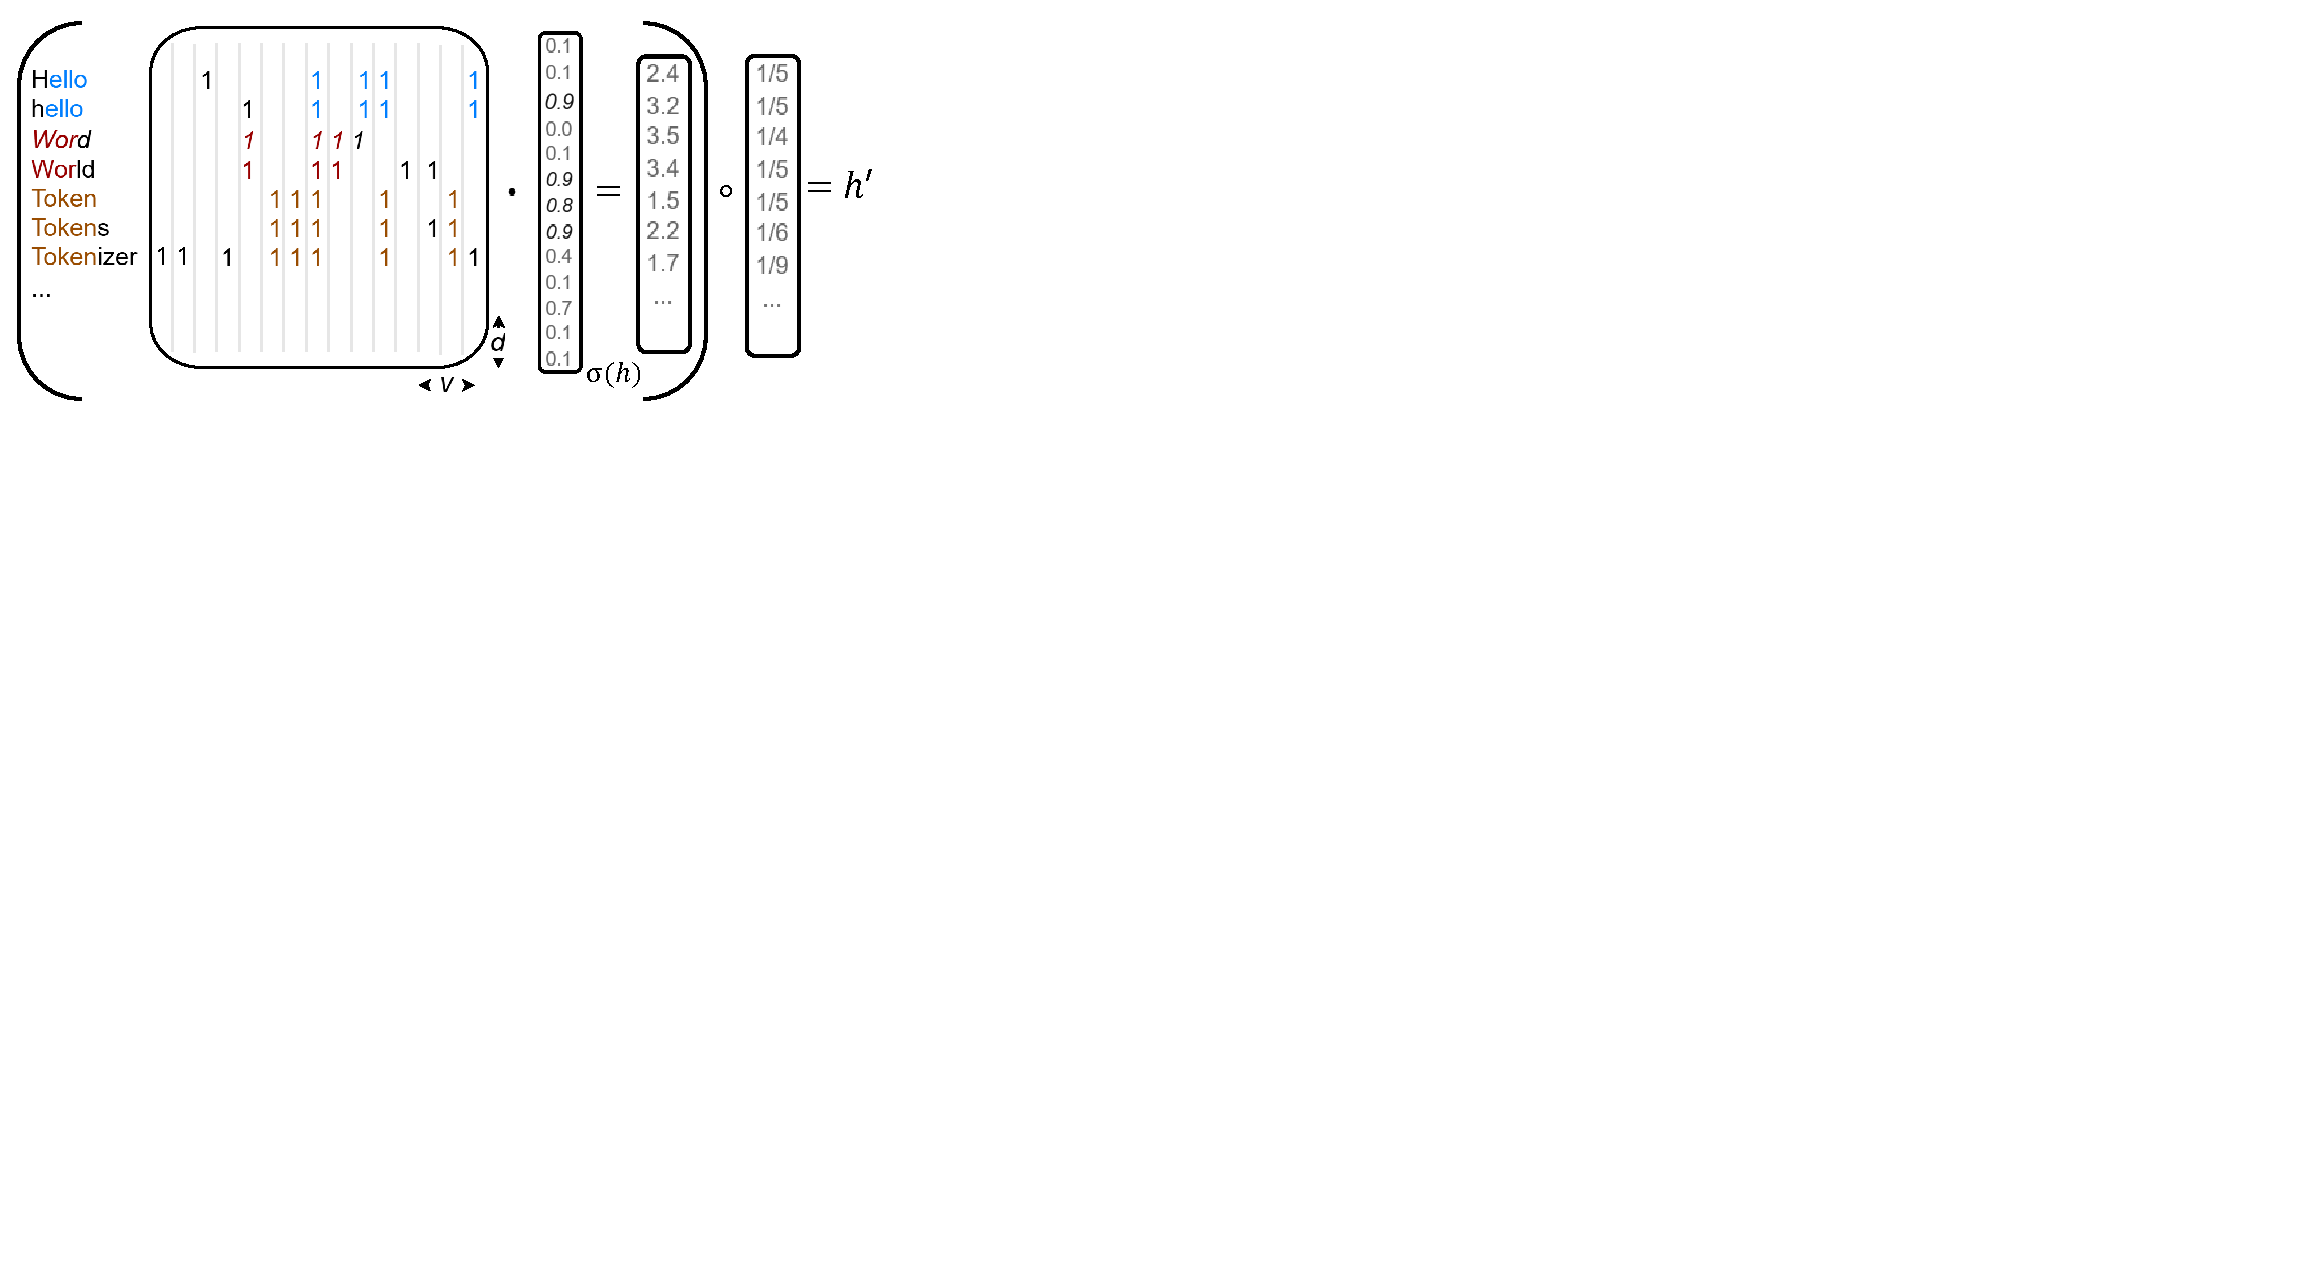
\includegraphics[width=\linewidth,clip,trim={0 15cm 24cm 0}]{images/decoder_short.pdf}
\caption{Example of the next word prediction with \method. To the list of predictable words of dimension $d$ we generate once the corresponding patterns within the available vocabulary size $v$, as described in the encoding step $2$ of Sec.~\ref{sec:encoding}. Note how morphologically close words will generate overlapping patterns. The element-wise sigmoid values of the output of the last hidden layer, $\sigma(h)$, is multiplied with this pattern matrix using standard dot product. Finally, we use $h'$ for the sampling process, the average sigmoid value of a word. C.f. App.~\ref{app:mesa_algo} for further details.}
\label{fig:decode}
\end{figure}

\section{Empirical Evaluations}
% \ps{refer to flaws from section 2, for each state how it is measured}
% We continue to clarify details of our experimental setup. Subsequently, we empirically demonstrate the shortcomings of common tokenizers in contrast to the capabilities of our proposed approach. 
We continue with an empirical demonstration of the performance of \method, and how it remedies the flaws of standard tokenizers as outlined in Sec.~\ref{sec:flaws}.  
To thoroughly analyze the performance differences, we designed three consecutive experiments:
First, we perform hyperparameter ablations on a series of 1B parameter models, which achieve competitive scores on standard benchmarks with a reduced vocabulary, which in turn addresses \textbf{F1}.
Second, we analyze the duplicates in the tokenizers of recent LLMs with respect to \textbf{F2}. 
Notably, \method\ is by design free of duplicates. 
Lastly, we look at \textbf{F3} and evaluate the performance of various tokenizers across languages. Further, we trained 3B parameter models on English and continued training on German data to practically investigate language adaptability.  \method\ has better tokenization performance across languages and outperforms classic tokenizers on language transfer. 


\subsection{Experimental Details}
First, let us clarify some details about our experimental setup. We provide more details for each section in the Appendix.

\textbf{Data and Code.}
We use the slimpajama dataset~\cite{cerebras2023slimpajama} as our English and Occiglot Fineweb v0.5 \cite{brack2024occiglot}
as our German data corpus.
Both datasets contain a diverse range of content and have been extensively filtered and deduplicated. 
% Slimpajama is a cleaned variation of redpajama, as such contains a wide range of samples including arxiv, wikipedia and code, is filtered to contain only English items, and has been validated in previous studies.
% \todo{Occiglot is...}\mb{todo}

As a baseline, we trained BPE and Unigram tokenizers of sizes 32$k$ and 64$k$ on a random 20GB slimpajama sample using Sentencepiece\footnote{\url{https://github.com/google/sentencepiece}}. More details are described in App.~\ref{app:sentencepiece}.

To ensure fair comparisons, we trained 1B and 3B models from scratch for the baselines and \method\ using our adjusted code base\footnote{\url{https://github.com/Aleph-Alpha/trigrams}}.


\begin{figure}
    \centering    
         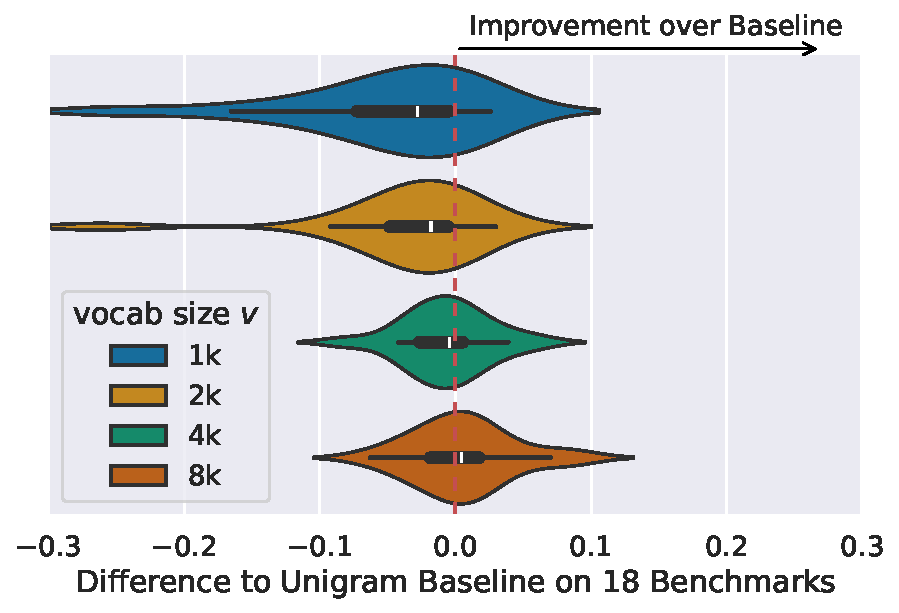
\includegraphics[width=.9\linewidth,height=140px]{images/ablation_hidden_size_upper.pdf}
         \caption{Hyperparameter search for Vocab Size of \method\ on a series of 1B ablations. We fixed number of activations $m=10$, and do not apply lowercase overlap ($k=0$). The boxplots show the differences of trained models to a $64k$ unigram baseline for 18 downstream benchmarks (0-shot). 
         %Albeit with some variance, 
         \method\ outperforms in median the classical tokenizer architecture with a reduced vocab size of $8k$ entries ($12.5\%$).}
    \label{fig:hyperparameter_1b}
    % \vskip -1.em
\end{figure}



\textbf{LLM Pre-Training.}
All models are transformer, decoder-only architectures similar to Llama-2. We solely change the tokenizer, embedding layer and LM head. Consequently, ablations with smaller sizes of $v$ result in a lower overall parameter count, heavily skewing the comparison in \textit{favor of the baseline}. 
For hyper-parameter ablations of \method, we train 1B models for $50k$ steps with $2k$ sequence length and $1k$ total batch size.
We then scale up the baseline and \method\ models to 3B parameters and train for $110k$ steps on slimpajama with $4k$ sequence length. For the multilingual learning experiment, we continue training this English 3B model at a lower learning rate for another $20k$ steps on German Occiglot data with a $20\%$ replay of English.  
%To assess the effects of sparsely aggregated text embeddings on downstream LLM performance, we train and evaluate multiple models and baselines from scratch only ablating the tokenizer and embedding layer. 
%For the hyperparameter sweep of \method, we train a series of 1B transformer models similar to LLama-2 \cite{} with a hidden size of $2048$, using Gelu activations and RMSNorm and $16$ layer. All models are trained on Slimpjama \cite{} for $50k$ steps with $2k$ sequence length and $1k$ batchsize.
% In general, we compare against two baselines: A Unigram tokenizer with 32k and 64k vocabulary sizes and default embedding layer. For our method, we perform ablations over the hyperparameters embedding size $v$, number of activations $m$ and lowercase trigram overlap $k$. 

% For continued pre-training we train a series of 3B models with hidden size of $3072$, $24$ layers, Swiglu MLP, sequence length of $4k$ and are trained for $90k$ steps on slimpajama. Afterwards we lower the learning rate and train on another $20k$ steps on a mixture of $20\%$ redpajama and $80\%$ occiglot data.



\textbf{Evaluation.} 
We evaluate tokenizer performance in isolation using fertility measurements similar to \citet{rust2021howGood}. Fertility benchmarks the number of tokens required per word with $1.0$ thus being the optimal value.
Specifically, we 
%use %UDPipe \cite{} for ground-truth tokenization and 
compare different tokenizers across 5 diverse languages on the respective data from Wikipedia. 

Downstream benchmark comparisons are performed on 18 standardized benchmarks\footnote{\scriptsize\url{https://github.com/EleutherAI/lm-evaluation-harness}} in English that measure a wide variety of LLM capabilities, including general language modeling, question answering, and common sense reasoning. 
%We use the code of the eleuther eval harness, and evaluate each benchmark in 0-shot and 2-shot.
To evaluate german and english in comparison we use german translations of the Hellaswag, Truthfulqa and Arc-Challenge benchmarks\footnote{\url{https://github.com/bjoernpl/GermanBenchmark}}.

We built \method's prediction dictionary, from the top $80k$ words that occurring in slimpajama, and additional top $20k$ words from the German Occiglot data. 
%Since Wikipedia contains an uncharacteristic large amount of numbers (e.g. years) that might distort results, we filtered these out. 
%\todo{appendix? or what exactly is filtered.}
%\todo{one more sentence how udpipe works/ what is measured exactly.}\mb{todo}


%Detailed training parameters are described in App.~\ref{app:training_parameters}.




%\subsection{\ps{what about starting with Fig. 2? So first competitive with baseline, then for each flaw one experiments/subsection/plot to show advantage?}}


\begin{table*}[h]
\small
    \centering
    \begin{tabular}{l | r r r r | r r r r r }
    \multirow{ 2}{*}{\textbf{Model/Tokenizer}} & \multicolumn{4}{ c |}{\textbf{Portion of duplicate tokens (\%) $\downarrow$}} & \multicolumn{5}{ c }{\textbf{Fertility across languages $\downarrow$}}\\
        &  Total & Cap. & Space & Digits & {EN} & {DE} & {RU} &{VI} &{AR}\\ \hline
      Unigram (64k)& 35.24 & 23.27 & 13.47  & 0.00 & 1.280 & 2.004 & 11.431& 5.060 & 9.455 \\
      BPE (64k)& 35.24 & 23.27 & 13.47  & 0.00 & 1.275 & 2.025 &  11.423 & 4.755 & 9.465 \\
      \hline
      Mistral (32k) & 31.47 & 19.10 & 16.45 & 0.00 &  1.397 & 1.931 & 2.560 & 3.346 & 4.722 \\
      Phi-2 (50k) & 23.23 & 12.91 & 16.89 & 3.32 & 1.265  & 2.266 & 6.729 & 4.339 & 5.225 \\
      Gemma (256k) & 34.68 & 20.27 & 20.50 & 0.04 & 1.176 & 1.447 &  1.903 & 1.726 & 1.793 \\
     
      Command-R (255k) & 15.31 & 15.31 & 14.00 & 0.00 & \textbf{1.152} & 1.411 &  1.590 & 1.597 & 1.578 \\
      \hline
      \textbf{\method} (Ours) & \textbf{0.00} & 0.00 & 0.00 & 0.00  &  {1.163} & \textbf{1.182} & \textbf{1.338} & \textbf{1.400} & \textbf{1.086} \\

    \end{tabular}
    \caption{Demonstration of inherent benefits of \method~over traditional tokenizers. The performance no longer degrades when confronted with languages beyond the one primarily trained on. Additionally, the vocabularies of classic tokenizers contain large portions of tokens only differing in their capitalization or leading whitespace. \method~does not construct such a vocabulary in the first place and thus utilizes embeddings more efficiently.}
    \label{tab:language_fertility}
    \vskip 1.em
\end{table*}


\subsection{\method\ performs at 8$k$ vocab size}
We present the results of our hyperparameter ablation study of \method\ for $1B$ models in Fig.~\ref{fig:hyperparameter_1b}. All scores are reported as differences to the Unigram $64k$ baseline and for fixed parameters $m=10$ and $k=0$. 
Generally, \method~remains highly competitive with the baseline as all versions outperform the Unigram model on some of the benchmarks. Further, we achieve the best results for a vocab size $v$ of $8k$ at which \method~outperforms the baseline on average. 
In contrast, a vocab size of $\leq 2k$ seems insufficient with devastating outliers.
%, \todo{and further increasing the size $\geq 16k$ does not result in additional performance}\footnote{Partially due to the undertrained stage of the model.}. 
We performed further ablations on parameters $m$ and $k$, which are outlined in App.~\ref{app:hyperparameter_ablation}. 
%However, their impact on overall model performance remains small compared to vocab size $v$.

These results demonstrate that \method\ successfully addresses the flaw of large vocabularies and embedding layers (\emph{cf.} \textbf{F1} in Sec.~\ref{sec:flaws}).  
We are able to achieve competitive performance with only $12.5\%$\footnote{$8k$ instead of $64k$.} of the embedding parameters  using \method~instead of Unigram. 

Note, that we do not adjust any other model parameters when reducing vocab size. 
As such, the benchmark results compare a Unigram model with $1.07B$ parameter against a \method\ model with $0.84B$ parameters (for $v=8k$). 
 Consequently, we demonstrate that an LLM using \method~instead of Unigram performs better, despite having over 20\% fewer parameters.


% The results of the hyperparameter ablations are summarized in Fig.~\ref{fig:hyperparameter_1b}.
% For fixed $m=10$ and $k=0$, we train a series of $1B$ models with varying vocab size $v$, and display the resulting performance difference to a $64k$ unigram baseline.
% As shown, a vocab size of $8k$ performs on average better than all other ablations. 
% While a vocab size of $\leq 2k$ seems insufficient with devastating outliers, a size $\geq 16k$ apparently does not add value to the capabilities of the model. Cause to the latter may also be the early stop of the model trainings---thery are all are still far from convergence---or overall due to the limited capabilities of $1B$ models. 
% Notably, the resulting   $64k$ tokenizer baseline performs on average worse than \method\ with a reduced vocabulary of $8k$ entries $(12.5\%)$. 

% \mb{Ablations on other hyper parramters}
% Note that we exchange the vocab size while leaving all other parameters fixed. 
% As such, we technically compare a unigram model with $1.07B$ parameters against our \method\ model of $0.84B$ (for $8k$ entries).
% More details of the ablations are outlined in App.~\ref{app:training_parameters},.
% \mb{\textbf{F1)}}





% \begin{figure}
%     \centering
   
% 
\includegraphics[width=.95\linewidth,clip,trim={0 7cm 0 0}]{images/plot_de_en_avg_v2.pdf}
%          \caption{3B Continual pre-training on german}
%     \label{fig:continual_3b_german}
%     \end{figure}
% \begin{table*}
% \centering
% \begin{tabular}{c|c||c|c||c|c||c|c||c}
%     % & &  &  & stage 1 & stage 2\\
%    size &approach & embedding & model & eval (1) & eval (2) & fertility&overlap & runtime\\
%     \hline
%     \parbox[t]{1mm}{\multirow{5}{*}{\rotatebox[origin=c]{90}{1Billion}}} 
%     &ours & $2\times \textbf{16M}$ & XM & \textbf{x/0} & \textbf{x/x}& \textbf{x/x}&\textbf{0/0}& \\
%      &unigram (32k) & $2\times 128M$ & XM & x/0 & x/x & x/x & x/x&\\
%     &unigram (64k) & $2\times 256M$ & XM & x/0 & x/x & x/x & x/x&\\
%      &bpe (32k) & $2\times 128M$ & XM & x/0 & x/x & x/x& x/x&\\
%     &bpe (64k) & $2\times 256M$ & XM & x/0 & x/x & x/x& x/x&\\
%     \hline
%     8B &llama3$^*$ & 1/8 & 7/8 & & - &  &\\
%     XB &gemma$^*$ & & & & - && \\
%     101B &cohere R$^*$ & 6B (6/101\%) & 95/101\% & & - && \\
%     8B &Aya$^*$ & 1/8\% & 7/8\% & & - && \\
%     35B &Aya$^*$ & 2/35 & 33/35 & & - &&
% \end{tabular}
% \caption{\todo{Note: 1B trained Xk slimpajama eval (1) and continued for xk german data (2). $^*$ not trained at all -> only 1 eval. all scores are english/german. embeddings affects $\times 2$: embed + lm head }}
% \end{table*}




\subsection{\method\ no duplicates by design}
\label{sec:exp_flaws}
Let us now look into (near) duplicate tokens  in commonly used tokenizers (\emph{cf.} \textbf{F2} in Sec.~\ref{sec:flaws}). In general, there are three types of overlaps in vocabularies: 1) The same token with and without capitalization, 2) with and without leading whitespace, and 3) dedicated tokens for multiple digits. 

In Tab.~\ref{tab:language_fertility}, we report the percentage of duplicate tokens for our baseline tokenizers and commonly used models. Overall, between 15\% and 35\% of the available vocabulary is spent on (near) duplicate information with limited differences in entropy. Generally, tokenizers contain the most duplicates for capitalization, slightly fewer for whitespaces, and only a few duplicate digits. The relative amount of overlap tends to decrease with larger vocabularies, although Gemma marks an inglorious exception.
In contrast, \method~is inherently designed to be free of duplicates.
We can even adjust the parameter $k$ to explicitly model the overlap of words to their lowercase representations. Consequently, all variants are inherently well represented in the emedding layer. 
%As we demonstrate in the next section, these design choices \todo{lead to smoother training loss curves} and improved downstream performances.

\subsection{\method\ has lower fertility across, \mbox{and is more adaptive to new languages}}
\label{sec:main_results}

Finally, we investigate the versatility of tokenizers beyond their (main) language (\emph{cf.} \textbf{F3} in Sec.~\ref{sec:flaws}). We report the fertility of our baselines and other popular models in English, German, and three dissimilar languages that also contain significant character-level differences in Tab.~\ref{tab:language_fertility}. Common to all tokenizers is a significantly decreasing performance for non-English languages, especially for Russian and Vietnamese. Naturally, larger vocabulary sizes tend to have better multilingual coverage
%(if they were explicitly present in the reference corpus)
, in particular to language groups close to English, but still suffer from significant performance drops. 
In comparison, the tokenization of \method, which is mainly based on whitespace splitting, provides comparably good performance across all $5$ languages\footnote{More detailed evaluations are found in App.~\ref{app:fertility}.}. The increases in fertility for Russian or Vietnamese remain small and there is no performance difference for German or Arabic. 
Note that these synergies were explicitly modeled, and no reference corpus is needed to train and bias the fertility of \method.
Consequently, \method~allows for easier and more efficient model adaptation to low-resource languages. 


We now explicitly show the devastating consequences of biased tokenizers on the language transfer capabilities of LLMs. 
As discussed above, we first train $3B$ models for \method~and Unigram on English, and then transition to German.
Through more ablations, we fixed the activations to $m=7$ and the lowercase trigram overlap to $k=3$.
Fig.~\ref{fig:continual_3b_german} shows the performance average on the English and German versions of the standard benchmarks.
The baseline performance in German is already improved with \method, indicating that syntactic and semantic similarities between the languages are better captured in the learned representations.
Additionally,  \method\ almost achieves the English-level performance on German after $20k$ training steps. In contrast, the classical tokenizer variant improves only marginally with the same amount of training.

We, again, do not adjust any other model parameters when reducing the vocab size. 
As such, \method~uses 10\% fewer parameters than the baseline ($2.77B$ instead of $3.11B$) and still strongly outperforms the Unigram variant. More detailed evaluations are found in App.~\ref{app:benchmarks}.


\begin{figure}
    \centering    
         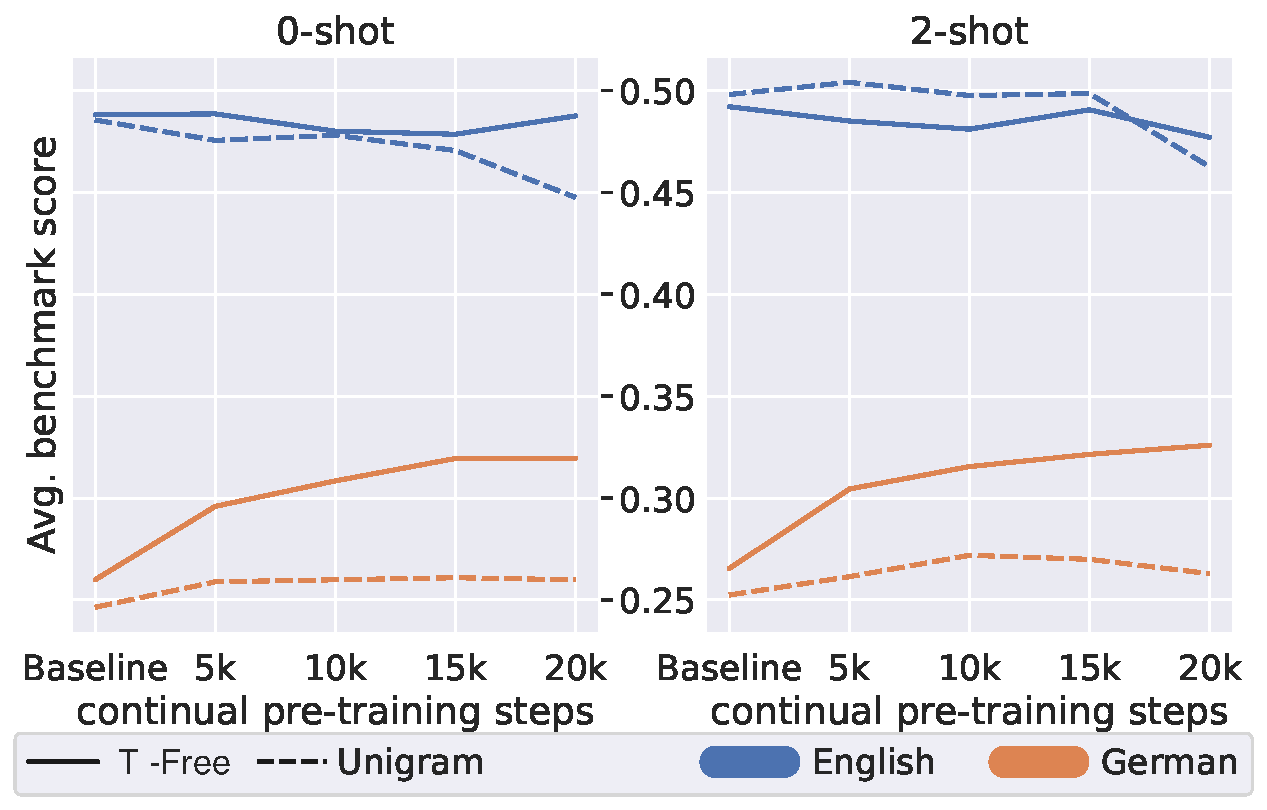
\includegraphics[width=\linewidth]{images/plot_de_en_avg_v2_v2_t.pdf}
         \caption{Continual pre-training performance. Trained are $3B$ models on English slimpajama data for $90k$ steps (``baseline''), and continued on German occiglot data for $20k$ steps. Plotted are the average scores of two benchmarks available in German and English: Hellaswag and Arc-Challenge. Notably, \method\ outperforms in German already with the baseline. Within $20k$ continued steps, \method\ improves by $5\%$ on average in 0 and 2-shot, while the classic tokenizer approach barely improves. Both models slightly drop performance in English, albeit the tokenizer version more drastically. Full evaluations are found in Appendix Tab.~\ref{tab:evalende},\ref{tab:evalen1},\ref{tab:evalen2}.}
    \label{fig:continual_3b_german}
    % \vskip -1em
\end{figure}
\section{Discussion}
\label{sec:discussion}
Prior research has demonstrated that the mapping into a sparse hidden representation and the training of a dense aggregation layer as applied in \method, is a universal function approximator \cite{cmac}. These results provide further theoretical motivation for our approach. 




 \method\ allows for significant compression of an LLMs' vocabulary by more than 85\% without performance degradation. 
 Notably, the affected embedding and head layers are by far the largest in LLMs in terms of parameter count. They are also the most influential to an LLM, as they dictate the mapping between text and numerical representations. For one, these massive improvements allow for better utilization of billions of parameters in large models.
 The compression of \method~in particular paves the way to building better low-resource models, by reducing model size and training cost and improving adaptability. 
 For example, in our experiments without pipe or model-parallelism, we were able to \emph{triple} the micro-batch size, yielding faster training iterations.
 
%  Notably, the affected embedding and head layers are the biggest ones (each \emph{hidden size $\times$ vocab size}) occurring in a language model and can themselves already span billions of parameters. The deployment of \method as such paves the way for new low-resource SOTA models. The reduction of the biggest matrices are in particular beneficial to reduce training costs. As the multiple billion parameters are further duplicated during loss and gradient computations, they would need special sharding or iterated computation techniques to fit on a GPUs memory.
% With \method\ we were able to triple the micro batchsize and as such speed up training, without implementing any further optimization techniques.

Furthermore, we observed more stable loss curves for \method, in particular for higher learning rates. These improvements may be attributed to the explicit modeling of similar words, the removal of duplicates, and the less volatile multi-label training target.
Further, the uniform hashing distributes gradients evenly amongst the available vocab size, in contrast to classical approaches.
We provide further details in App.~\ref{app:training_parameters},\ref{app:training_stability}.

%The methodology behind \method\ also results in further benefits. 
The rules we use for obtaining word representations are universal and well-defined at pre-training time. They do not change over time, particularly neither when adding languages later on.
%In fact, it resembles a form of byte-aggregations into a single embedding in the style of convolutions.
\method\ also lowers computational costs due to its low fertility and easy-to-process whitespace splitting. Consequently, pre-processing, training and inference of an LLM all require less compute. 
% Note that the proposed method simplifies the computational resources, i.p., it lowers the text fertility, i.e. the number of processing steps in training and inference.
% Moreover, the actual tokenization process is simplified to a whitespace split, which in particular saves a lot of (CPU-) resources when tokenizing large documents (e.g. ``books'' dataset) that takes already hours with a unigram tokenizer of $128k$ vocab size.  

Lastly, \method\ allows to explicitly model and steer the decoding process at inference time, by altering the available dictionary. 
%Recall that the dictionary is precomputed and includes all possible predictable words. 
Consequently, hallucinations will likely be reduced due to fewer ``generic fall-back'' word splits. Moreover, one can dynamically add or remove words. 
It is worth pointing out that \method's compression benefits can also be combined with traditional tokenizers. Instead of the simple whitespace splitting one could keep traditional tokenization and trigramify ``classic tokens''. 
%We leave detailed analysis of this direction to future research.
% On the other hand, to continue on a preferred tokenizer performance (e.g. depending on these generic fall-backs), with the benefit of a compressed embedding layer, one could apply \method\ on each text-split produced by a tokenizer. 



\section{Related Work}

Few alternatives to BPE and Unigram have been found in recent LLMs and research. 
\citet{charformer} propose a gradient-based trainable tokenization module in contrast the otherwise statistical based approach.

The naive approach of splitting the input text into bytes or characters maximizes fertility and thus increases computational requirements. 
\citet{megabyte} employ a mix of multiple models to improve this drawback of byte-wise processing. I.p. they introduce a fixed character-embedding aggregation and a second character-decoder model. However, they use a fixed byte-width that is processed at once, which is not aligned with word splits. 

%In particular, it significantly reduces the size of actual processable text through a NLP model, as the number of processable tokens in current LLMs is still limited.
Consequently, prior research has proposed methods for merging bytes, e.g., through state-space models \cite{wang2024mambabyte}.  However, these approaches still result in performance degradation. 
Finally, linguistically motivated approaches have built tokenizers based on known morphological rules \cite{jabbar2024morphpiece}. However, these methods are usually tailored to specific applications and are usually too costly and error-prone for large, general-purpose models.

\citet{fasttext} in particular discusses how adding subword informations, such as trigrams, enriches the encoding of words and leads to reliable compressions. \citet{hashembed} conduct research on the overloading of different hashfunctions to further improve and compress embedding representations. \citet{hashformer} train BERT-style encoder models based on a different set of hashes on words. \citet{canine} propose a multistage encoding scheme that uses hash functions and convolutions to enhance the BERT-encodings of words.


Another line of work to reduce the vocabulary parameter count is the utilization of weight tying, effectively halving it, as  the embedding and head layers become ``tied'' to the same matrix  \cite{press2017using}. 
However, the effects on performance are still not sufficiently explored, and it arguably imposes a more difficult training objective. 
%However, as degraded performance was experienced and with the recently increased compute memory, most works discontinued this approach.

%\todo{linguistic/morphological tokenizer (take rel work from https://arxiv.org/abs/2307.07262)}

\section{Conclusion}
\label{sec:conclusion}
In this work we present \method, an alternative to subword tokenizers with a simple and explicitly modeled robust hash function on words. It removes the need and pitfalls to limit ``a models potential'' to a ``pre-pre-trained'' vocabulary.
We, moreover, fundamentally shift the established target of training language models, previously designed as a single-label problem, into a multi-label prediction based on word similarities.
Similarities in particular include leading whitespaces and uppercase variations, for which subword tokenizers add specific tokens that are independently trained from scratch.
These contributions allow us to train language models more robust, more adaptable when continuing pre-training with a new language, and with a significantly (to 12.5\%) reduced parameter size without a decrease in benchmark scores. Due to the special role of the matrices, the latter in particular allows one to increase micro-batchsize, which further accelerates training time.
Finally, the consequent convolution-like encoding achieves SOTA fertility scores across most languages and enables by design synergies to similar language groups.
We demonstrated the latter showing that our $3B$ almost achieved ``native-language'' performance after a small amount of language-transfer training steps, in contrast to the tokenizer baseline.


\section*{Limitations}

With \method\ we propose a fundamentally different approach to text encoding and decoding in LLMs.
Due to the intense resources required to train LLMs, we have focused on evaluating models up to $3B$ parameters. Evaluations on even larger models and training datasets remain a relevant point of investigation for future work. Nonetheless, we observed an easy transfer from $1B$ to $3B$ parameters, and we will continue to train and release more advanced models.

We expect \method\ to experience some numerical instabilities for very long words since single-word embeddings are calculated as the sum of their $n \cdot m$ activations. However, less than $2\%$ of the entire slimpajama dataset contains words with more than $10$ characters (\emph{cf.} App.~\ref{app:statistics}), and we did not encounter any issues with the benchmarks. Consequently, such potential instabilities remain statistically insignificant.
Nonetheless, we could adequately tackle long outliers with an additional split rule based on the words length or at the occurrence of repetitions. Subword tokenizers already demonstrate that such approaches will work, even when tokens are at first glance meaningless and underutilized---and again, these cases remain outliers. Moreover, a hybrid setup utilizing a large tokenizer (>512k tokens) with \method~for optimized memory footprint is depicted in Figure~\ref{fig:hybrid}.

Similarly, we did not thoroughly study the effect of repetitive trigrams in words. These did also not occur frequently enough to have any measurable effect on our experiments. As of now, we only accumulate a word pattern in a binary fashion, not accounting for trigrams appearing multiple times in a single word.
%---and would need to count them instead (if that entropy is really needed), which renders decoding more complicated, in particular when choosing between words with one or multiple occurrences. 
As a fallback, one could again, split words at the position of repetitions. Another promising direction would overload embeddings with positional encodings similar to rotary~\cite{rotary}. 


Although \method's fertility on code is on par with that of LLama2 (\emph{cf.} App.~\ref{app:fertility}), it could be further improved by explicitly modeling code patterns. In this work, we have focused on natural language and leave detailed evaluations of \method\ in downstream coding tasks for future research.
Furthermore, we did not investigate languages entirely relying on Unicode byte-encodings, such as Chinese. However, as they seemingly work out-of-the-box with subword tokenizers, we do not expect issues here by splitting them character/ word-wise. In particular for asian symbols, additionally translating the symbols to its romanization through the phonetic alphabet such as pinyin may further improve the synergies of word encodings. 

% The fundamental issue of out-of-vocabulary hallucinations somewhat remains, but should be shifted into predicting similar words, and more explicitly be controllable. This should further be studied.  

Finally, we only studied a single constructed hash function for \method. As this work paves the way to model required language features more explicitly, we are looking forward to variations of the proposed \method~method.

% \section{Societal Impact}
% \mb{This paper presents work whose goal is to advance the field of Machine Learning. There are many potential societal consequences of our work, none which we feel must be specifically highlighted here.}

\section*{Acknowledgments}

% We thank the three anonymous referees for their constructive comments and suggestions, which helped us to improve this paper considerably.

% Kristian
We gratefully acknowledge support by the German Center for Artificial Intelligence (DFKI) project “SAINT”,
the Hessian Ministry of Higher Education, the Research and the Arts (HMWK) cluster projects
“The Adaptive Mind” and “The Third Wave of AI”, and the ICT-48 Network of AI Research Excellence Center “TAILOR” (EU Horizon 2020, GA No 952215). 

% We thank Graphcore, Jamie Packer, Manuel Brack and Samuel Weinbach for the fruitful discussions and the invaluable feedback throughout this work.



% \newpage



\bibliography{references}



\clearpage

\appendix

\section*{Appendix}



\section{\method\ Algorithm}
\label{app:mesa_algo}
Alg.~\ref{alg:split},\ref{alg:mesa_algo},\ref{alg:encode},\ref{alg:dict},\ref{alg:decode} show the core steps to encode text into embeddings, and decode text from model predictions with \method.
Here, \emph{regex.split} denotes an algorithm that splits text based on a regular expression, \emph{hash} denotes an arbitrary hash function like \emph{md5}, $\%$ denotes the mathematical \texttt{modulo} operation.
In style of python, $f'\{token\}\_'$ denotes text formatting to indicate the string with content of variable \emph{token} being followed by an underscore, and $EL[i]$ denotes the $i-$th entry of matrix $EL$ and $'string'[i:i+3]$ three consecutive characters in the text \emph{string} starting from position $i$, where $'s'$ is at position $0$.
Finally, $v\approx 8,000$ is the chosen vocabulary size,
$d\approx 100,000$ is the chosen dictionary size, $h\approx 3,072$ the LLMs hidden size. 
Finally, $\mathbb{0}^h$ denotes a zero vector of dimension $h$ and $\mathbb{1}^{v\times d}$ a matrix with entries $0$ or $1$.
Note that we included some normalization steps in Alg.~\ref{alg:decode}, which we surprisingly found not beneficial for Alg.~\ref{alg:encode} in our ablations.

Finally, refer to Figure.~\ref{fig:llm_pipeline},\ref{fig:decoder} for a step-wise comparison of the computation step, parameters and runtimes. Figure~\ref{fig:hybrid} shows a ``hybrid'' mode, in which embody a classical subword-tokenizer as a text preprocessing step, but utilize \method~to keep the ``tokenizer free LLM backbone''. Arguably, this approach benefits from a compressed embedding layer, and the tokenizer may easier be exchanged afterwards---the encoding of the text-chunks in the backbone will be kept as proposed.

\begin{algorithm}[h]
\caption{token\_split}\label{alg:split}\label{alg:mesa_algo}\label{alg:mesa_algo_decode}
\begin{algorithmic}
% \DontPrintSemicolon
\State \textbf{input:} \emph{text} \vspace{4px}
\State $\textrm{tokens}\gets \textrm{regex.split}((\_|\backslash W|\backslash d), text)$
\State \emph{(cf. Sec.~\ref{sec:whitespace} if necessary)}\vspace{4px}
\State \textbf{output:} \emph{tokens}
\end{algorithmic}
\end{algorithm}

\begin{algorithm}[h]
\caption{trigramify}\label{alg:trigramify}\label{alg:mesa_algo}\label{alg:mesa_algo_decode}
\begin{algorithmic}
\State \textbf{input:} \emph{token, k, m} \\
\Comment{$k:$ lowercase activation, $m:$ total activation} \vspace{4px}
\State $pattern \gets \mathbb{0}^{v}$
\For{$l\in [0,len(token)-1]$}
\State $trigram \gets f'\_\{token\}\_'[l:l+3]$
\For{$i \in [1,m]$}
\If{$i \leq k$}
\State $string_i = \textrm{lower}(trigram)$
\Else
\State $string_i = trigram$
\EndIf
\State $hash_i = \textrm{hash}(f'\{string_i\}\_\{i\}')$
\State $pattern[hash_i\%v] = 1$
\EndFor\vspace{4px}
\EndFor\vspace{4px}
\State \textbf{output:} \emph{pattern}
\end{algorithmic}
\end{algorithm}





\begin{algorithm}[h]
\caption{encode}\label{alg:encode}
\begin{algorithmic}
% \DontPrintSemicolon
\State \textbf{input:} \emph{token}, \emph{EL}\\
\Comment{\emph{EL}: Embedding Layer ($\in \mathbb{R}^{v \times h}$)\phantom{abdcdef}}\vspace{4px}
\State $embedding \gets \mathbb{0}^{h}$
\State $pattern \gets \textrm{trigramify}(token)$
\For{$i\in [0,v-1]$}
\If{$pattern[i] == 1$}
\State $embedding \gets embedding+EL[i]$
\EndIf
\EndFor
\State \textbf{output:} \emph{embedding}
\end{algorithmic}
\end{algorithm}


\begin{algorithm}[h]
\caption{compile\_dictionary}\label{alg:dict}
\begin{algorithmic}
% \DontPrintSemicolon
\State \textbf{input:} \emph{tokens}\vspace{4px}
\Comment{$d$ target tokens} 
\State $dict \gets \mathbb{0}^{d\times v}$
\For{$i\in [0,d-1]$}
\State $dict[i] \gets \textrm{trigramify}(tokens[i])$
\EndFor
\State \textbf{output:} \emph{dict}
\end{algorithmic}
\end{algorithm}


\begin{algorithm}[h!]
\caption{decode}\label{alg:decode}
\begin{algorithmic}
% \DontPrintSemicolon
\State \textbf{input:} \emph{logit}, \emph{dict}, \emph{tokens}\\
\Comment{\emph{logit}: single prediction ($\in \mathbb{R}^{v\times 1}$),\phantom{abcdefg}\\
\phantom{>bcdef}\emph{dict}: compiled dictionary ($\in \mathbb{1}^{d\times v}$),\\
\phantom{>bcdef}\emph{tokens}: $d$ tokens corresponding to \emph{dict} }\vspace{4px}
\State $scores \gets dict \cdot \textrm{sigmoid}(logit)$
\For{$i\in [0,d-1]$}
\State $scores[i] \gets scores[i]/\textrm{sum}(dict[i])$
\EndFor
\State $scores \gets \textrm{softmax}(scores)$
\State $i \gets \arg\max_l\ scores[l]$\vspace{4px}
\State \textbf{output:} \emph{tokens[i]}, \emph{scores[i]}
\end{algorithmic}
\end{algorithm}


\section{Whitespace encoding}
\label{sec:whitespace}
By default our model is trained to predict full words separated by whitespaces. To not be limited to this use-case, we add a special ``non-whitespace'' and ``whitespace'' token. We empirically evaluated each exception occuring in code tokenization.
To further reduce its fertility, we favor ``non-whitespace'' before one of the following characters:
\begin{lstlisting}
$.,;:#?!=-+*/\()<>[]&@%_~^
\end{lstlisting}
We further prefer non-whitespace after one of the following characters:
\begin{lstlisting}
#$=-+*/'\"(<[~^&@%_\n1234567890
\end{lstlisting}

As such, the text ``In 2024'' would result in the split ``[In,2,0,2,4]'' without the need of any special annotations, while ``In20 24'' resolves to ``[In,<no\_ws>,2,0,<ws>,2,4]''.

Finally, to further improve code fertility, we merge consecutive <ws> and newline tokens up to 3 times, i.e. $8$ consecutive whitespaces would result in a single <|8<ws>|> token.


\section{Tokenizer trainings with sentencepiece}
\label{app:sentencepiece}

For training of a unigram tokenizer with the current sentencepiece library, a 20GB reference data corpus reaches the limit of our available 1TB Ram compute node.
We thus randomly sample 20GB of the slimpajama dataset and run the following statement for training of the actual tokenizer: 
\begin{lstlisting}
spm_train --input=20GB_sample.txt\
--model_prefix=unigram_64k \
--vocab_size=64000 \
--character_coverage=0.99 \
--model_type=unigram \
--byte_fallback=true \
--split_by_number=true  \
--split_by_whitespace=true  \
--train_extremely_large_corpus=true\
--split_digits=true  \
--allow_whitespace_only_pieces=true\
--remove_extra_whitespaces=false \
--normalization_rule_name=nfkc \
--num_threads 64 --eos_id=0 \
--bos_id=-1   --unk_id=2 \
--pad_id=1 \
--eos_piece="<|endoftext|>" \
--pad_piece="<|padding|>" \
--unk_piece="<|unknown|>"
\end{lstlisting}

\section{Training Configurations}
\label{app:training_parameters}
\subsection{1B}
Training Parameters are listed in Tab.~\ref{tab:1b_parameters}.

\begin{table}[]
    \centering
\begin{tabular}{lrr}
\toprule
         Parameter & Value \\
\midrule
hidden size & 2,048 \\
layers &  16 \\
attention heads & 16 \\
norm & layer \\
mlp & gelu \\
mlp scale & 5,456 \\
training steps & 50k \\
sequence length & 2,048 \\
batch size & 1,024 \\
\midrule
precision & bfloat16 \\
learning rate &  6e-4 \\
minimum learning rate & 6e-5 \\
annealing & cosine \\
annealing steps & 50k \\
warmup steps & 200 \\
optimizer & AdamW \\
optimizer beta1/ beta2/ eps & 0.9 / 0.95 / 1e-8 \\
weight decay & 0.1 \\
\bottomrule
    \end{tabular}
    \caption{1B Parameter configurations (for all ablations).}
    \label{tab:1b_parameters}
\end{table}

\subsection{3B}
Training Parameters are listed in Tab.~\ref{tab:3b_parameters}.

\begin{table}[]
    \centering
\begin{tabular}{lrr}
\toprule
         Parameter & Value \\
\midrule
hidden size & 3,072 \\
layers &  24 \\
attention heads & 24 \\
norm & rms \\
mlp & swilu \\
mlp scale & 8,192 \\
training steps & 90k (20k) \\
sequence length & 4,096 \\
batch size & 1,024 \\
\midrule
precision & bfloat16 \\
learning rate &  3e-4 (1e-4) \\
minimum learning rate & 3e-5 (3e-5)\\
annealing & cosine \\
annealing steps & 90k (20k) \\
warmup steps & 200 (500) \\
optimizer & AdamW \\
optimizer beta1/ beta2/ eps & 0.9 / 0.95 / 1e-8 \\
weight decay & 0.1 \\
\bottomrule
    \end{tabular}
    \caption{3B Parameter configurations (for all ablations). In brackets are highlighted values for German continued pre-training.}
    \label{tab:3b_parameters}
\end{table}


\section{Fertility Analysis}
\label{app:fertility}
We subsequently provide further experimental details on the fertility analysis conducted with respect to \textbf{F3}, Sec.~\ref{sec:main_results}. 
As a reference dataset, we used the November 23 dump of Wikipedia in the respective languages. We derived reference tokenization using UDPipe \cite{straka-2018-udpipe}. A tokenizer's fertility is then calculated by dividing its total token count for a document by the number of tokens produced by UDPipe.
We present results for more models on 8 languages in Tab.~\ref{tab:language_fertility_complete}.

We also evaluated the white-space tokenization of \method\ for code. For 22 programming languages, we took 10k random documents each from the starcoder dataset \footnote{\url{https://huggingface.co/datasets/bigcode/starcoderdata}}. Since ground truth text splitting for code is hard to establish, we instead report the normalized sequence length with respect to a reference tokenizer. We here used Llama-2 and report results in
Tab.~\ref{tab:code_nsl}. Since \method's tokenization achieves an NSL close to $1.0$, it performs roughly on par with Llama-2.
\section{Token Overlap/Duplicates}
For the empirical evaluation regarding \textbf{F2}, \emph{cf.} Sec.~\ref{sec:exp_flaws}, we present more exhaustive results with additional models in 
Tab.~\ref{tab:token_overlaps}.
 
\begin{table}[]
    \centering
\begin{tabular}{lrr}
\toprule
     lang & Ours (NSL) $\downarrow$ &  Starcoder (NSL)  $\downarrow$\\
\midrule
    c-sharp &  1.034783 &   0.816206 \\
          c &  0.996308 &   0.860453 \\
        cpp &  1.084867 &   0.855094 \\
        css &  1.109492 &   0.903693 \\
       cuda &  1.018222 &   0.857034 \\
 dockerfile &  0.954086 &   0.851568 \\
         go &  1.142476 &   0.883456 \\
       html &  1.164936 &   0.885237 \\
       java &  1.003201 &   0.835858 \\
 javascript &  1.183923 &   0.850398 \\
       json &  1.071685 &   0.892871 \\
     kotlin &  0.925868 &   0.846053 \\
   makefile &  1.006108 &   0.862994 \\
   markdown &  0.965325 &   0.892784 \\
        php &  1.179374 &   0.838566 \\
     python &  1.005064 &   0.857439 \\
       ruby &  0.979135 &   0.846597 \\
       rust &  1.086027 &   0.857645 \\
      shell &  1.041322 &   0.879112 \\
        sql &  0.954786 &   0.859785 \\
 typescript &  1.121119 &   0.847393 \\
       yaml &  0.974146 &   0.856218 \\

\textbf{Overall} & 1.045557 & 0.860748 \\
\bottomrule
\end{tabular}
    \caption{Normalized sequence length wrt Llama-2 on code tokenization.}
\label{tab:code_nsl}
\end{table}



\begin{table*}[]
\small
    \centering
    \begin{tabular}{l | r r r r r r r r}
     \textbf{Model}    &  \textbf{EN} & \textbf{DE} & \textbf{FR} & \textbf{ES} & \textbf{IT} & \textbf{RU} &\textbf{VI} &\textbf{AR} \\
     \hline
      
      Unigram Baseline (32k) & 1.3584 & 2.2577  & 2.1354 & 2.1524 & 1.9508  & 11.4448 & 5.1826 & 9.4740\\
      Unigram Baseline (64k) & 1.2802 & 2.0043 & 1.9492 & 1.9163  & 1.7263 & 11.4305& 5.0603 & 9.4555\\
      BPE Baseline (32k) & 1.3585 & 2.2784  & 2.0625 & 2.0977 & 1.9396 & 11.4321 & 4.8717 & 9.4694\\
      BPE Baseline (64k) & 1.2759 & 2.0253 & 1.9059 & 1.8894 & 1.7212 & 11.4231 & 4.7545 & 9.4656\\
      Mistral (32k) &  1.3973 & 1.9316 & 1.6613 & 1.7569 & 1.7591 &  2.5601 & 3.3458 & 4.7228\\
      Llama-2 (32k) & 1.4014 & 1.7702 & 1.5495 & 1.6413 & 1.6160 & 2.3242 & 3.3540 & 4.8255\\
      Phi-2: (50k) & 1.2654  & 2.2660 & 1.8183 & 1.9736 & 1.9132 & 6.7289 & 4.3392 & 5.2246\\
      Gemma (256k) & 1.1761 & 1.4470 & 1.2754 & 1.3163 & 1.3253 & 1.9028 & 1.7257 & 1.7938\\
      DBRX (100k) & 1.2381 & 1.8311 & 1.5423 & 1.6142 & 1.6191 & 3.2385 & 2.6617 & 3.6821\\
      Jais (85k) & 1.3029 & 2.1391 & 1.7347 & 1.8514 &  1.8244 & 3.6730 & 3.4382 & 1.2653 \\
      Command-R (255k) & \textbf{1.1525$\bullet$} & 1.4110 & 1.2079 & 1.2527 & 1.2460 & 1.5899 & 1.5967 & 1.5787\\
      Llama-3 (128k) & 1.2330 & 1.8221 & 1.5351 & 1.6033 & 1.6130 & 2.2144 & 1.8261 & 1.9660\\
      NeMo-Tekken (131k) & 1.2313 & 1.5178 & 1.3061 & 1.3845 &  1.4171 & 2.0521 & 1.8378 & 1.6045 \\
      \textbf{Ours}   &  \textbf{1.1636$\circ$} & \textbf{1.1829} & \textbf{1.2363} & \textbf{1.1695} & \textbf{1.1274} & \textbf{1.3386} & \textbf{1.4001} & \textbf{1.0863}\\

    \end{tabular}
    \caption{Additional evaluations of fertility evaluations. \emph{Cf.} Sec.~\ref{sec:exp_flaws}.}
    \label{tab:language_fertility_complete}
\end{table*}



\begin{table*}[]
     \small
    \centering
    \begin{tabular}{l | c r r r|}

    \multirow{2}{*}{\textbf{Model/Tokenizer}} & \multicolumn{4}{ c |}{\textbf{Portion of duplicate tokens (\%) $\downarrow$}}\\
         &  \textbf{Total} &\textbf{Cap.}  &  \textbf{Space} & \textbf{Digits}\\
     \hline
      Unigram Baseline (32k) & 32.99 & 21.44 & 11.76 & 0.00\\
      Unigram Baseline (64k) & 35.24 & 23.27 & 13.47  & 0.00\\
      BPE Baseline (32k) & 32.12 & 21.30 & 13.85 & 0.00\\
      BPE Baseline (64k) & 35.32 & 23.82 & 15.52  & 0.00\\
      Phi-2: (50k) & 23.23 & 12.91 & 16.89 & 3.32\\
      DBRX (100k) & 24.87 & 23.77 & 16.17 & 1.10\\
      GPT-2 (50k) & 25.25 & 21.93 & 16.99 & 3.32\\
      Gemma (256k) & 34.68 & 20.27 & 20.50 & 0.04\\
      Command-R (255k) & 15.31 & 15.31 & 14.00 & 0.00\\
      Mistral (32k) & 31.47 & 19.10 & 16.45 & 0.00\\
      Llama-2 (32k) & 30.23 & 17.10 & 16.98 & 0.00\\
      Llama-3 (128k) & 21.22 & 20.17 & 15.28 & 1.05\\
      NeMo-Tekken (131k) & 23.12 & 13.30 & 11.99 & 0.00\\
      \textbf{T-Free} (Ours) & \textbf{0} & \textbf{0} & \textbf{0} & \textbf{0}\\
    \end{tabular}
    \caption{Additional evaluations of overlap of full tokens occuring multiple times, only with capitalization or whitespace in difference. Note that there are still plenty more redundancies with sub-token reconstructions. \emph{Cf.} Sec.~\ref{sec:exp_flaws}.}

    \label{tab:token_overlaps}
\end{table*}



\section{Training stability}
\label{app:training_stability}
Memory footage comparing classic tokenizers to \method\ is found in Fig.~\ref{fig:memory_footprint}.

Note that the hashing step of Alg.~\ref{alg:trigramify} uniformly distributes gradients amongst the available vocabulary, as discussed in Sec.~\ref{sec:discussion}.
This is in contrast to classic tokenizers, as they depend on a bijective single-label mapping, and as such each vocabulary entry update is dependent on its the occurance frequency of the corresponding token within the dataset.
Moreover, we explicitly let trigram activations overlap with their lowercase version. We assume that these are responsible for the more stable training dynamics as shown in Fig.~\ref{fig:training_loss}.
Moreover, we found that the lowercase overlap bootstraps learning as shown with the downstream benchmark ablations Fig.~\ref{fig:hyperparameter_ablation}. 

    
\begin{figure*}
    \centering
    \begin{subfigure}{\linewidth}
    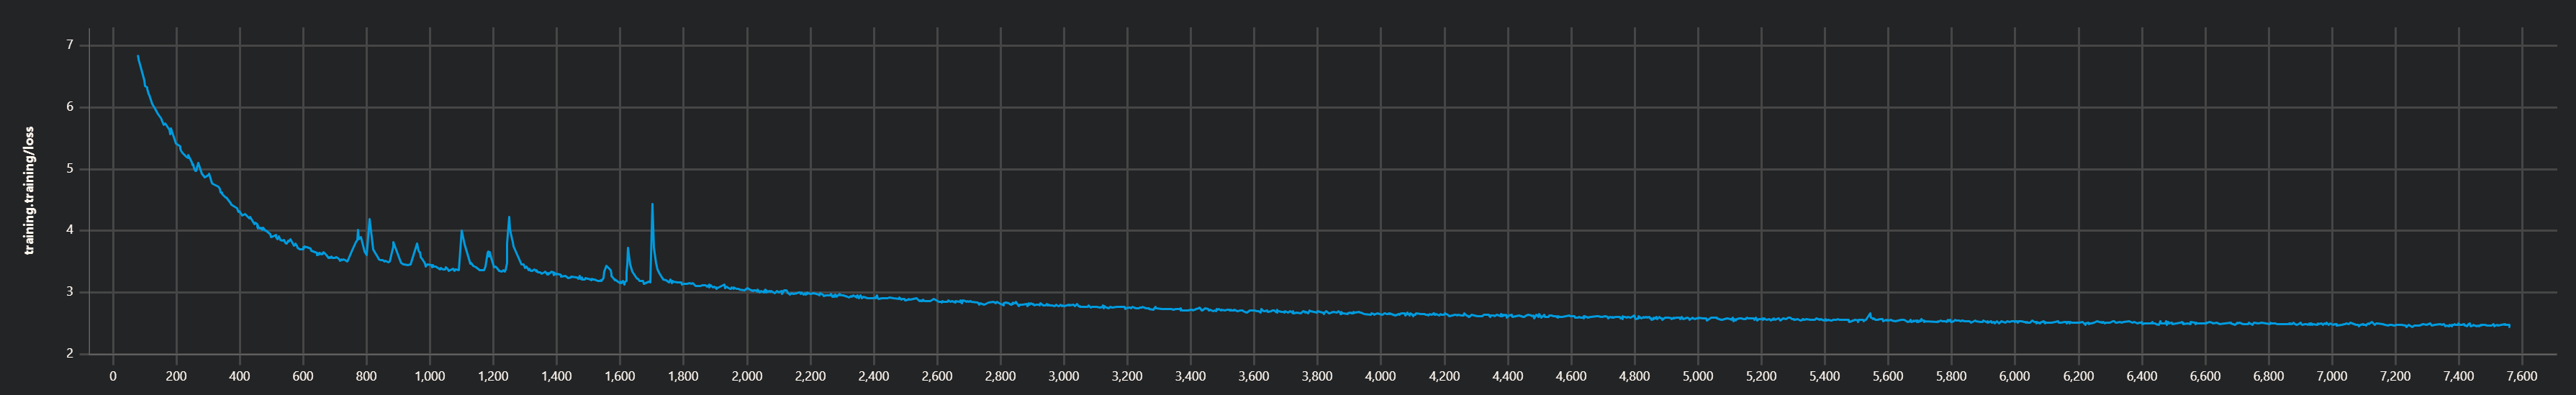
\includegraphics[width=\linewidth]{images/loss_token.png}
    \caption{Classic Tokenizer.}
    \end{subfigure}
    \begin{subfigure}{\linewidth}
    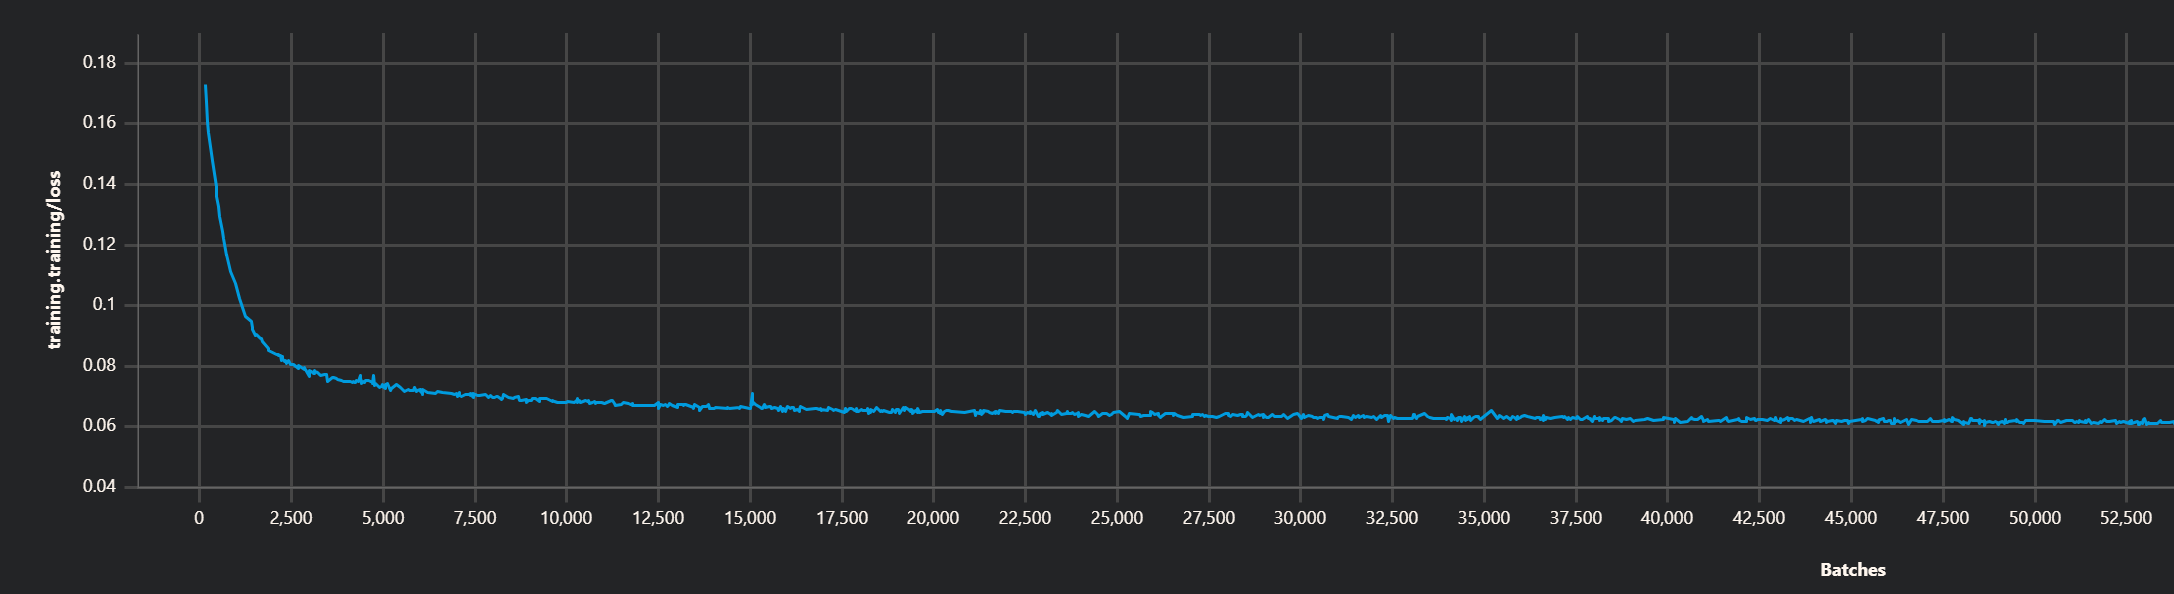
\includegraphics[width=\linewidth]{images/loss_trigram.png}
    \caption{\method.}
    \end{subfigure}
    \caption{Exemplary comparison of classic tokenizer ($v=64k$) training  loss curve (top) and \method\ ($v=16k$) training loss (bottom). Overall we noticed less spikey training behavior when using \method. Both 3B models were trained on same slimpajama data, token-batchsize and learning rate 4.5e-4.}
    \label{fig:training_loss}
\end{figure*}

\begin{figure}
    \centering
    \begin{subfigure}{\linewidth}
    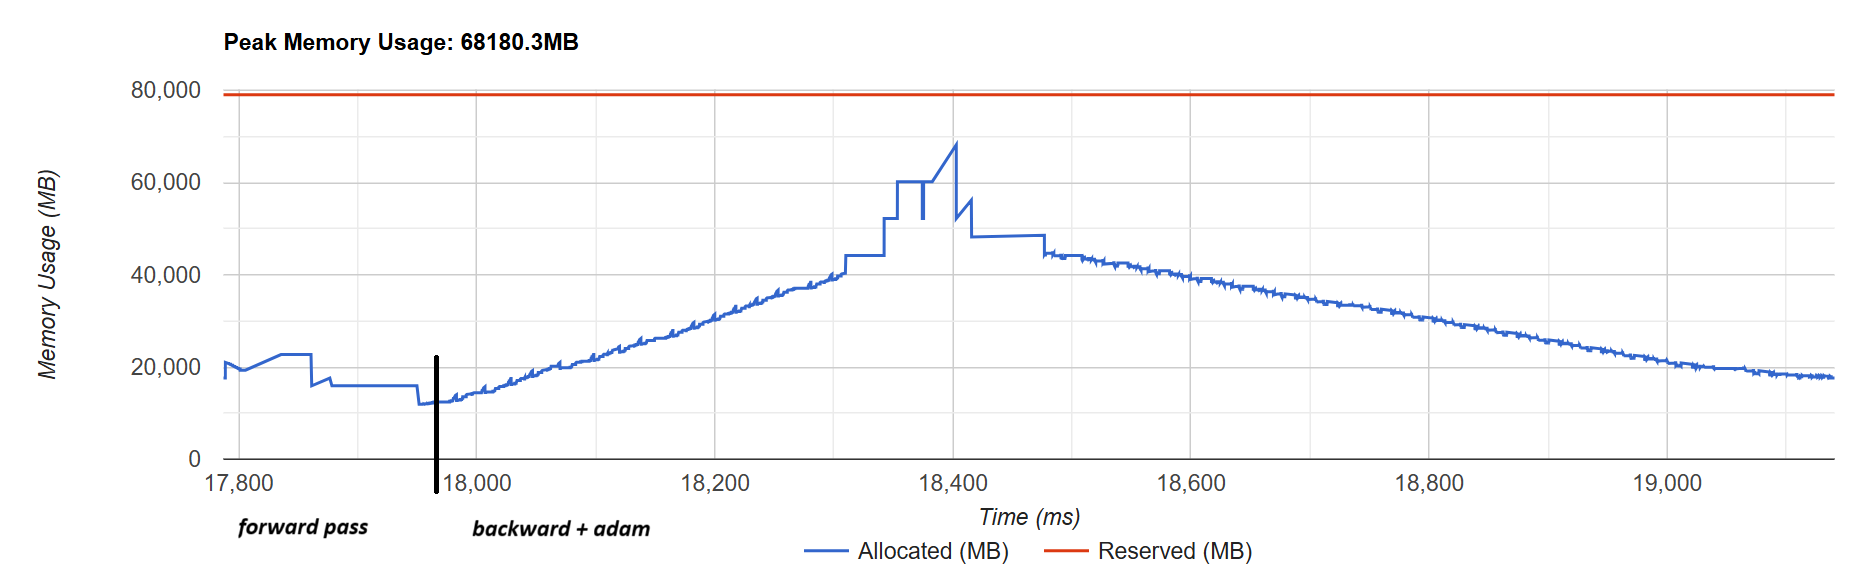
\includegraphics[width=\linewidth]{images/mem_token.png}
    \caption{Classic Tokenizer.}
    \end{subfigure}
    \begin{subfigure}{\linewidth}
    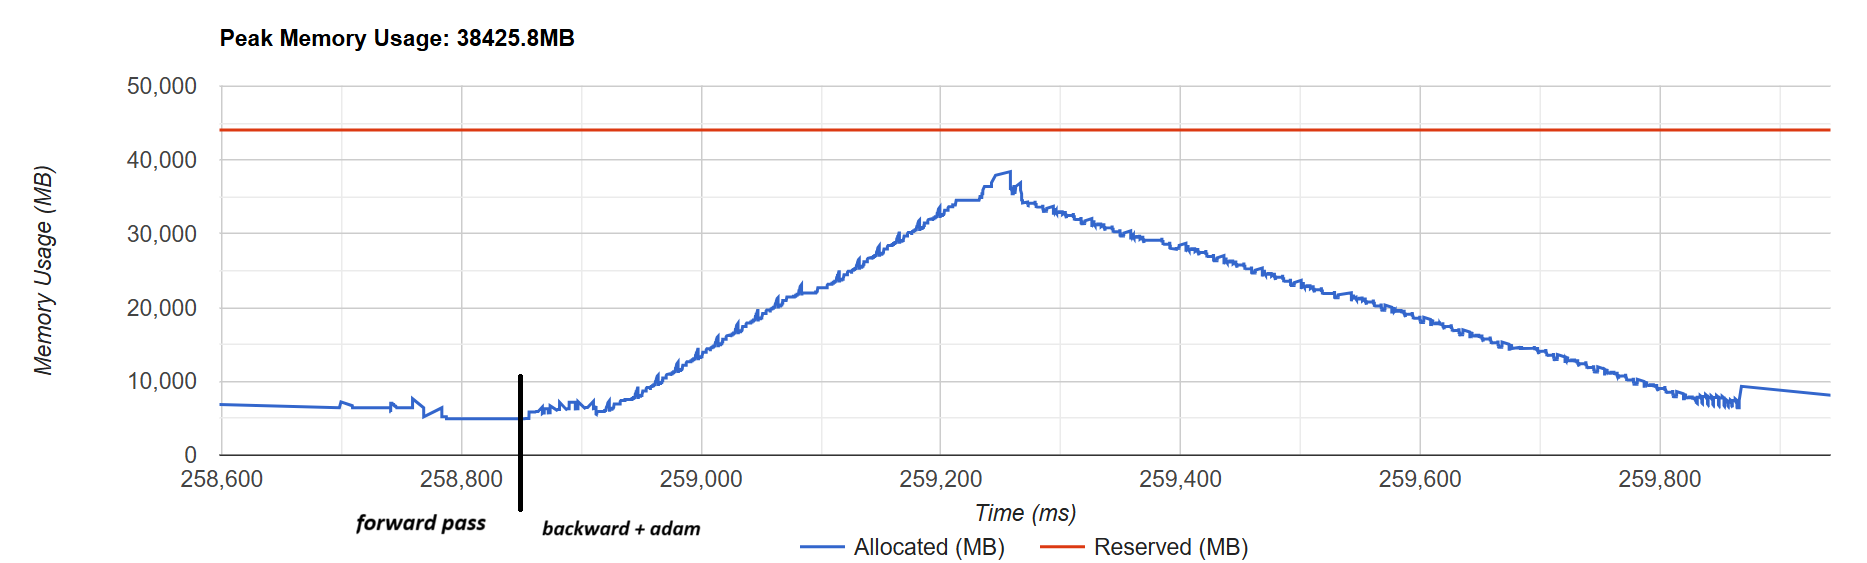
\includegraphics[width=\linewidth]{images/mem_trigram.png}
    \caption{\method.}
    \end{subfigure}
    \caption{Pytorch Profiler Memory Footprint of a single forward and backward pass on a $1B$, each with batch size $8$ and $4k$ sequence length. Top is classical tokenizer version with $64k$ vocab size, bottom trigram with $8k$ vocabulary. Note how AdamW aggregates peak memory consumption until 68GB for classic tokenizer, while ours remains at 38GB.}
    \label{fig:memory_footprint}
\end{figure}


\section{Hyperparameter Ablations}
\emph{Some 1,500 determined experiments later...}

\label{app:hyperparameter_ablation}
Albeit pretty scarse, some more hyper-parameter ablations are found in Fig.~\ref{fig:hyperparameter_hs},\ref{fig:hyperparameter_ablation}.

We will continue to polish and add more...
\begin{figure}
    \centering    
         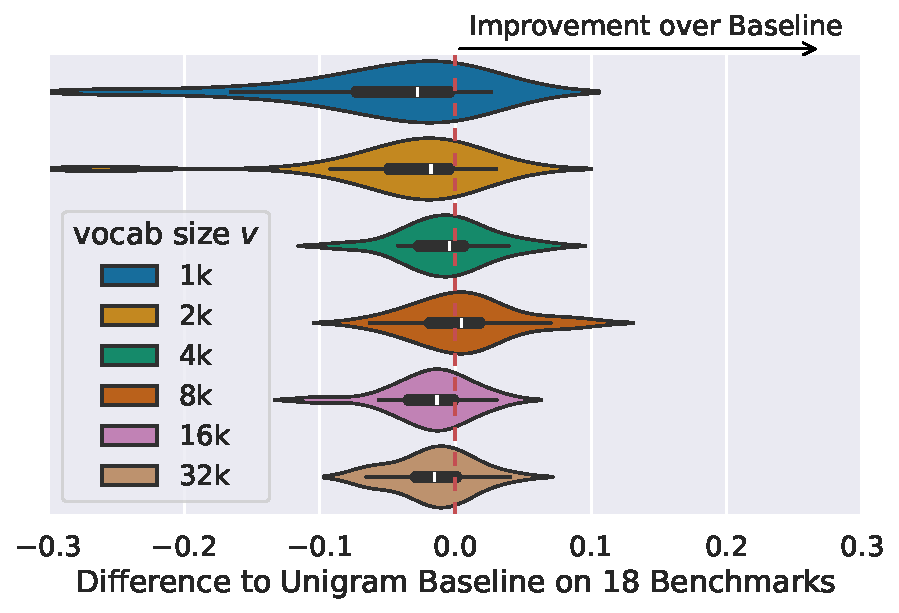
\includegraphics[width=.95\linewidth]{images/ablation_hidden_size.pdf}
         \caption{Further ablations on hyper paramters in accordance to Fig.~\ref{fig:hyperparameter_1b}. Note that after peaking at $v=8k$, performance slightly decreases again, which may be attributed to the undertrained stage of the model trainings.}
    \label{fig:hyperparameter_hs}
\end{figure}

\begin{figure}
    \centering    
         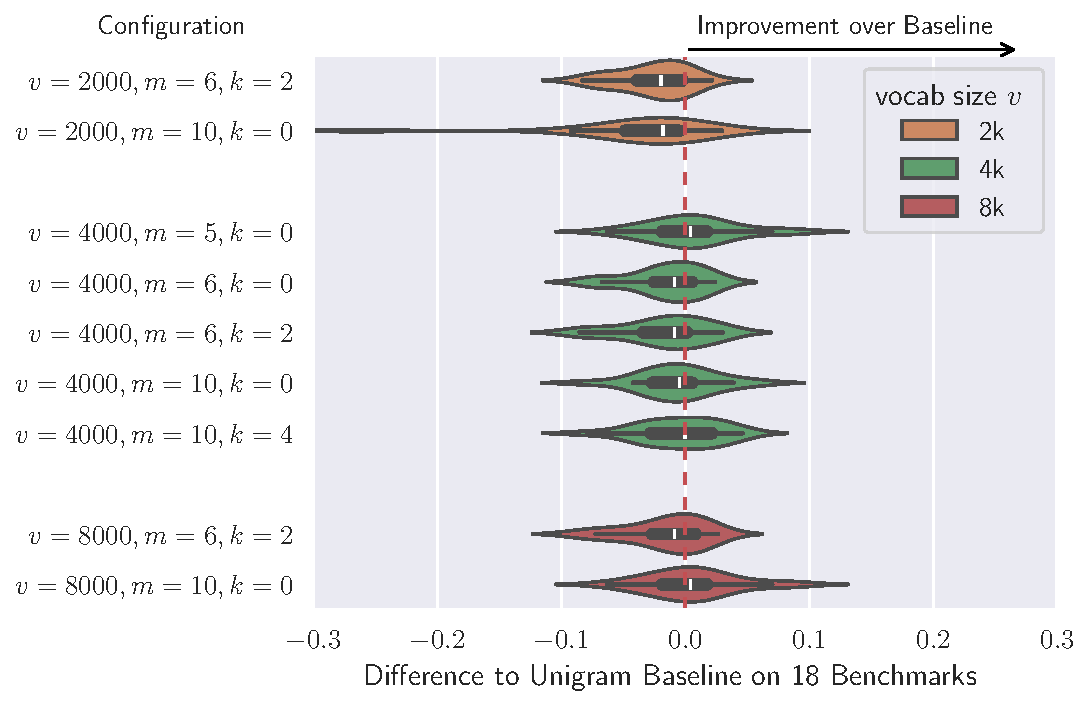
\includegraphics[width=.95\linewidth]{images/ablation_total.pdf}
         \caption{Further ablations on hyper paramters.}
    \label{fig:hyperparameter_ablation}
\end{figure}

\section{Some Statistics}
\label{app:statistics}


\paragraph{Trigram combinatorics.}
As there are more than $v$ possible words, there will naturally be some overlap in the activations between words. However, assuming an embedding dimension of $v \approx 8,000$, $m \approx 8$ activations per trigram, and a word of length $n = 5$, there are (in theory) ${v \choose n \cdot m} \approx 10^{108}$ unique activation patterns. 

This overlap can be interpreted as an interpolation between input states. For entirely independent inputs, this overlap should be kept small as the results cannot benefit from the states of the shared activations.
As such, we require a \emph{robust hash function} on text, i.e. a mapping from text into sparse activation patterns, for which the overlapping of activations is proportional to the similarity of the input words.
We model this through trigrams, and as such, letter-similarity.





\paragraph{Tokenizer Duplicates.}
Tab.~\ref{tab:word_prefixes} shows the curse of token-based vocabularies: to produce all 64 upper and whitespace variations of the word ``\_words'', one requires on average 3 tokens per writing.

\paragraph{Dataset-Coverages.}
Fig.~\ref{fig:top-nwords} shows the covered percentages of the entire dataset, by word-lengths, for all slimpajama datasets.
If we successfully can encode all words of length $\leq 10$, we can cover $\geq 95\%$ of the entire slimpajama dataset. Or conversely, we would only require 5\% outlier handling/ additional splits for longer words (\emph{cf.} Sec.~\ref{sec:conclusion}).

Fig.~\ref{fig:top_100k} and Fig.~\ref{fig:trigrams} show dataset coverage (y-axis) of top-n words and trigrams (x-axis) for each slimpajama category. Notably 10k trigrams, and 100k words consistently cover $>95\%$ of each slimpajama category.


\begin{table}[]
    \centering
    \begin{tabular}{c c}
    string & token id \\
    \hline\hline
`\_' & 49594 \\
\hline
`\_w'& 15997 \\
`W'& 40669 \\
`\_W'& 46854 \\
`w'& 63048 \\
\hline
`Wo'& 7411 \\
`\_wo'& 14297 \\
`\_WO'& 14883 \\
`wo'& 34034 \\
`\_Wo'& 39790 \\
`WO'& 44468 \\
\hline
`WOR'& 1916 \\
`\_WOR'& 6606 \\
`\_Wor'& 40813 \\
\hline
`\_Word'& 1971 \\
`Word'& 3212 \\
`\_word'& 14272 \\
`WORD'& 48022 \\
`word'& 49922 \\
\hline
`\_words'& 12555 \\
`words'& 28689 \\
`WORDS'& 32751 \\
`\_Words'& 37912 \\
`Words'& 51858\\
    \end{tabular}
    \caption{The 24 possible first tokens to construct uppercase and whitespace variations of ``\_words'', where ``\_'' denotes a whitespace. In total, there are 64 ways to write ``\_words'', which requires $32\cdot 6 + 32\cdot 5=342$ characters. 
    The tokenizer requires in total 194 tokens, of which 37 are unique, leading to an average (neglecting the occurrence frequencies) of $\approx3$ tokens per writing.}
    \label{tab:word_prefixes}
\end{table}




\begin{figure*}
    \centering
    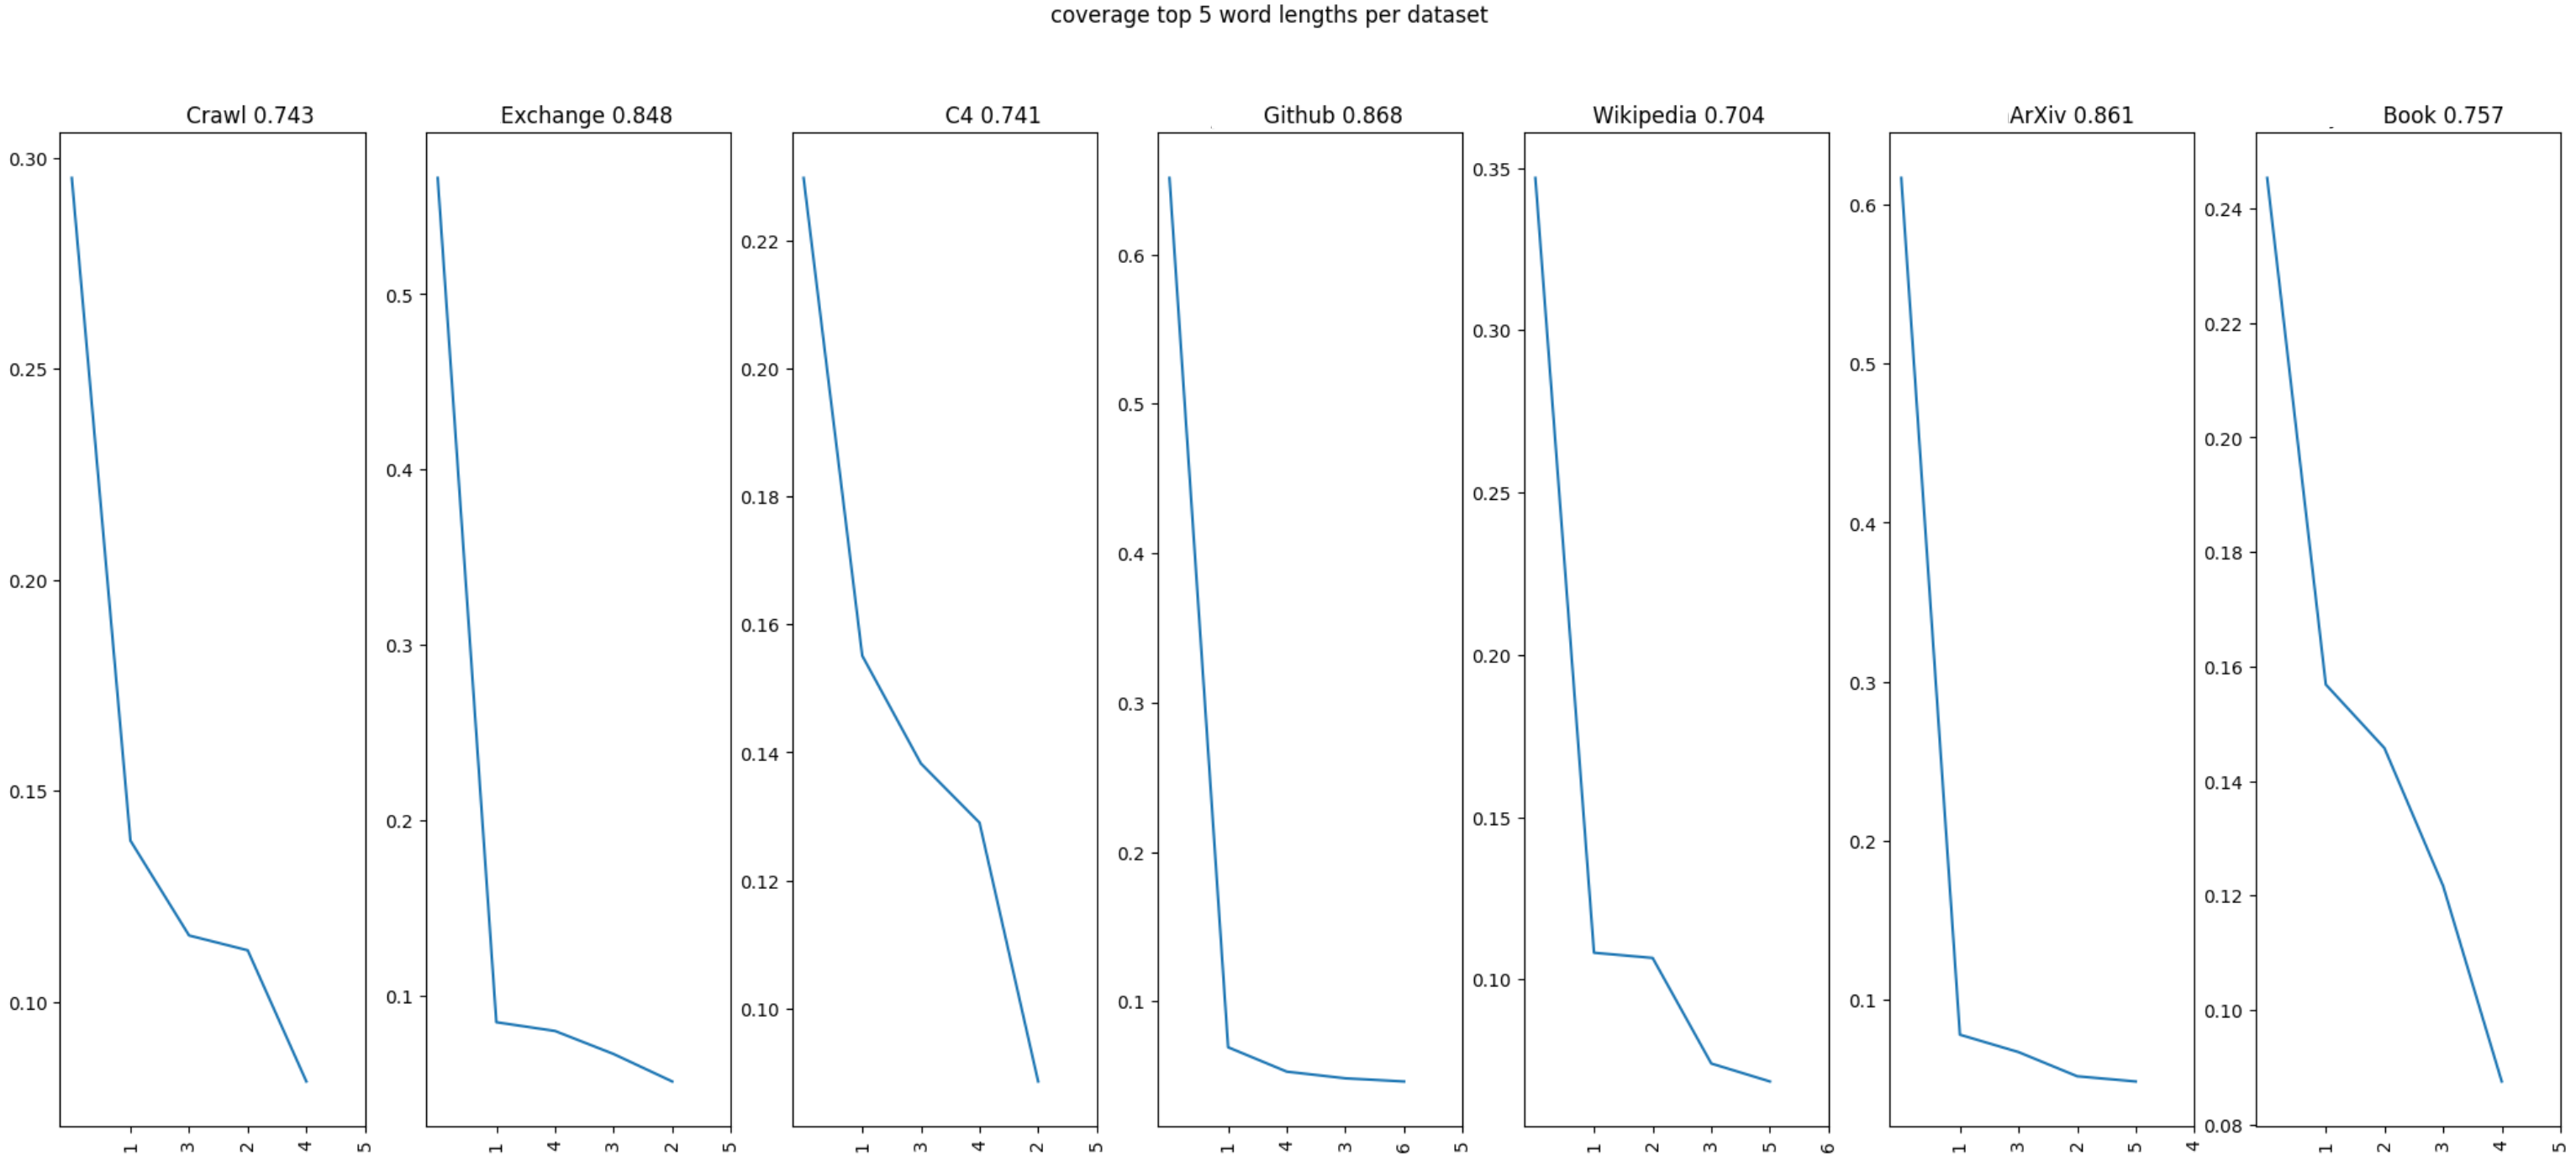
\includegraphics[width=\linewidth]{images/draft/top5_wordlength.png}
    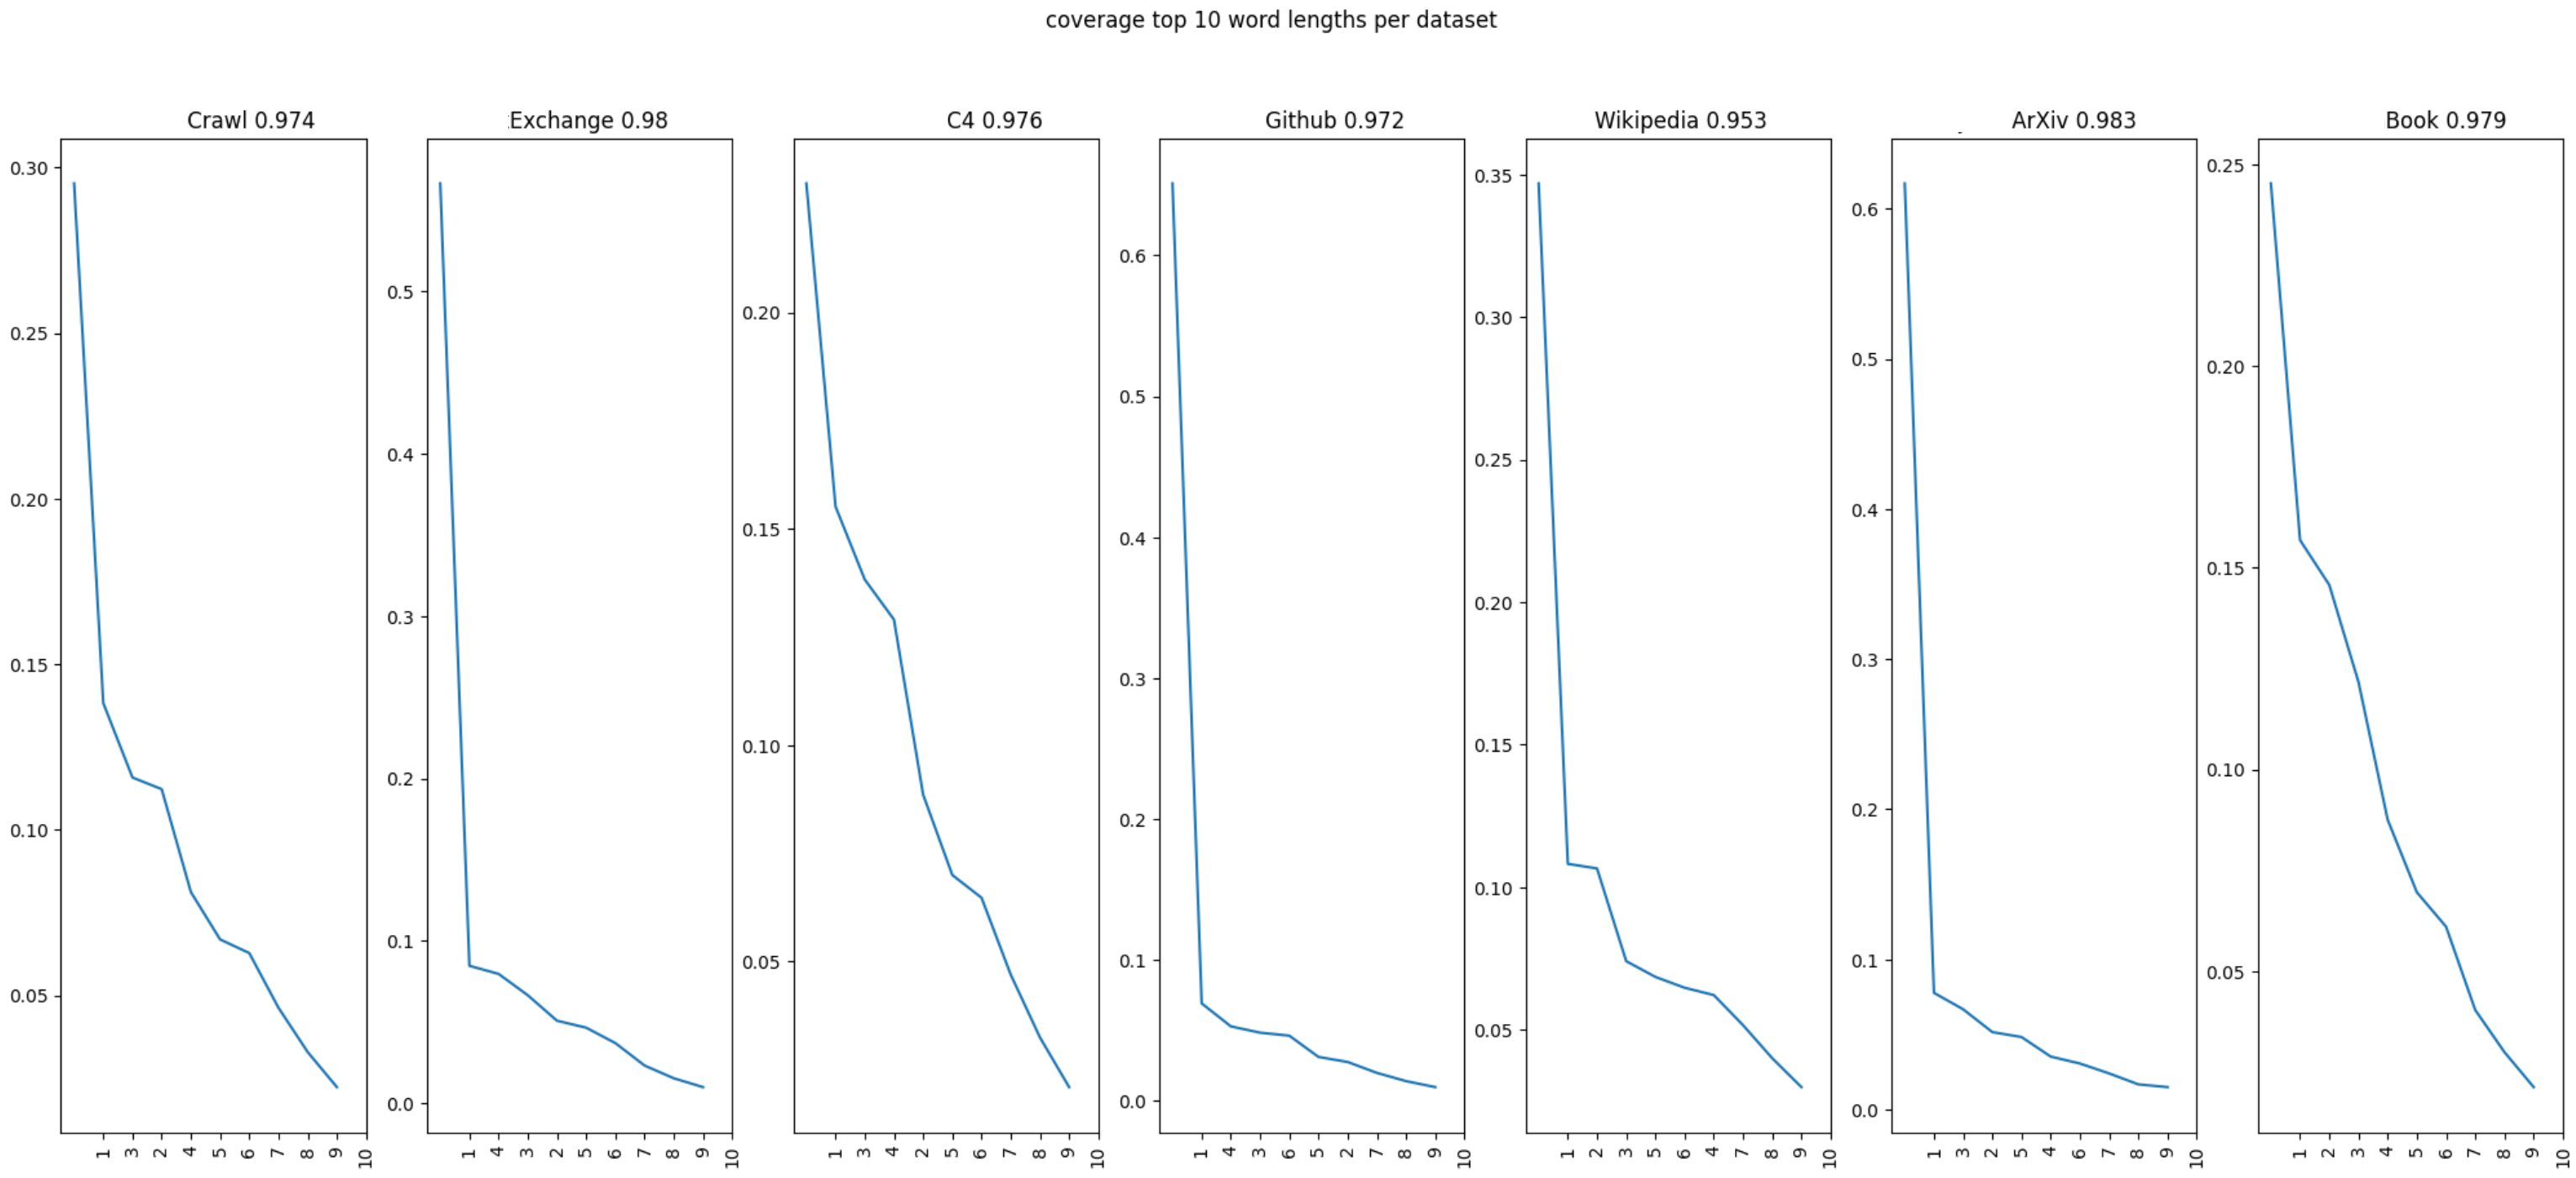
\includegraphics[width=\linewidth]{images/draft/top10_wordlength.png}
    \caption{Top 5 and top 10 occuring word lengths (x-axis) per slimpajama data category, with coverage-percentage (y-axis).  Headline indicates total percentage covered by top $n$-length words. With words of length $\leq 5$, one always covers $\geq 74\%$ of all occuring words. With all words of length $\leq 10$, one achieves $\geq 95\%$.}
    \label{fig:top-nwords}
\end{figure*}

% \begin{table}\centering
% \begin{tabular}{c|c}
%    \# words  & coverage (\%) \\
%    \hline
%     10 & 25.2\\
%     100 & 52.1 \\
%     1,000 & 70.2 \\
%     10,000 & 89.4\\
%     100,000 & 98.0\\
%     1,000,000 & 99.7\\
% \end{tabular}
\begin{figure*}
    \centering
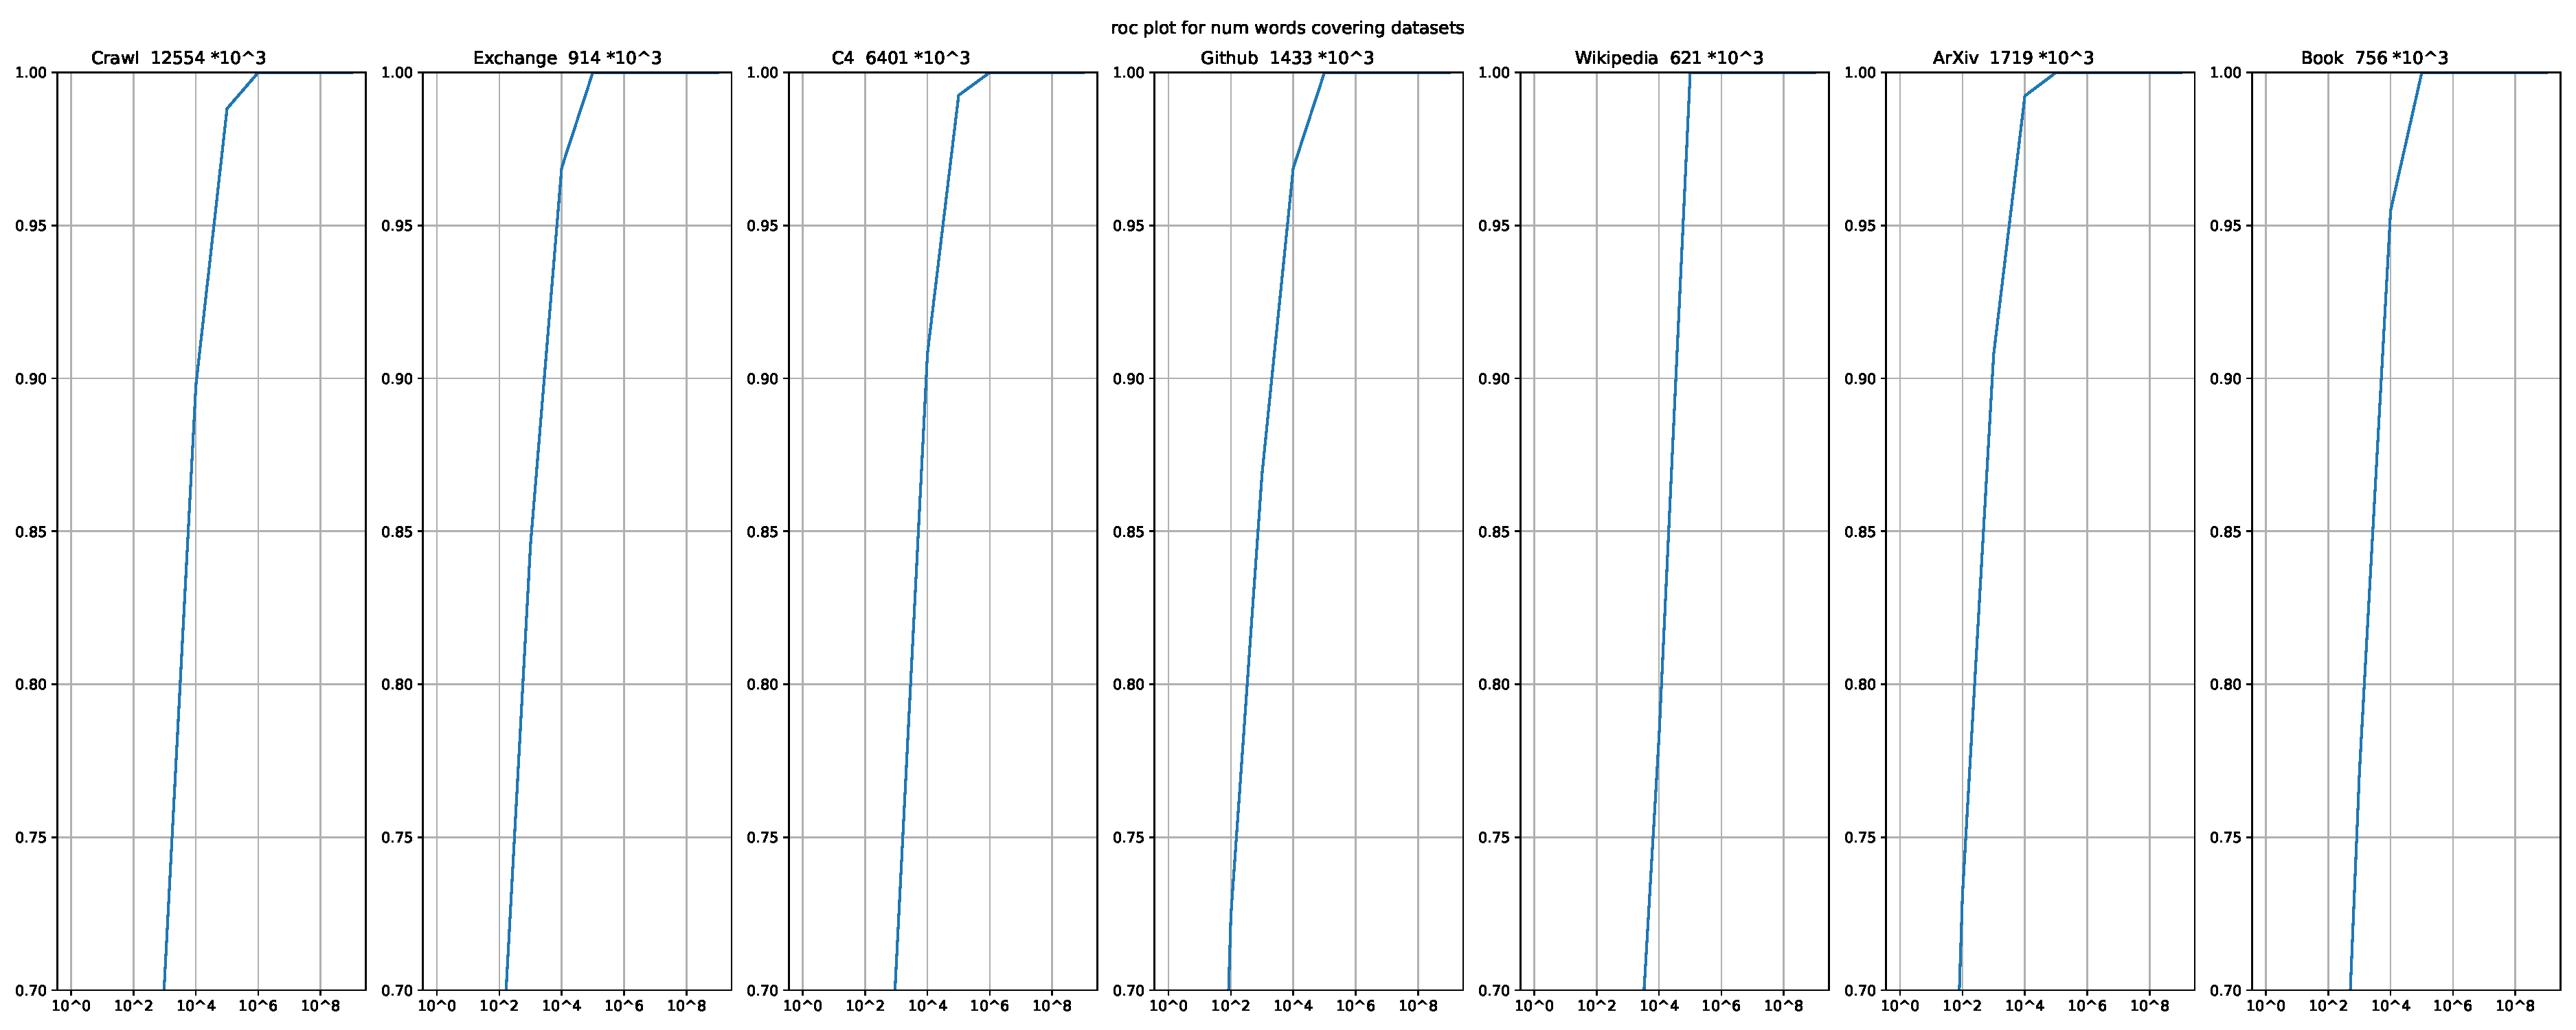
\includegraphics[width=\linewidth]{images/total_words.pdf}
\caption{Most-frequent word coverage of Slimpajama categories.  Title shows the total number of words per dataset sample, $x$-axis the top-n chosen words, $y$-axis the percentage covered within dataset. With only 100k words we can consistenly cover $> 95\%$ of each category.}
\label{fig:top_100k}
\end{figure*}

\begin{figure*}
    \centering
    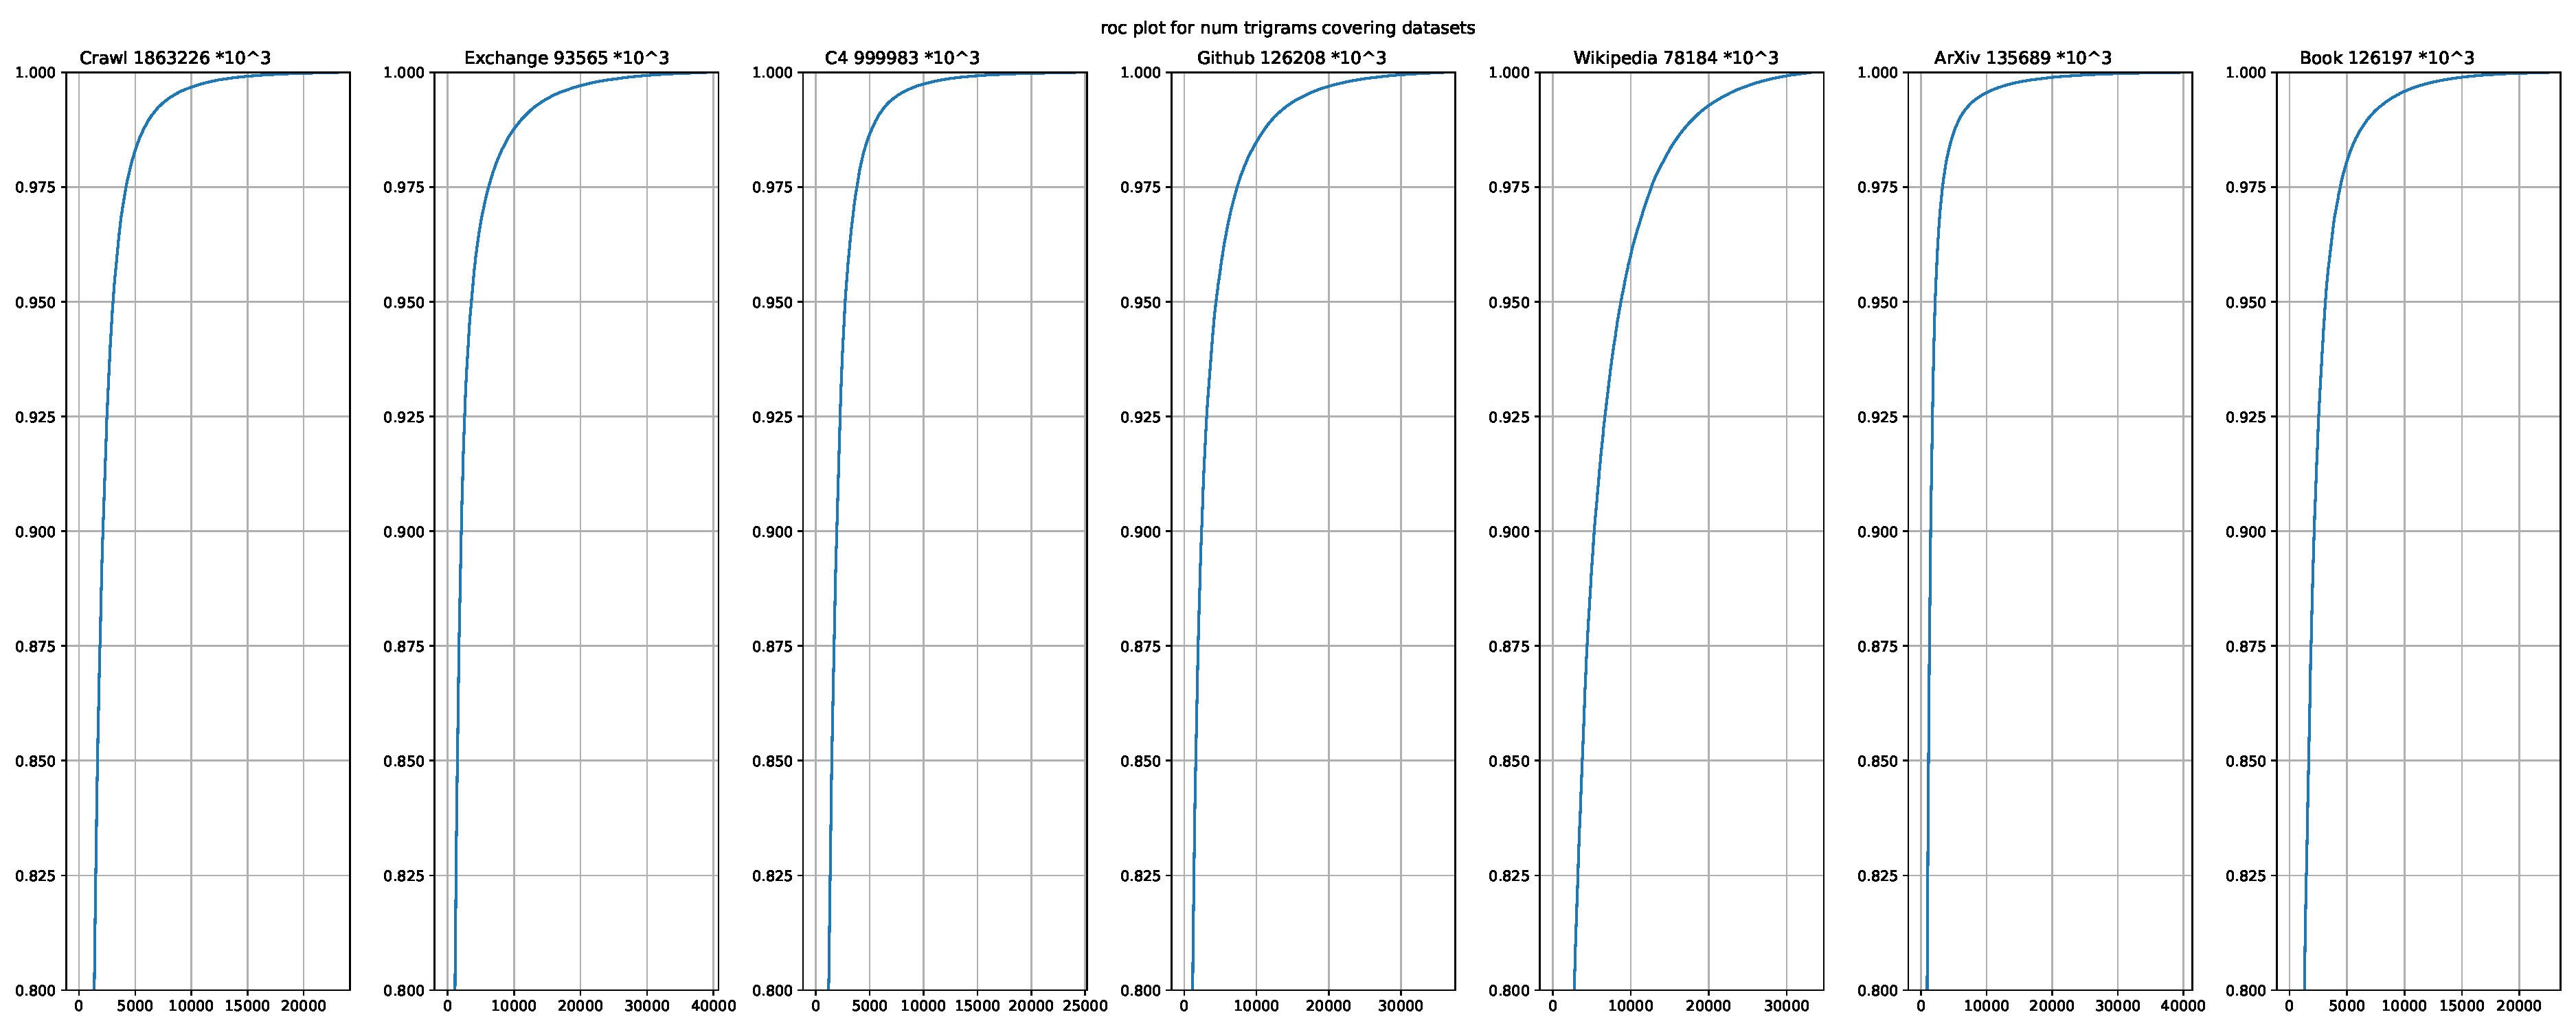
\includegraphics[width=\linewidth]{images/total_trigrams.pdf}
    \caption{Number of trigrams ($x$-axis) required to cover ($y$-axis) percentage of the categories of slimpajama (total number words sampled in title). With only 10k trigrams we can cover $> 95\%$ of all occuring words.}
    \label{fig:trigrams}
\end{figure*}



\section{More Benchmarks}
\label{app:benchmarks}
We used the code of the eleuther eval harness, and evaluated each benchmark in 0-shot and 2-shot. All 18 benchmarks, namely
\textit{arc (easy and challenge), hellaswag, winogrande, triviaqa, xnli, truthfulqa, boolq, copa, openbook, piqa, multirc, lambada (openai and standard), race, rte, wic, webqs}
are visualized in Fig.~\ref{fig:plot_all1} and
Fig.~\ref{fig:plot_all2} for a baseline model trained on english slimpajama only and continued finetuning on german occiglot. 
Arc-challenge, hellaswag, xnli and truthfulqa are also evaluated in german translations.
Detailed numbers can be found in Tab.~\ref{tab:evalende},\ref{tab:evalen1} and \ref{tab:evalen2}.


\begin{figure*}
    \centering
    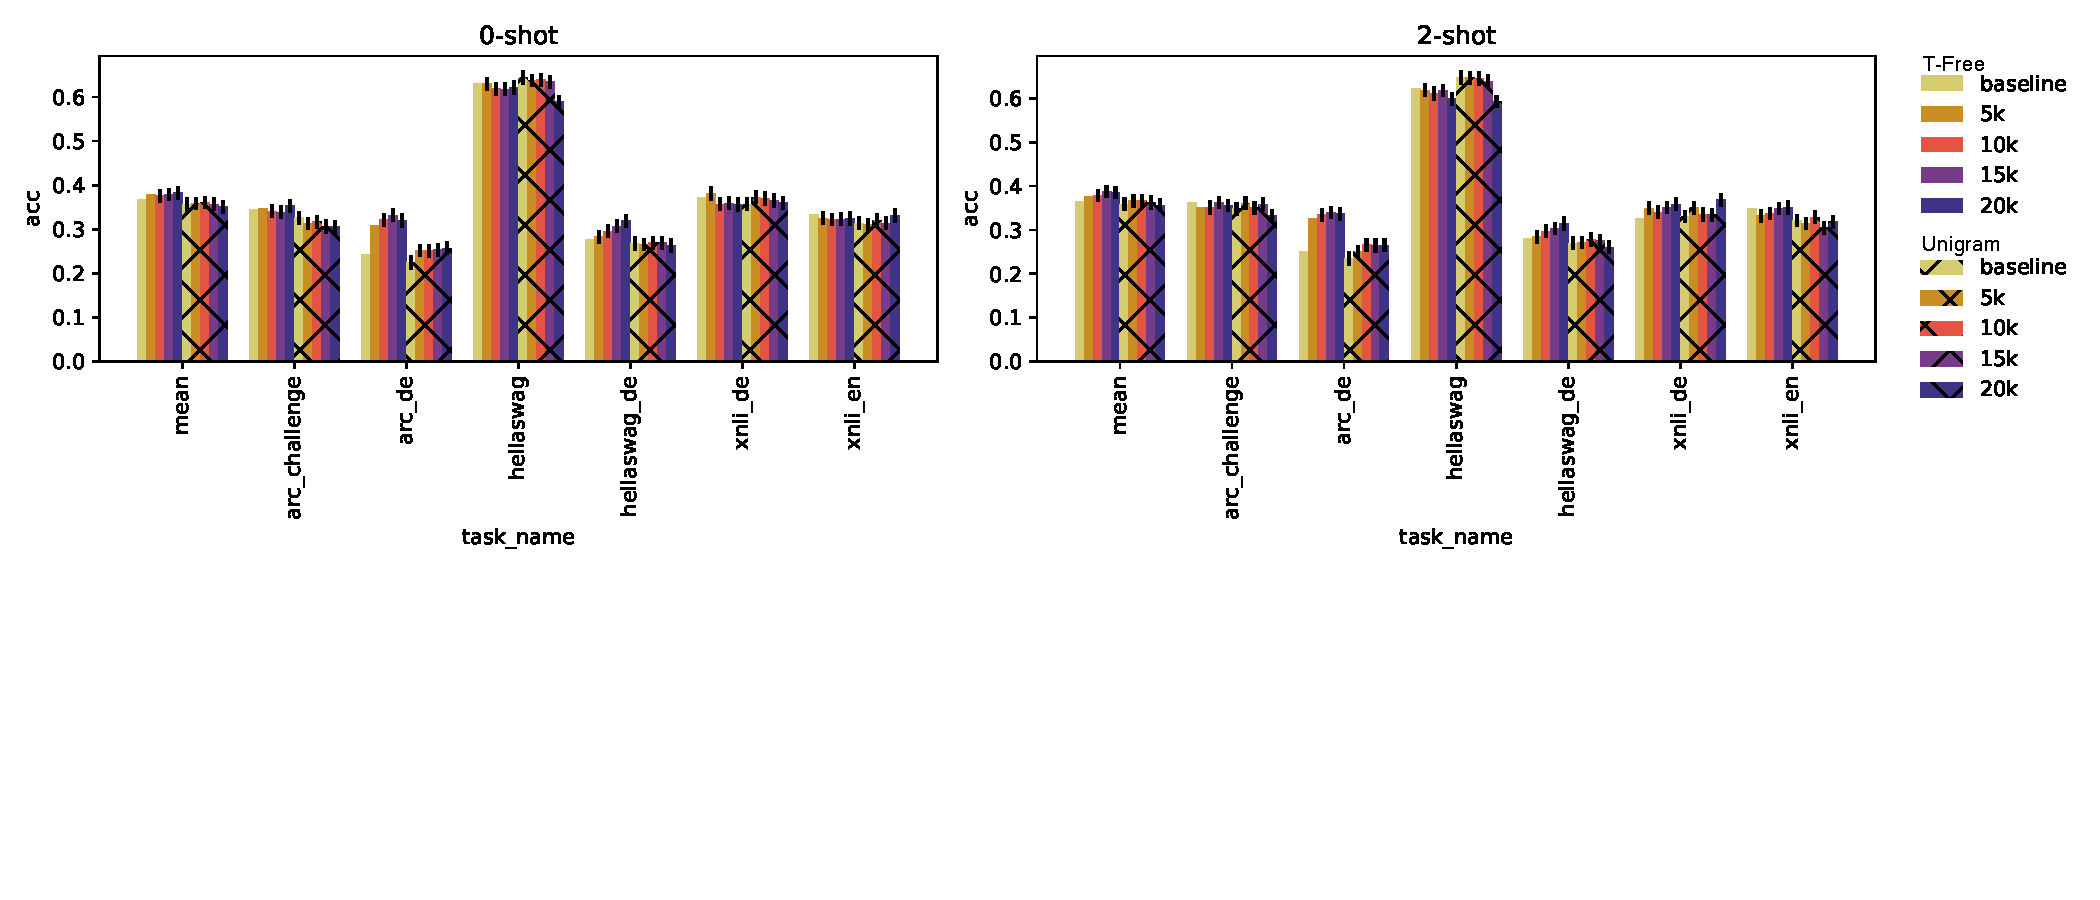
\includegraphics[width=\linewidth,clip,trim=0 5cm 0 0]{images/plot_de_en.pdf}
    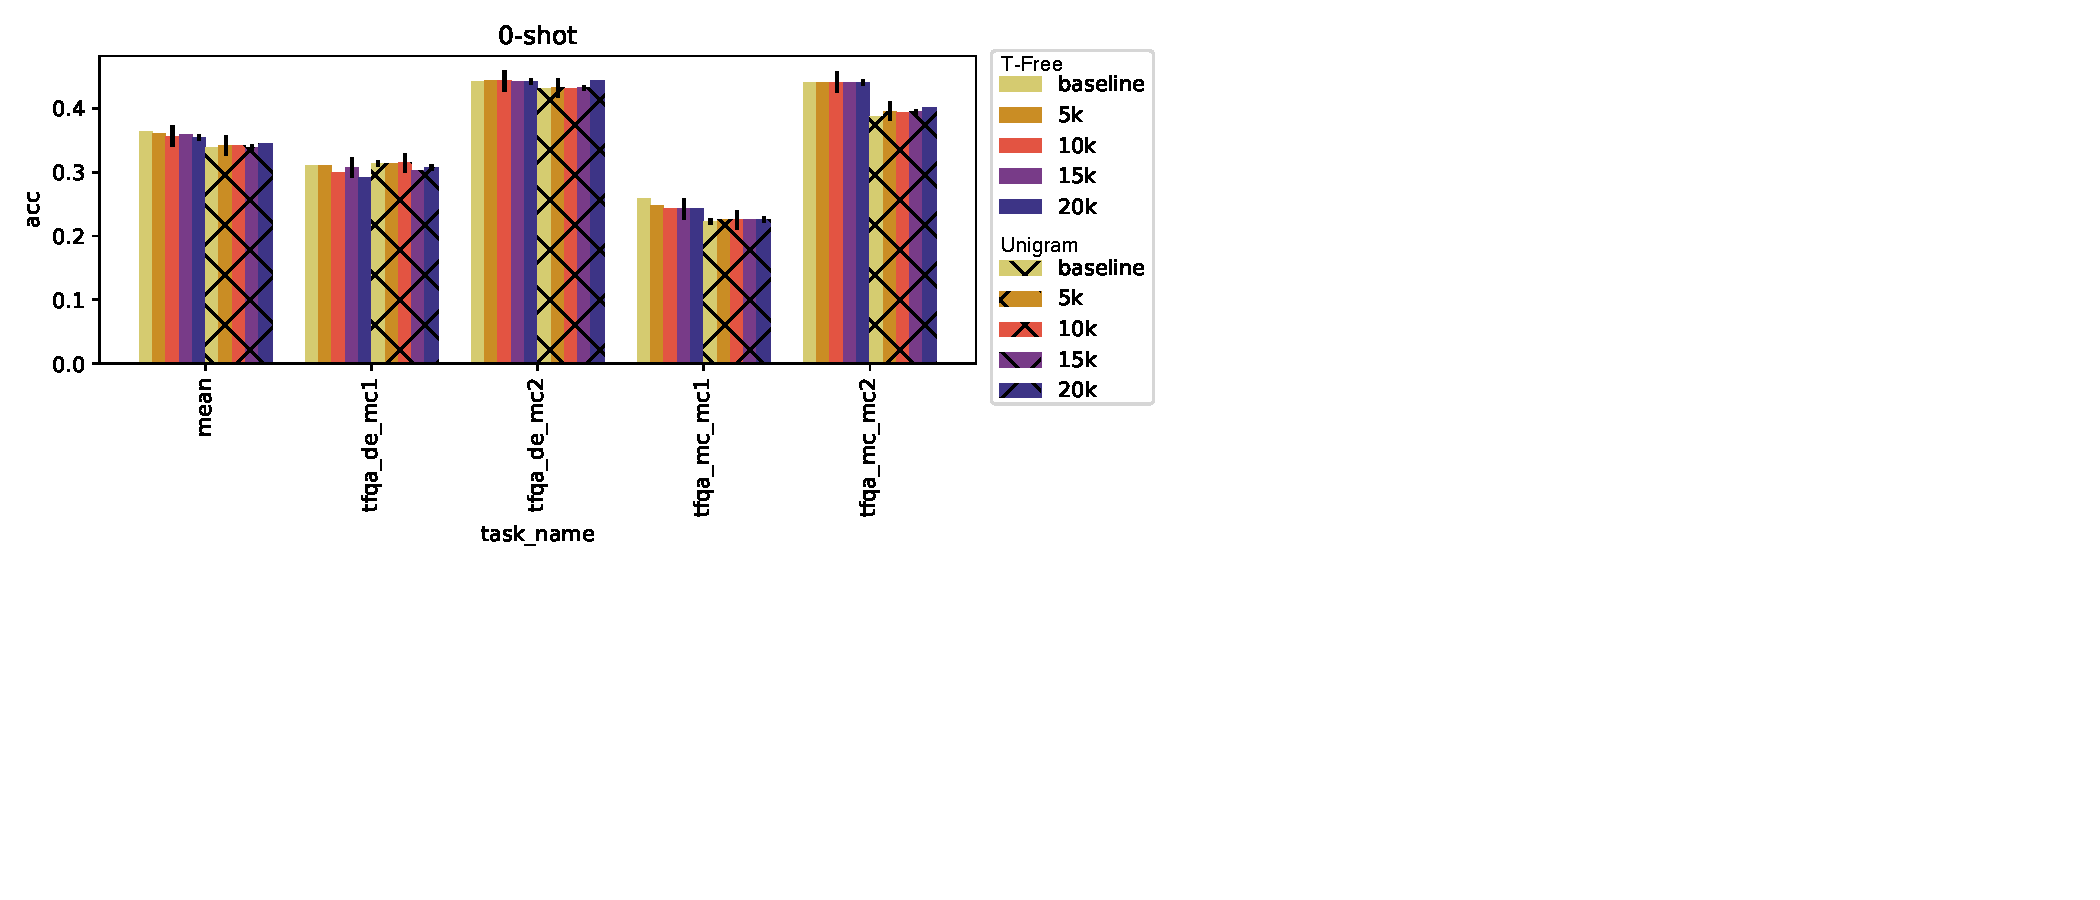
\includegraphics[width=\linewidth,clip,trim=0 5cm 0 0]{images/plot_truthful.pdf}
    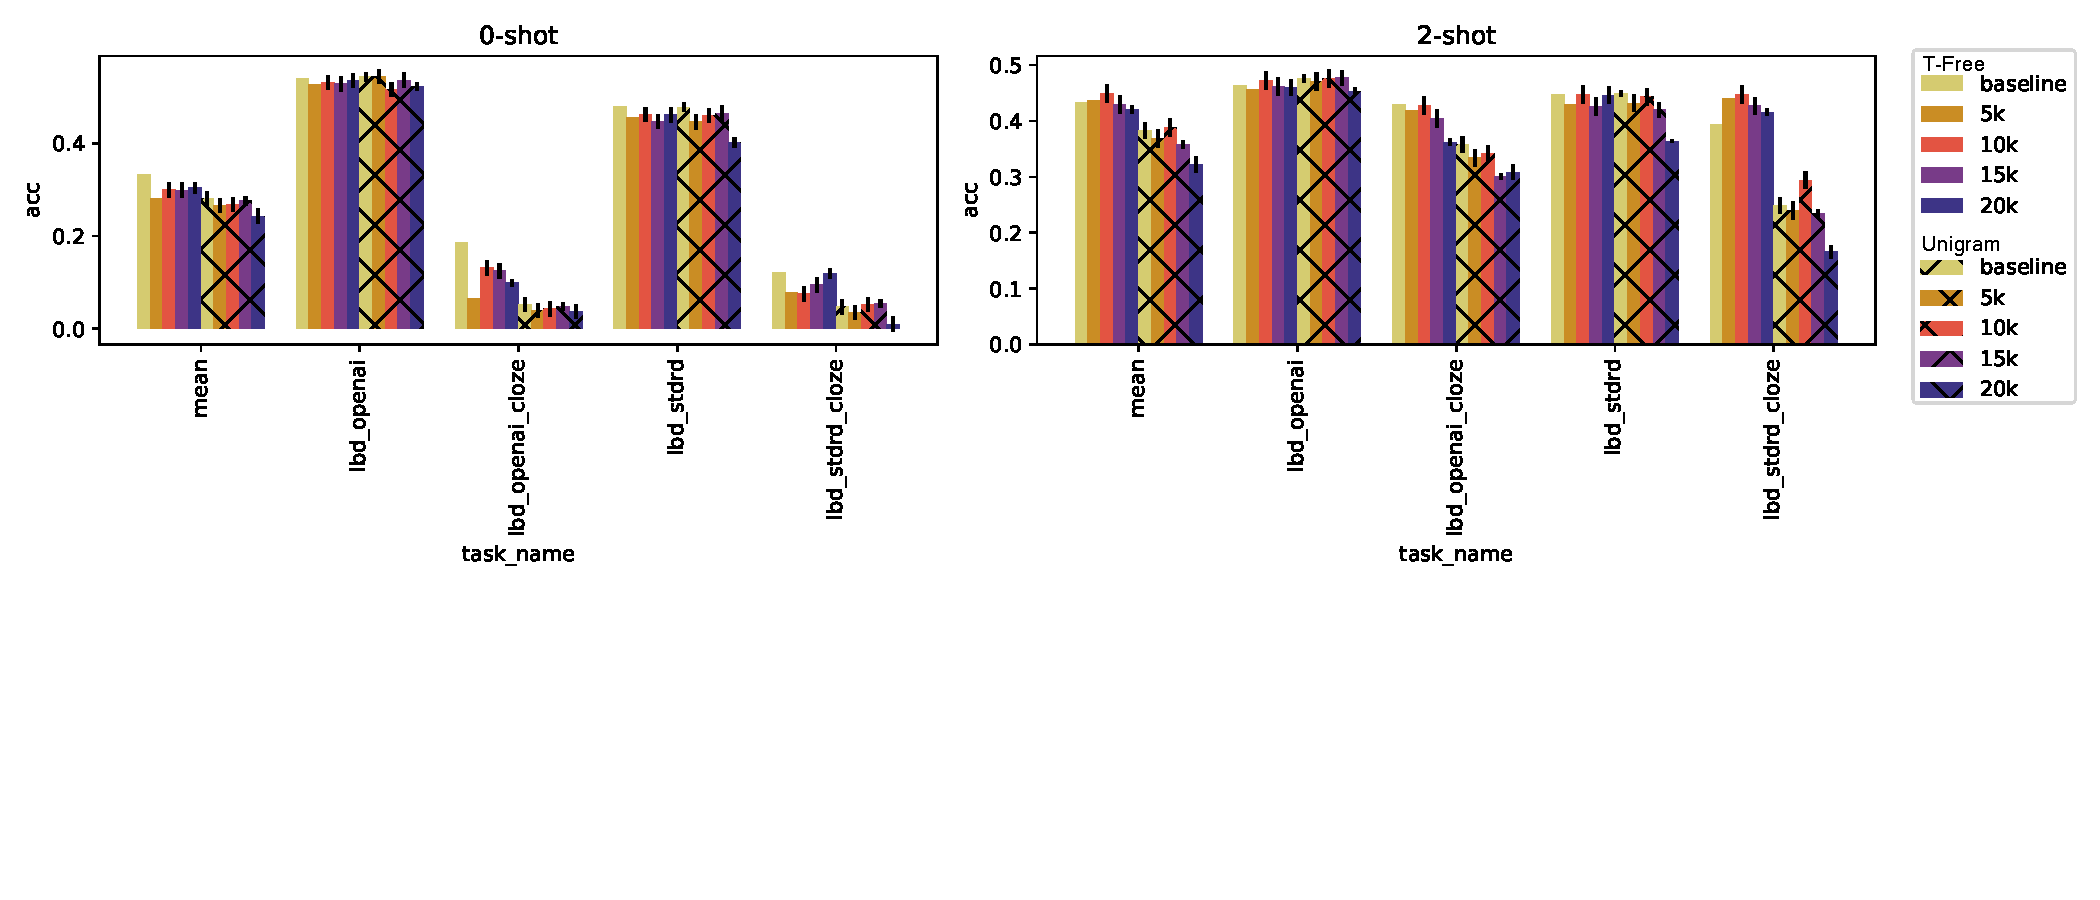
\includegraphics[width=\linewidth,clip,trim=0 5cm 0 0]{images/plot_lambada.pdf}
    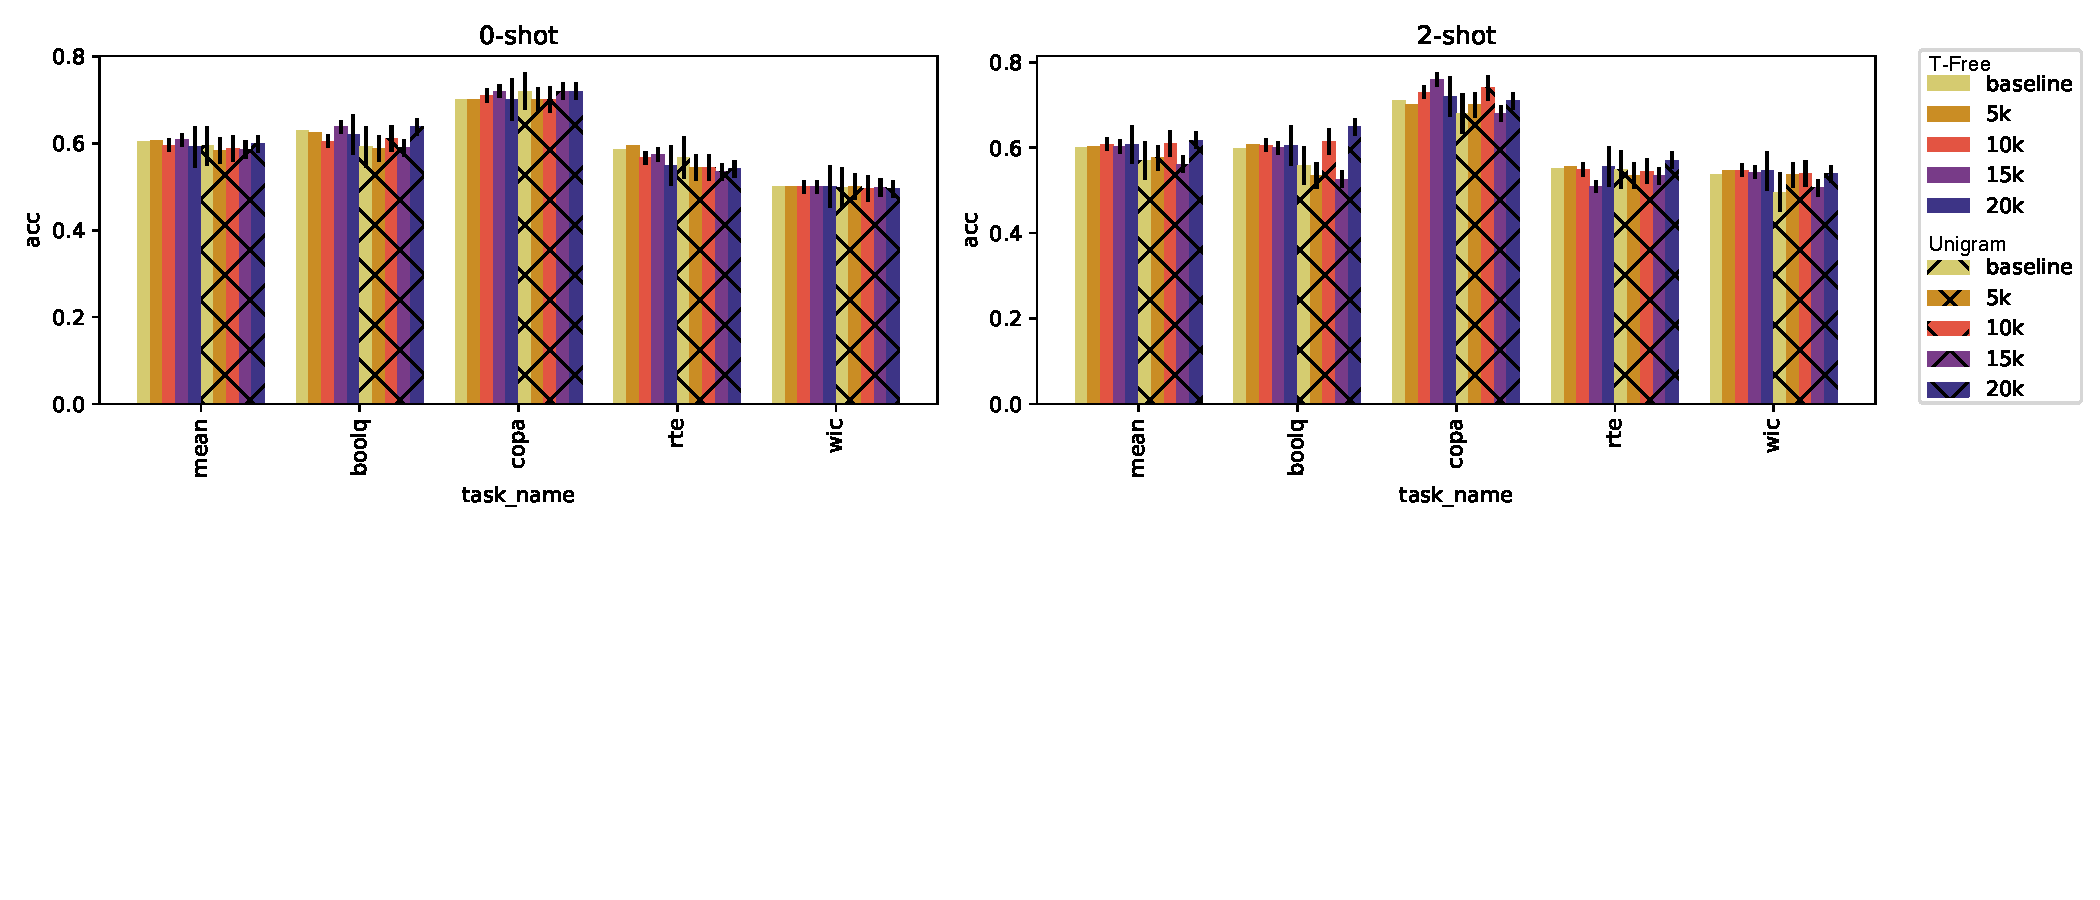
\includegraphics[width=\linewidth,clip,trim=0 5cm 0 0]{images/plot_bools.pdf}    
    \caption{Detailed benchmark results on evaluations of Sec.~\ref{sec:main_results}.}
    \label{fig:plot_all1}
\end{figure*}
\begin{figure*}
    \centering
    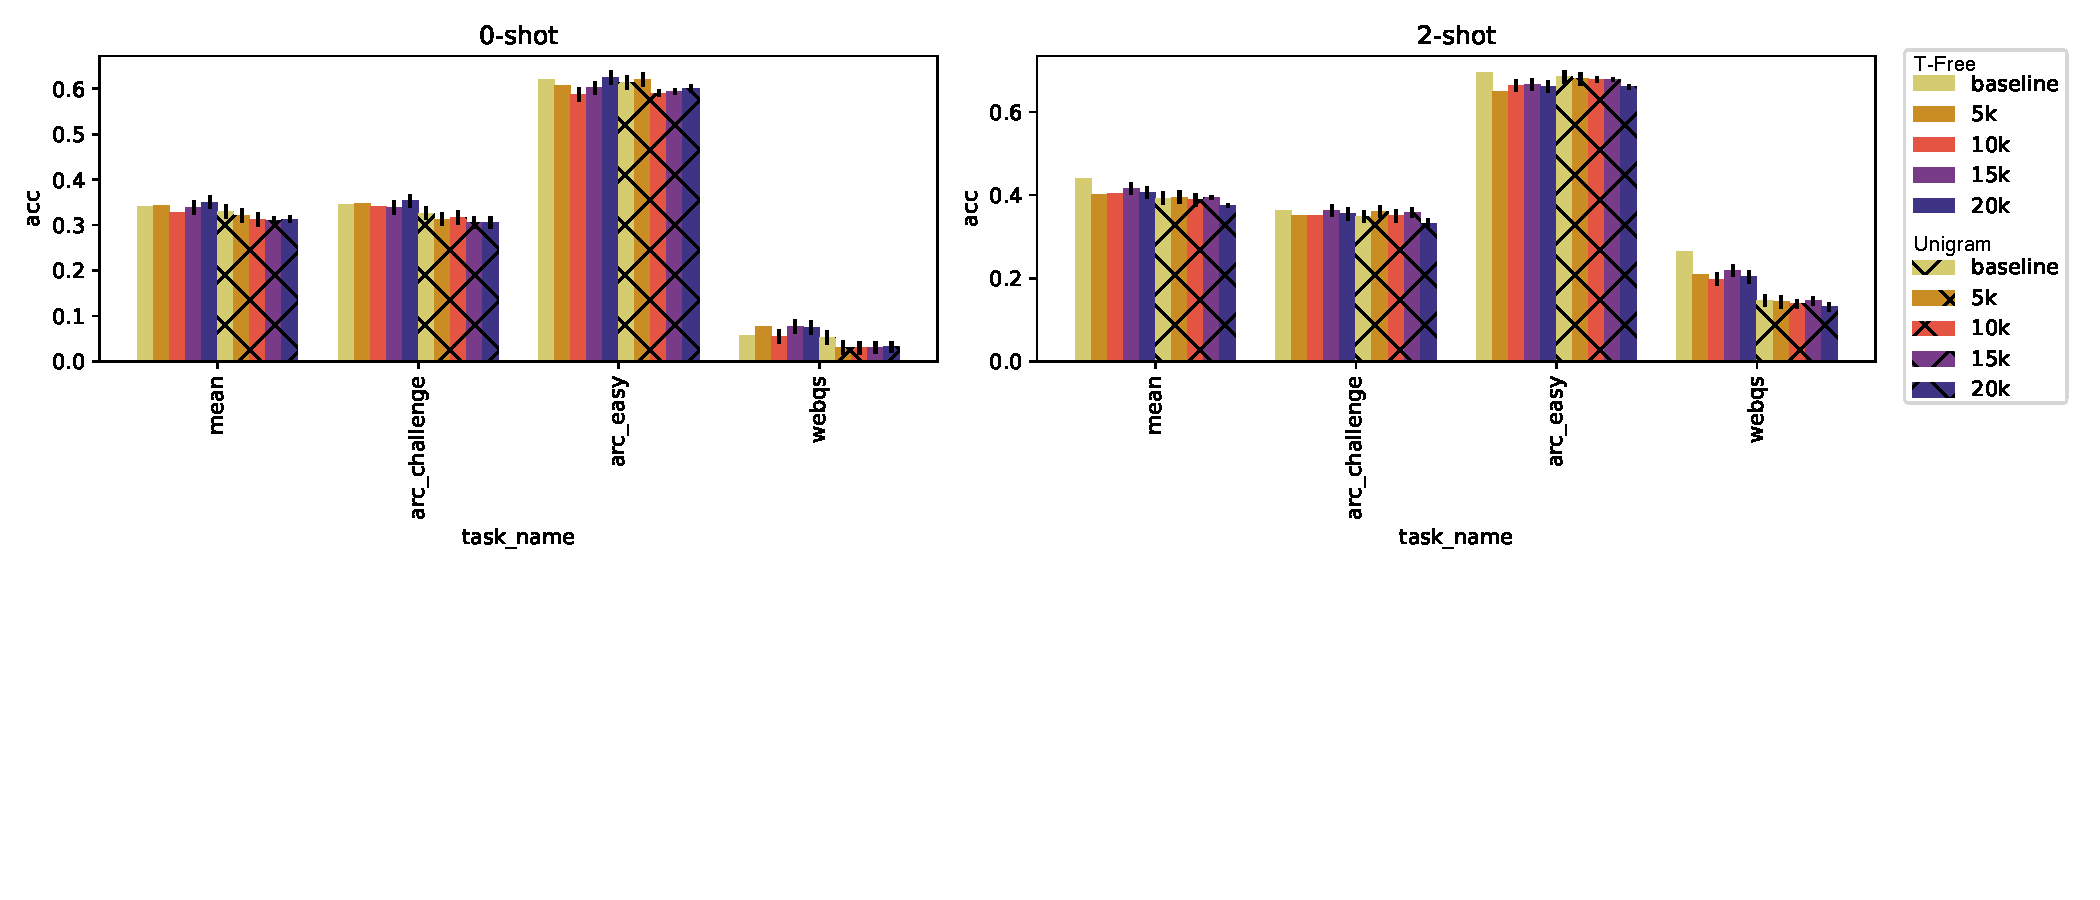
\includegraphics[width=\linewidth,clip,trim=0 5cm 0 0]{images/plot_logic.pdf}
    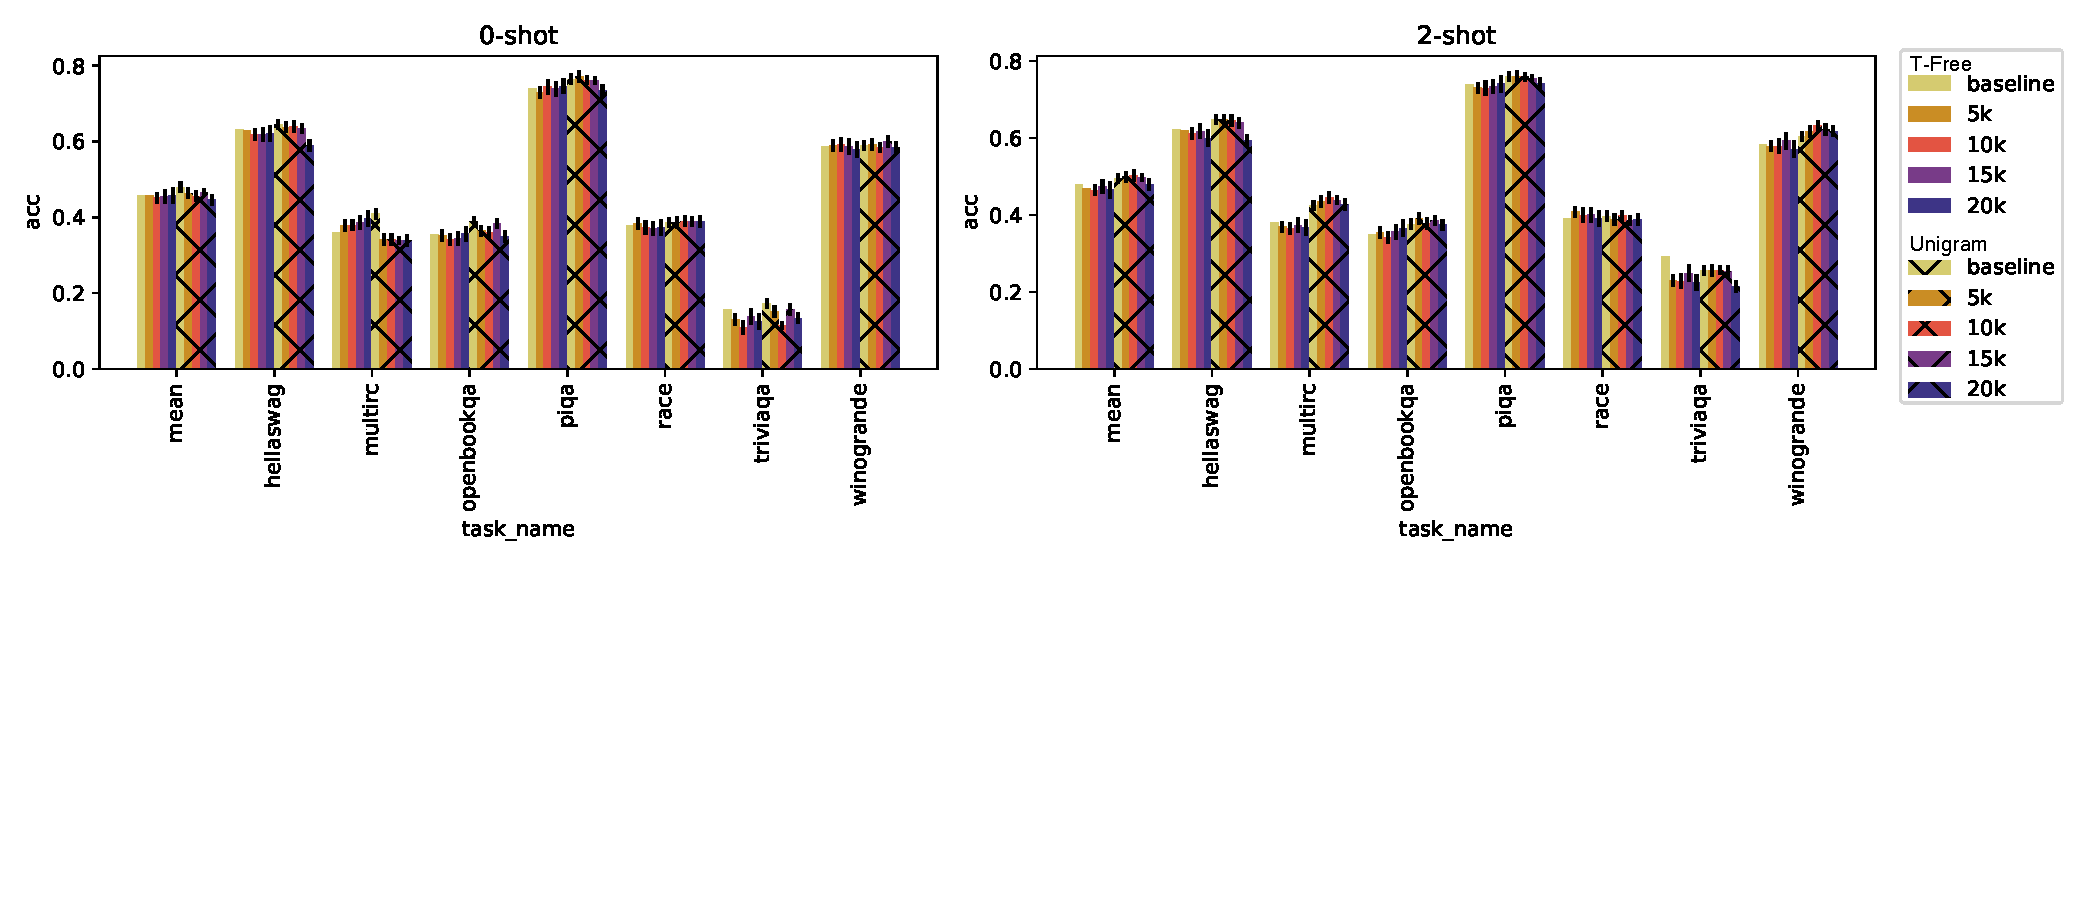
\includegraphics[width=\linewidth,clip,trim=0 5cm 0 0]{images/plot_standard.pdf}
    \caption{Further detailed benchmark results on evaluations of Sec.~\ref{sec:main_results}.}
    \label{fig:plot_all2}
\end{figure*}


\begin{table*}[]
\setlength{\tabcolsep}{5pt}
\small
    \centering
    \begin{tabular}{l l | r r r r r | r r r r r }
    \multicolumn{2}{c}{\multirow{2}{*}{\textbf{Model}}} & \multicolumn{5}{ c |}{\textbf{english benchmarks}} & \multicolumn{5}{ c }{\textbf{german benchmarks}}\\
        &  & $arc_{ch}$ & $hella$ & $xnli$ & $tf_{mc1}$ &  $tf_{mc2}$ &  $arc_{ch}$ & $hella$ & $xnli$ & $tf_{mc1}$ &  $tf_{mc2}$ \\ \hline \hline

        \parbox[t]{1mm}{\multirow{2}{*}{\rotatebox[origin=c]{90}{base}}} & 
  T-Free & 34.5/36.2 & 63.1/62.2 & 33.4/34.8 & 25.9/- & 44.1/- & 24.3/25.0 & 27.7/28.1 & 37.1/32.7 & 31.1/- & 44.3/-\\
 & Unigram & 32.6/34.8 & 64.5/64.8 & 31.4/32.1 & 22.3/- & 38.8/- & 22.5/23.5 & 26.8/27.0 & 35.7/33.1 & 31.3/- & 43.1/-\\
\hline\parbox[t]{1mm}{\multirow{2}{*}{\rotatebox[origin=c]{90}{5k}}} & T-Free & 34.7/35.1 & 63.0/61.9 & 32.5/33.2 & 24.7/- & 44.1/- & 30.9/32.5 & 28.3/28.4 & 38.1/34.9 & 31.1/- & 44.3/-\\
 & Unigram & 31.3/36.1 & 63.8/64.7 & 31.1/31.5 & 22.6/- & 39.6/- & 25.2/25.1 & 26.6/27.2 & 37.3/35.0 & 31.3/- & 43.2/-\\
\hline\parbox[t]{1mm}{\multirow{2}{*}{\rotatebox[origin=c]{90}{10k}}} & T-Free & 34.1/35.1 & 61.9/61.1 & 32.2/33.8 & 24.2/- & 44.1/- & 32.1/33.4 & 29.6/29.7 & 35.7/34.0 & 30.0/- & 44.3/-\\
 & Unigram & 31.7/35.0 & 63.9/64.5 & 32.0/32.9 & 22.5/- & 39.4/- & 25.1/26.6 & 26.9/27.8 & 37.0/33.5 & 31.5/- & 43.1/-\\
\hline\parbox[t]{1mm}{\multirow{2}{*}{\rotatebox[origin=c]{90}{15k}}} & T-Free & 33.9/36.3 & 61.8/61.8 & 32.3/34.9 & 24.2/- & 44.1/- & 33.2/33.9 & 30.7/30.4 & 35.9/35.1 & 30.8/- & 44.3/-\\
 & Unigram & 30.6/35.8 & 63.5/63.9 & 31.4/30.5 & 22.6/- & 39.4/- & 25.3/26.4 & 26.9/27.6 & 36.5/33.4 & 30.2/- & 43.2/-\\
\hline\parbox[t]{1mm}{\multirow{2}{*}{\rotatebox[origin=c]{90}{20k}}} & T-Free & 35.3/35.5 & 62.2/59.9 & 32.4/35.1 & 24.4/- & 44.1/- & 32.0/33.7 & 31.9/31.5 & 35.6/35.9 & 29.1/- & 44.2/-\\
 & Unigram & 30.6/33.2 & 58.9/59.3 & 33.1/31.9 & 22.6/- & 40.2/- & 25.7/26.5 & 26.3/26.1 & 36.0/36.9 & 30.7/- & 44.4/-


    \end{tabular}
    \caption{Accuracy scores of english and german translated benchmarks for continued pre-training. First value denotes 0-shot, second value 2-shot (if available). Notably, the T-Free baseline model slightly outperforms (or performs on par with) the Unigram baseline model on all of these tasks. On german evals of arc and hellaswag, the T-Free baseline  outperforms Unigram, and achieves larger gains during continued training on the german/ english data mix. The german versions of xnli and truthfulqa mostly remain unchainged.}
    \label{tab:evalende}
    \vskip 1.em
\end{table*}


\vspace{-10pt}\begin{table*}[]
\small
    \centering
    \begin{tabular}{l l | r r r r r r r r}
        \multicolumn{2}{c}{\multirow{2}{*}{\textbf{Model}}} & \multicolumn{8}{ c }{\textbf{english benchmarks}} \\
    & & 
        $arc_{ez}$ &  $boolq$ & $copa$ & $wino$ & $obook$ &  $piqa$ &  $trivia$ &  $mrc$   \\ \hline \hline
    \parbox[t]{1mm}{\multirow{2}{*}{\rotatebox[origin=c]{90}{base}}} & T-Free & 62.1/69.4 & 62.9/59.8 & 70.0/71.0 & 58.7/58.3 & 35.4/35.0 & 74.0/73.8 & 15.7/29.3 & 36.0/38.1\\
 & Unigram & 61.3/68.4 & 59.2/55.8 & 72.0/68.0 & 59.0/60.4 & 38.8/37.6 & 76.5/76.0 & 17.2/25.6 & 40.9/42.4\\
 \hline\parbox[t]{1mm}{\multirow{2}{*}{\rotatebox[origin=c]{90}{5k}}}& T-Free & 60.8/64.8 & 62.6/60.7 & 70.0/70.0 & 59.0/57.9 & 35.2/35.4 & 73.0/73.0 & 13.1/22.9 & 37.8/36.9\\
 & Unigram & 62.0/68.0 & 58.7/53.5 & 70.0/70.0 & 59.2/61.6 & 36.4/39.0 & 77.1/75.9 & 15.2/25.5 & 34.1/43.5\\
 \hline\parbox[t]{1mm}{\multirow{2}{*}{\rotatebox[origin=c]{90}{10k}}}& T-Free & 58.8/66.3 & 60.5/60.6 & 71.0/73.0 & 59.2/57.8 & 34.2/34.2 & 74.4/72.9 & 10.9/22.8 & 38.0/36.6\\
 & Unigram & 59.0/67.7 & 61.2/61.4 & 70.0/74.0 & 58.4/63.2 & 36.0/37.8 & 76.2/75.9 & 11.4/25.6 & 34.1/44.6\\
\hline\parbox[t]{1mm}{\multirow{2}{*}{\rotatebox[origin=c]{90}{15k}}} & T-Free & 60.2/66.6 & 63.8/60.0 & 72.0/76.0 & 58.6/59.3 & 34.4/35.6 & 73.9/73.3 & 13.8/24.9 & 38.6/37.3\\
 & Unigram & 59.4/67.8 & 59.0/52.6 & 72.0/68.0 & 59.9/62.2 & 38.4/38.6 & 76.2/75.5 & 15.7/25.4 & 34.0/43.8\\
\hline\parbox[t]{1mm}{\multirow{2}{*}{\rotatebox[origin=c]{90}{20k}}} & T-Free & 62.5/66.0 & 62.0/62.6 & 70.0/72.0 & 57.9/57.1 & 35.6/36.5 & 74.6/74.1 & 12.5/22.4 & 39.7/36.7\\
 & Unigram & 60.1/66.0 & 63.8/62.9 & 72.0/71.0 & 58.5/61.8 & 35.0/37.4 & 73.5/74.2 & 13.4/21.3 & 34.0/42.7

    \end{tabular}
    \caption{Accuracy scores of english benchmarks for continued pre-training. First value denotes 0-shot, second value 2-shot. Notably, the T-Free model performs on par to the Unigram  model on all of these tasks, throughout the entire continued training. }
    \label{tab:evalen1}
    \vskip 1.em
\end{table*}


\begin{table*}[]
\small
    \centering
    \begin{tabular}{l l | r r r r r r r r}
        \multicolumn{2}{c}{\multirow{2}{*}{\textbf{Model}}} & \multicolumn{8}{ c }{\textbf{english benchmarks}} \\
    & &  $lbd^{oai}$ & $lbd^{oai}_{clz}$  & $lbd^{stdr}$  &  $lbd^{stdr}_{clz}$ &  $race$ &  $rte$ &  $wic$ &  $webqs$ \\ \hline \hline
     \hline\parbox[t]{1mm}{\multirow{2}{*}{\rotatebox[origin=c]{90}{base}}} & T-Free & 53.9/46.4 & 18.5/42.9 & 48.0/44.8 & 12.2/39.3 & 37.8/39.1 & 58.5/55.2 & 50.0/53.8 & 5.7/26.5\\
 & Unigram & 54.3/47.6 & 5.2/35.8 & 47.8/44.9 & 4.7/24.9 & 38.6/39.7 & 56.7/54.9 & 49.8/49.5 & 5.2/14.6\\
 \hline\parbox[t]{1mm}{\multirow{2}{*}{\rotatebox[origin=c]{90}{5k}}}& T-Free & 52.7/45.7 & 6.6/41.9 & 45.6/43.0 & 7.8/44.0 & 38.4/40.8 & 59.6/55.6 & 50.0/54.5 & 7.6/20.8\\
 & Unigram & 54.4/47.1 & 3.9/33.4 & 44.6/43.2 & 3.5/24.0 & 38.7/38.9 & 54.5/53.4 & 50.0/53.6 & 3.0/14.3\\
 \hline\parbox[t]{1mm}{\multirow{2}{*}{\rotatebox[origin=c]{90}{10k}}}& T-Free & 53.1/47.3 & 13.1/42.8 & 46.2/44.7 & 7.5/44.7 & 37.3/39.9 & 56.7/54.9 & 50.0/54.7 & 5.4/19.8\\
 & Unigram & 51.6/47.6 & 4.3/34.1 & 46.0/44.3 & 5.2/29.4 & 39.0/39.9 & 54.5/54.5 & 49.7/53.9 & 3.0/13.8\\
 \hline\parbox[t]{1mm}{\multirow{2}{*}{\rotatebox[origin=c]{90}{15k}}}& T-Free & 52.8/46.2 & 12.5/40.4 & 44.7/42.6 & 9.5/42.7 & 37.1/40.0 & 57.4/50.9 & 50.0/54.2 & 7.6/21.8\\
 & Unigram & 53.6/47.7 & 4.8/30.1 & 46.5/42.0 & 5.4/23.5 & 39.0/38.5 & 53.4/53.4 & 49.8/50.6 & 3.0/14.6\\
\hline\parbox[t]{1mm}{\multirow{2}{*}{\rotatebox[origin=c]{90}{20k}}} & T-Free & 53.5/46.0 & 9.9/36.2 & 46.1/44.6 & 11.9/41.6 & 37.4/39.1 & 54.9/55.6 & 50.0/54.5 & 7.4/20.3\\
 & Unigram & 52.2/45.2 & 3.7/30.8 & 40.1/36.4 & 1.0/16.6 & 38.8/38.8 & 54.2/57.0 & 49.5/53.9 & 3.2/13.1
    \end{tabular}
    \caption{Accuracy scores of english benchmarks for continued pre-training. First value denotes 0-shot, second value 2-shot. The T-Free model performs on par with the Unigram model on all of these tasks, throughout the entire continued training. Notably, the clozed variants of lambada are most fragile, at which T-Free outperforms.}
    \label{tab:evalen2}
    \vskip 1.em
\end{table*}


\begin{figure*}
    \centering

\includegraphics[width=\linewidth,clip,trim=0 7cm 0 0]{images/pipeline.pdf}
    \caption{Comparison of the end-to-end LLM processing steps for the standard LLama3-8B model versus a proposed \emph{trigramified} version. In particular, the two biggest matrices of the model, the embedding layer and the head can be significantly compressed, which can half the training resources when using standard libraries (\emph{c.f.} Fig.~\ref{fig:memory_footprint}). Otherwise, the training execution time is mostly on par. 
    For decoding, the proposed T-Free version requires an additional step to predict the next word. We assumed a vocabulary of 512$k$ entries with an average of 50 activations per entry. This leads to additional 25M nonzero parameters that can be casted into a sparse matrix format (\emph{c.f.} Fig.~\ref{fig:decoder}). The overall inference run-time increases slightly when averaging the entire pipeline processing time, but the biggest consumption remains at the actual transformer backbone. However, note that in addition training and inference time benefit from the improved fertility factors of T-Free. Furthermore, depending on the use case, smaller dictionaries, faster sparse hardware accelerators, or different decoding strategies may be applicable.}
    \label{fig:llm_pipeline}
\end{figure*}
\begin{figure*}
    \centering

\includegraphics[width=\linewidth,clip,trim=0 0 4cm 0]{images/decoder.pdf}
    \caption{``Greedy'' text-decoding example for T-Free (top) and classic decoder LLMs (bottom). T-Free applies a head of significantly reduced parameters which results in less dense matrix multiplications and smaller vector sizes. As an additional step, during inference, T-Free computes the \emph{average activation score} $h'_{out}$, which is sparsely computed by multiplying (and averaging) the once precomputed decodable dictionary with the sigmoid scores of the head. Finally, in both cases argmax is taken to lookup the resulting word.}
    \label{fig:decoder}
\end{figure*}



\begin{figure*}
    \centering

\includegraphics[width=\linewidth,clip,trim=0 2.5cm 0 0]{images/hybrid.pdf}
    \caption{Hybrid ``T-Free'' (tokenizer-free/adaptable) LLM Backbone applying large scale (500k+) tokenizers. Major advantages of a T-Free backbone in a hybrid setting are the compression of embedding and head matrices, and the potential flexibility to lateron exchange (with some finetuning) the tokenizer --- the backbone remains with the same tokenizer-free encoding rules.}
    \label{fig:hybrid}
\end{figure*}
% \begin{figure*}
%     \centering
%     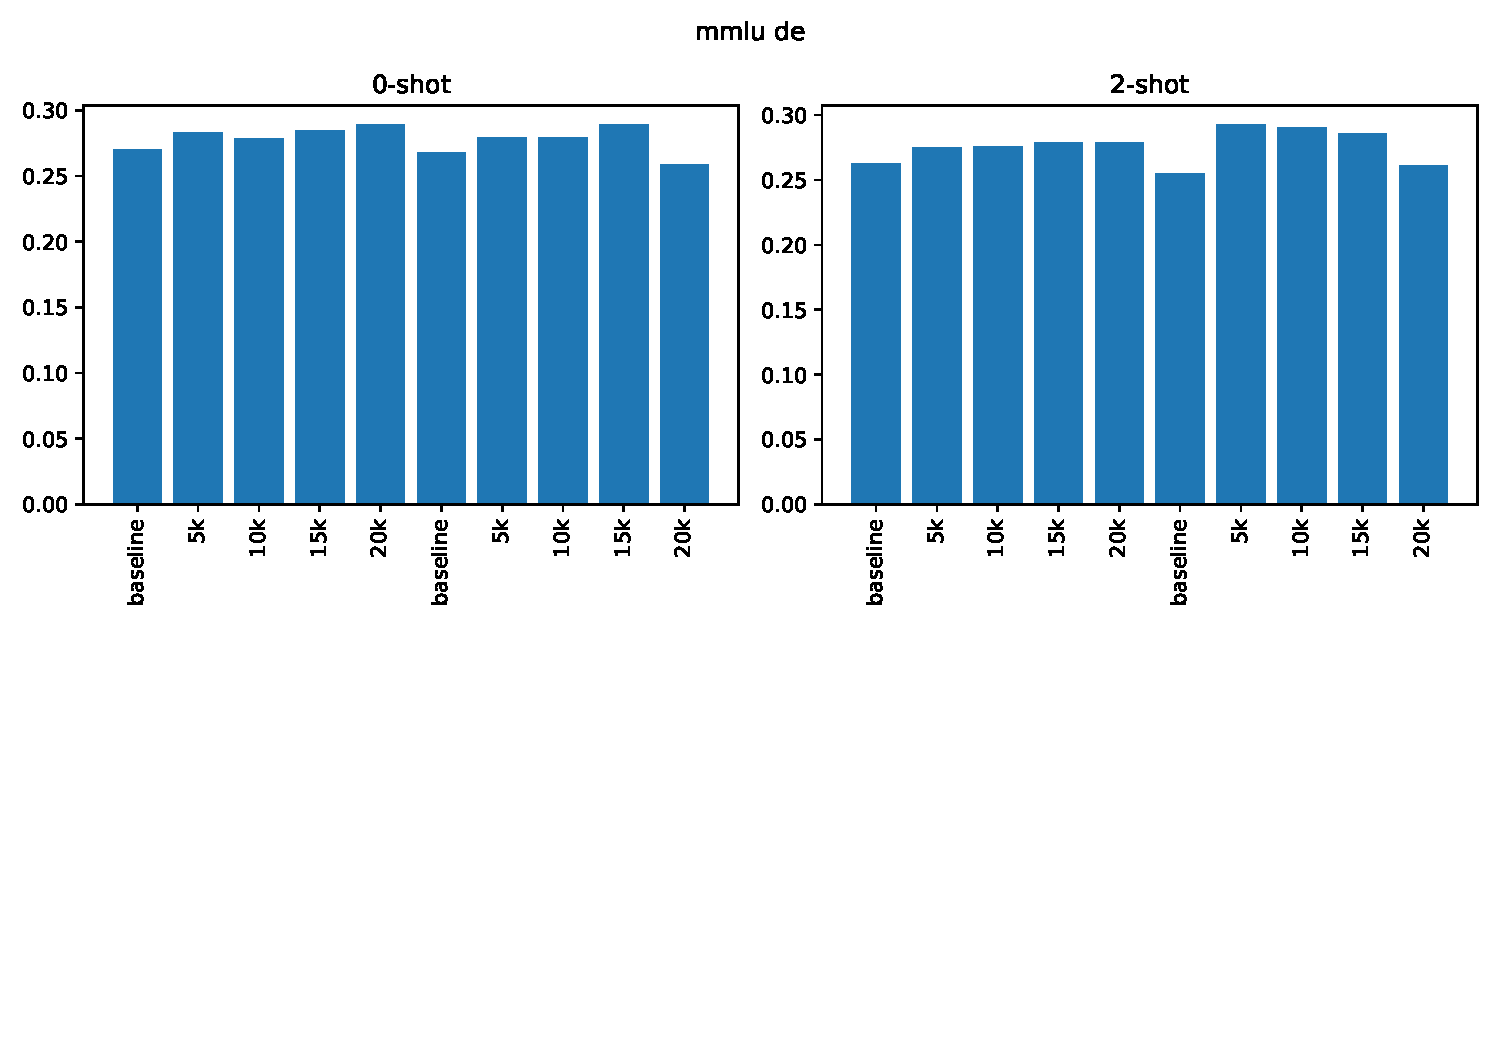
\includegraphics[width=\linewidth,clip,trim=0 5cm 0 0]{images/plot_mmlu_de.pdf}
%     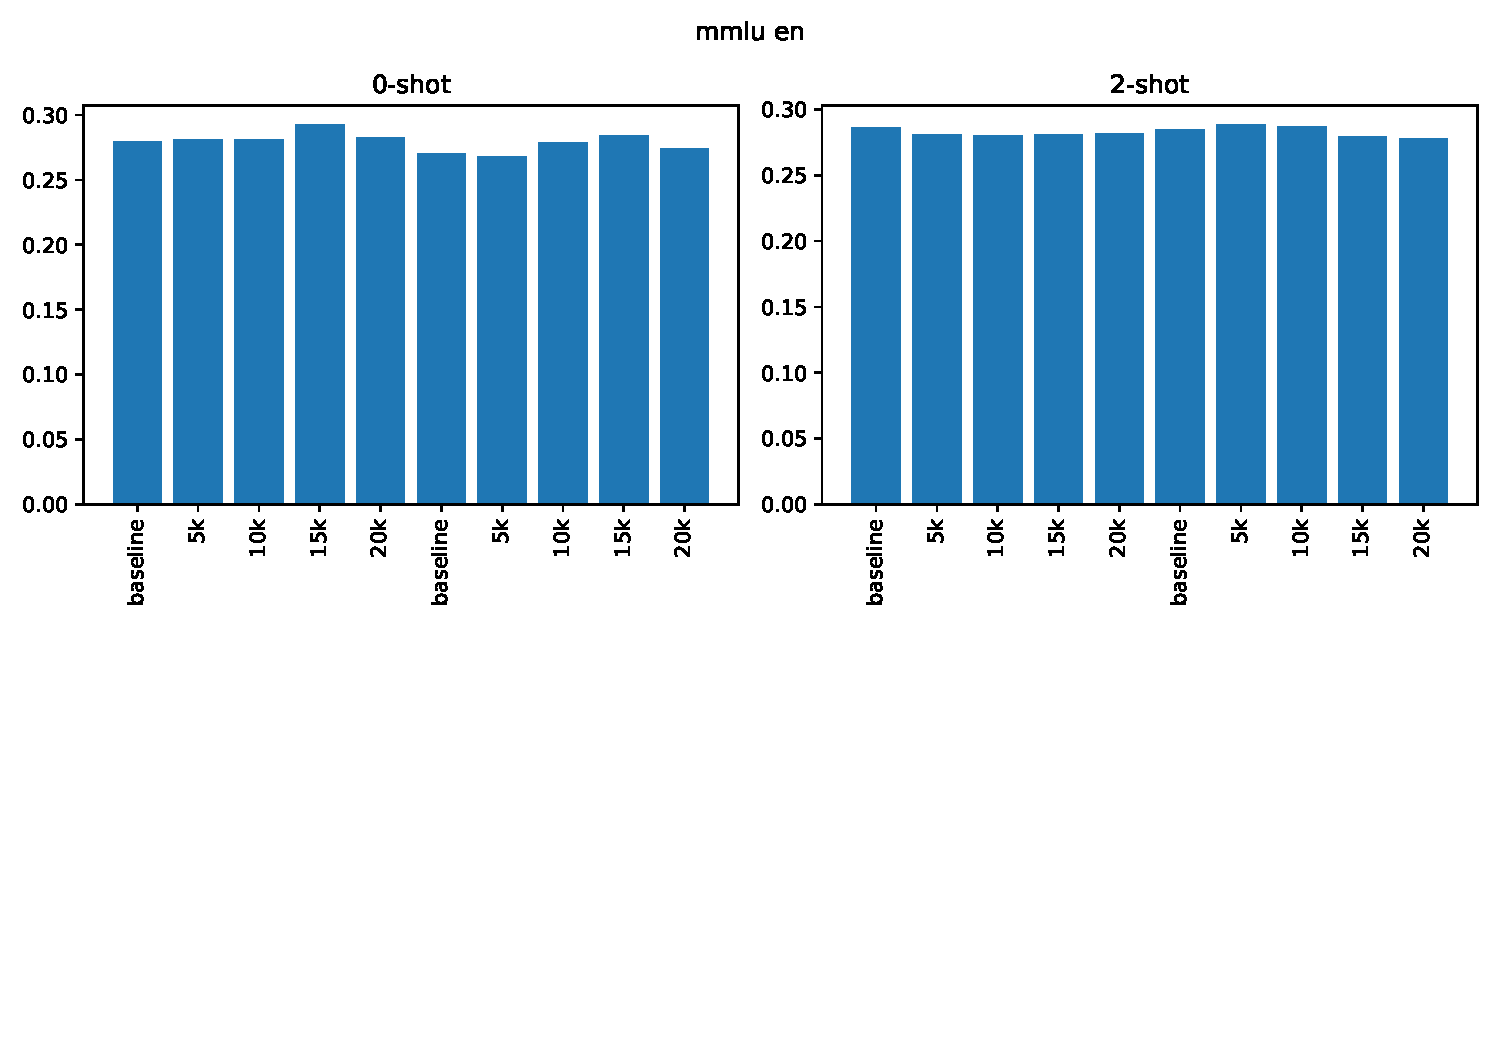
\includegraphics[width=\linewidth,clip,trim=0 5cm 0 0]{images/plot_mmlu_en.pdf}
%     \caption{Caption}
%     \label{fig:plot_all3}
% \end{figure*}

% \begin{figure*}
%     \centering
%     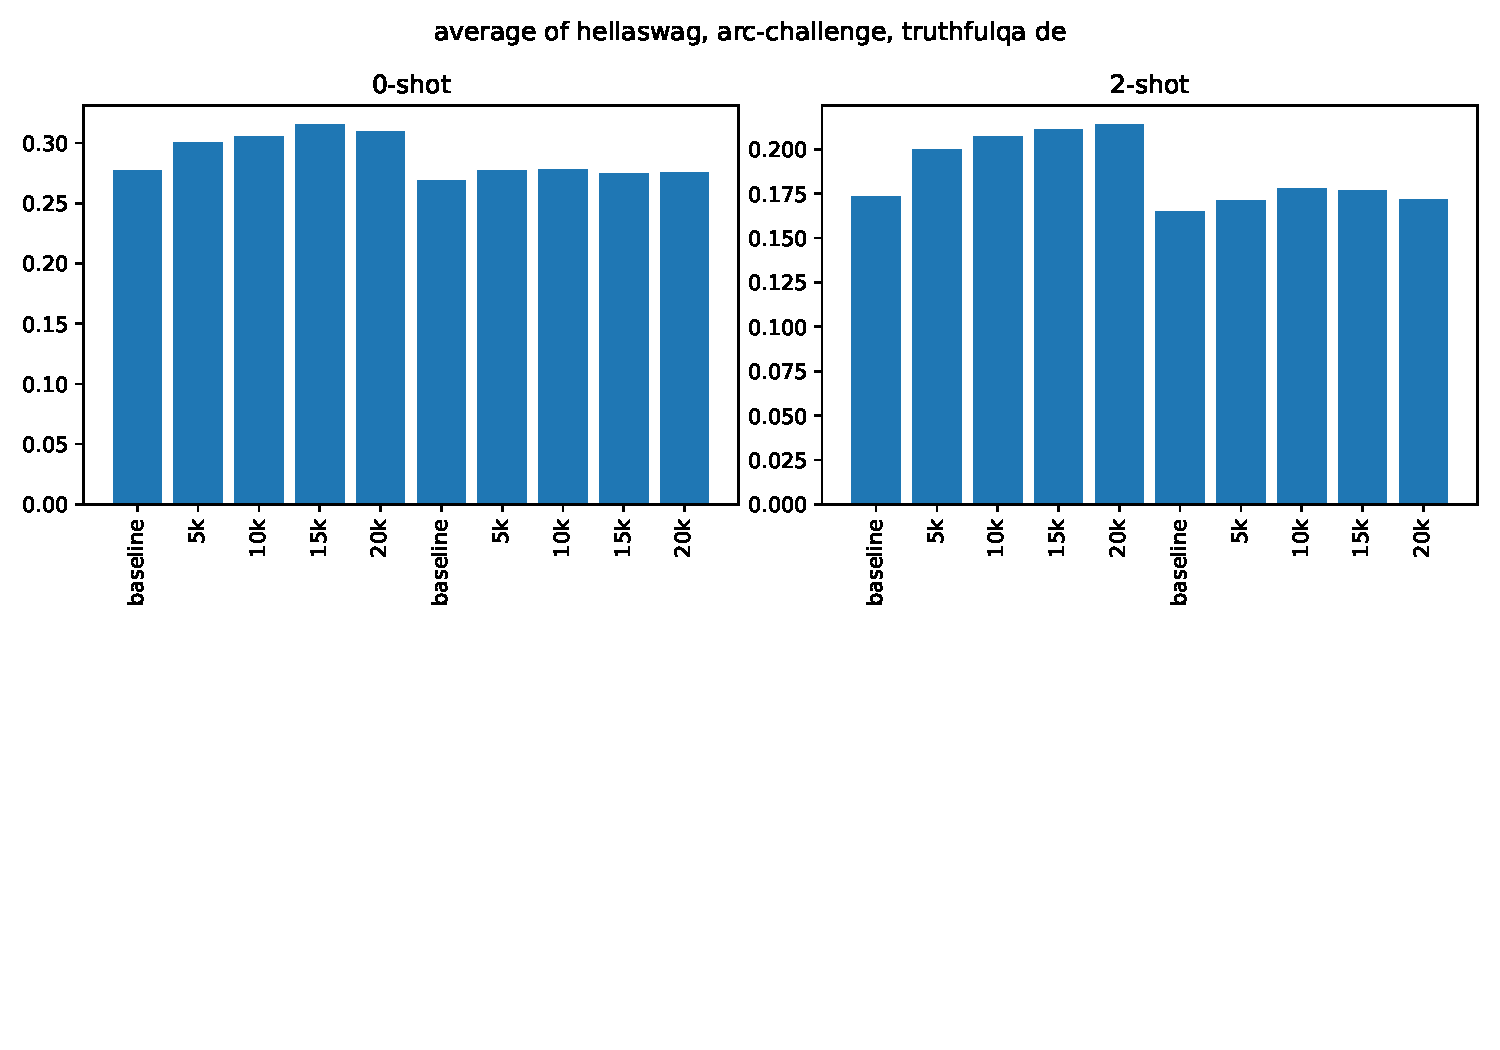
\includegraphics[width=\linewidth,clip,trim=0 5cm 0 0]{images/plot_de_avg.pdf}
%     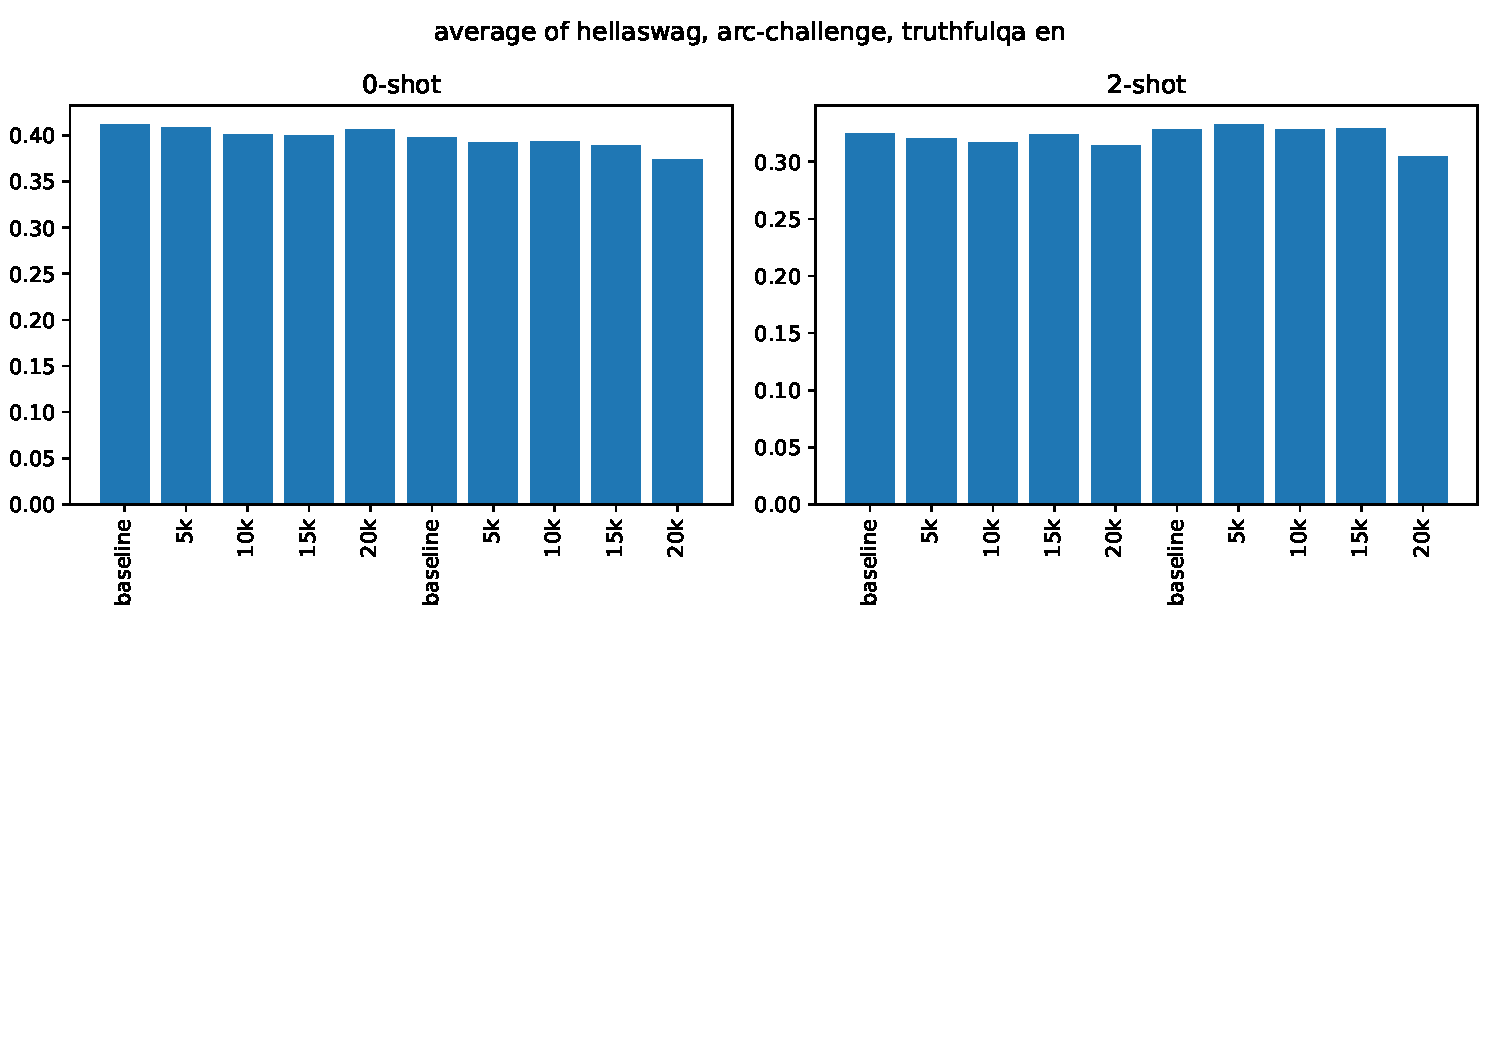
\includegraphics[width=\linewidth,clip,trim=0 5cm 0 0]{images/plot_en_avg.pdf}
%     \caption{Caption}
%     \label{fig:plot_all4}
% \end{figure*}




\end{document}